\documentclass[10pt]{article}
\usepackage[utf8]{inputenc}
\usepackage[T1]{fontenc}
\usepackage{amsmath}
\usepackage{amsfonts}
\usepackage{amssymb}
\usepackage[version=4]{mhchem}
\usepackage{stmaryrd}
\usepackage{mathrsfs}
\usepackage{graphicx}
\usepackage[export]{adjustbox}
\graphicspath{ {./images/} }
\usepackage{bbold}

\title{Nearest Neighbor Classifiers }

\author{}
\date{}


\begin{document}
\maketitle
and

the Curse of Dimensionality

Machine Learning Course - CS-433

Oct 25, 2023

Nicolas Flammarion

EPFL

\section*{Supervised machine learning}
We observe some data $S_{\text {train }}=\left\{x_{n}, y_{n}\right\}_{n=1}^{N} \in \mathscr{X} \times \mathscr{Y}$

Goal: given a new observation $x$, we want to predict its label $y$

How:

\begin{center}
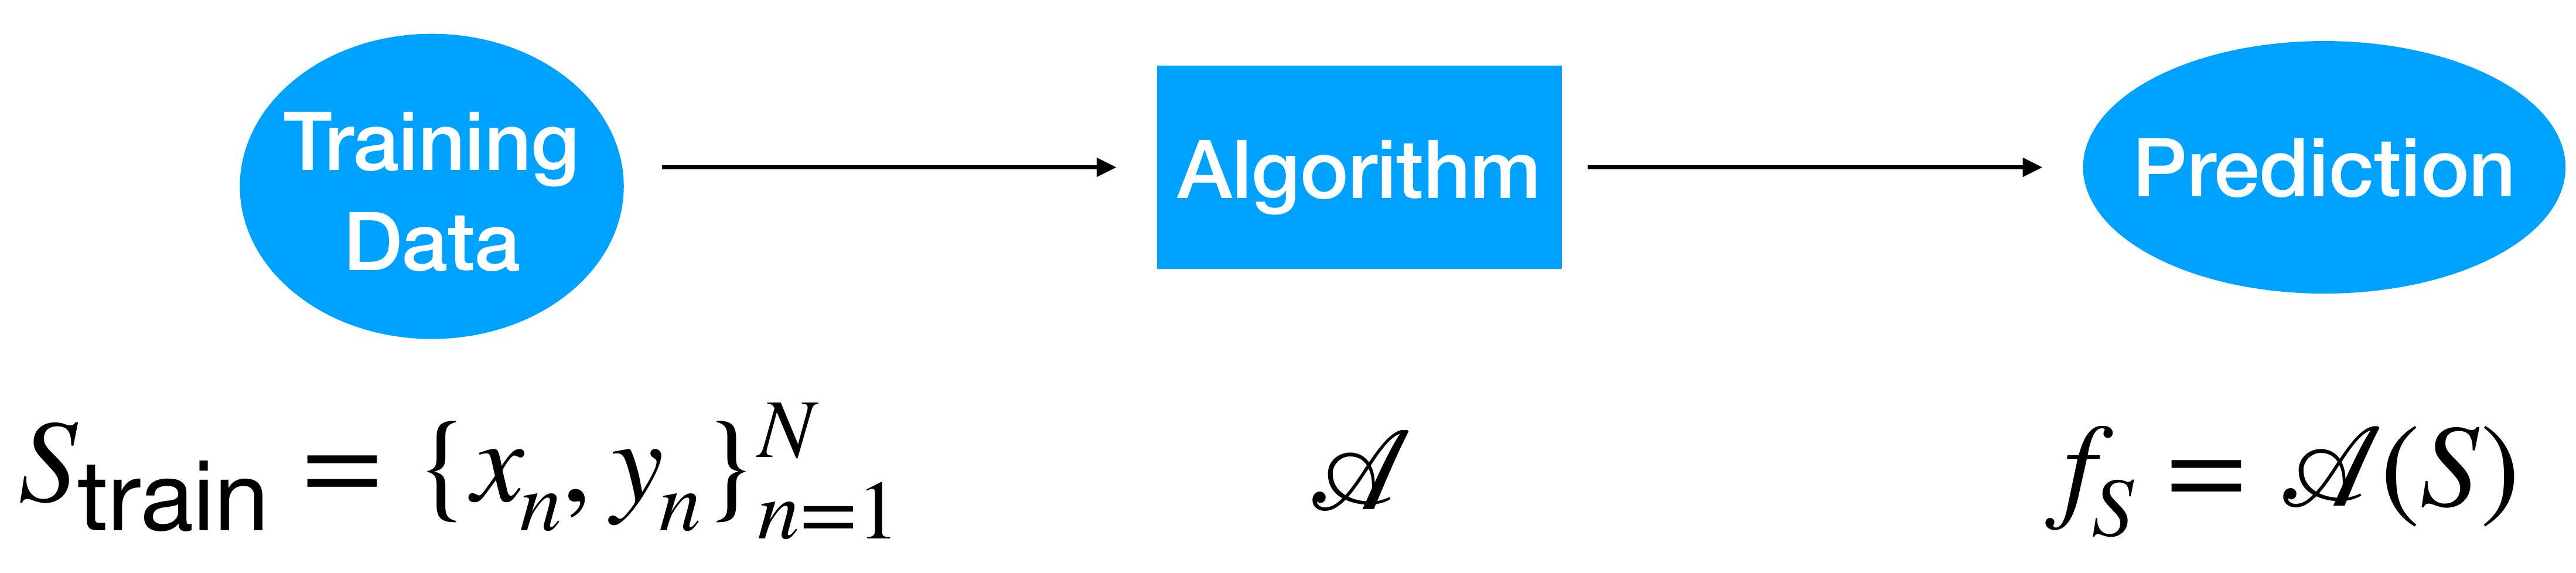
\includegraphics[max width=\textwidth]{2023_12_30_f937b0007b5d87b39f79g-02}
\end{center}

\section*{Nearest neighbor function}
$$
\begin{aligned}
\operatorname{nbh}_{S_{\text {train }}, k}: X & \rightarrow X^{k} \\
x & \mapsto\left\{\text { the } k \text { elements of } S_{\text {train }} \text { closest to } x\right\}
\end{aligned}
$$

\begin{center}
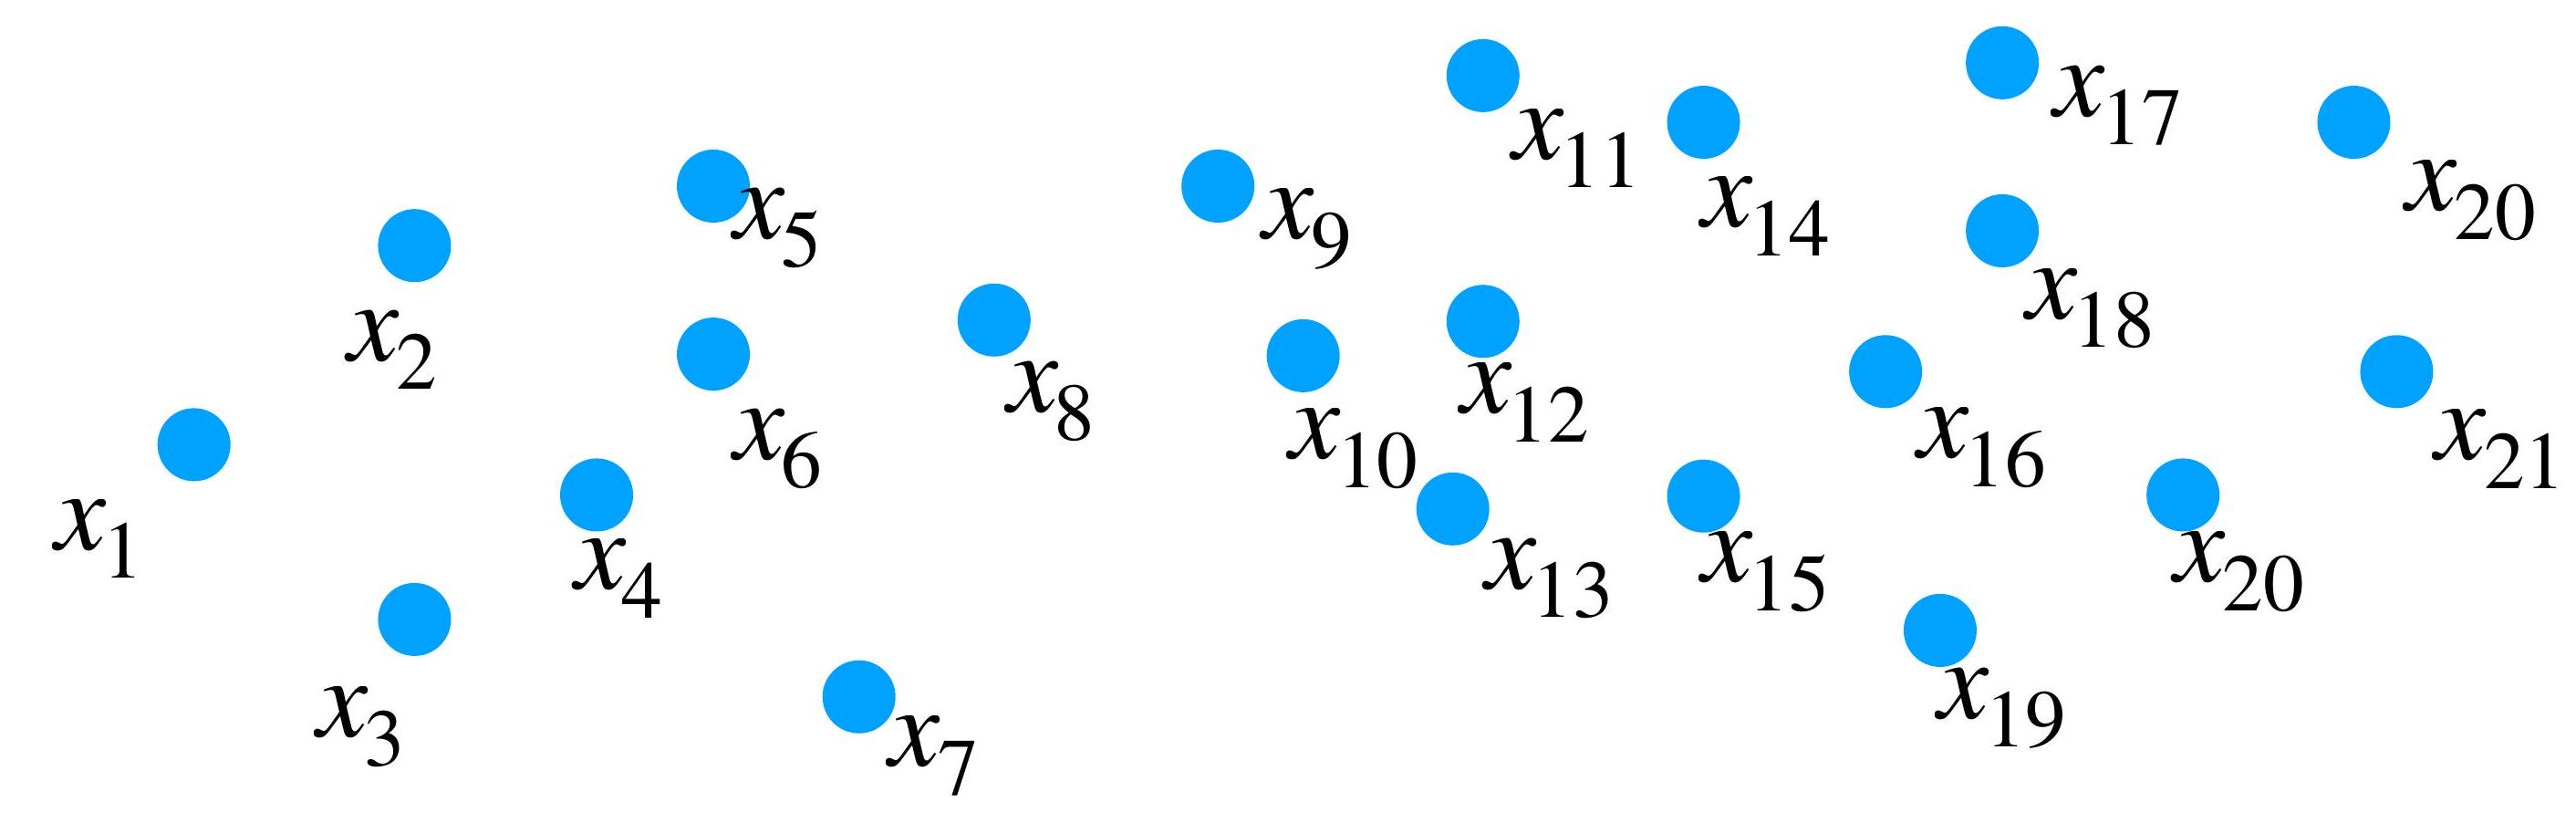
\includegraphics[max width=\textwidth]{2023_12_30_f937b0007b5d87b39f79g-03}
\end{center}

\section*{Nearest neighbor function}
$$
\begin{aligned}
\mathrm{nbh}_{S_{\text {train }}, k}: X & \rightarrow \mathscr{X}^{k} \\
x & \mapsto\left\{\text { the } k \text { elements of } S_{\text {train }} \text { closest to } x\right\}
\end{aligned}
$$

\begin{center}
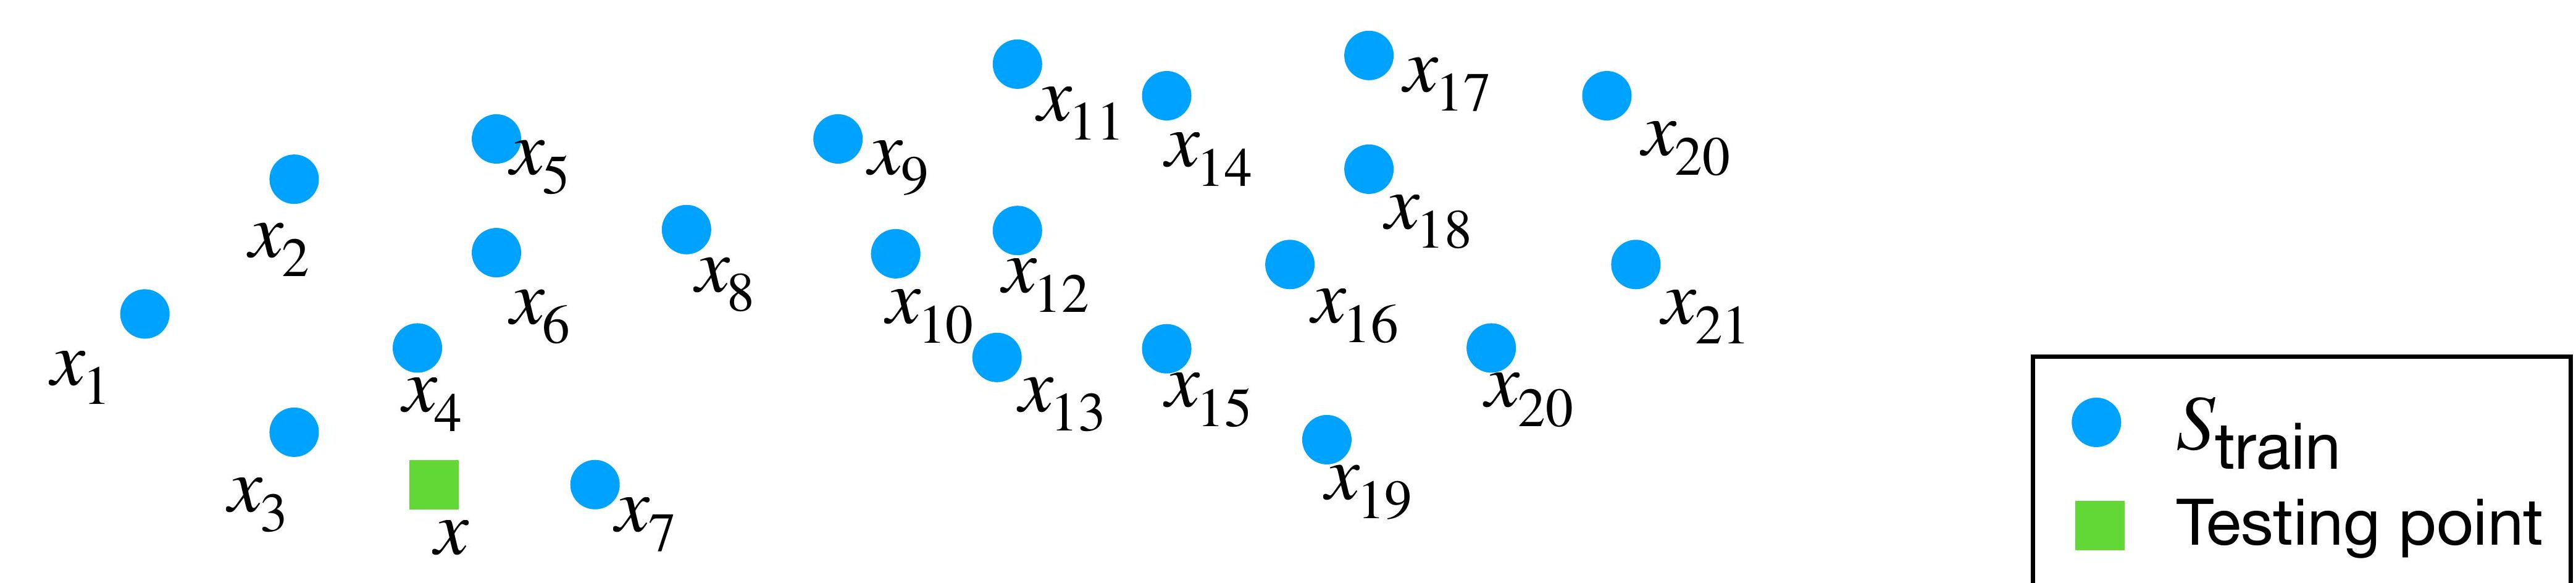
\includegraphics[max width=\textwidth]{2023_12_30_f937b0007b5d87b39f79g-04}
\end{center}

$\operatorname{nbh}_{S_{\text {train }}, 3}(x)=$ ?

\section*{Nearest neighbor function}
$$
\begin{aligned}
\mathrm{nbh}_{S_{\text {train }}, k}: X & \rightarrow \mathscr{X}^{k} \\
x & \mapsto\left\{\text { the } k \text { elements of } S_{\text {train }} \text { closest to } x\right\}
\end{aligned}
$$

\begin{center}
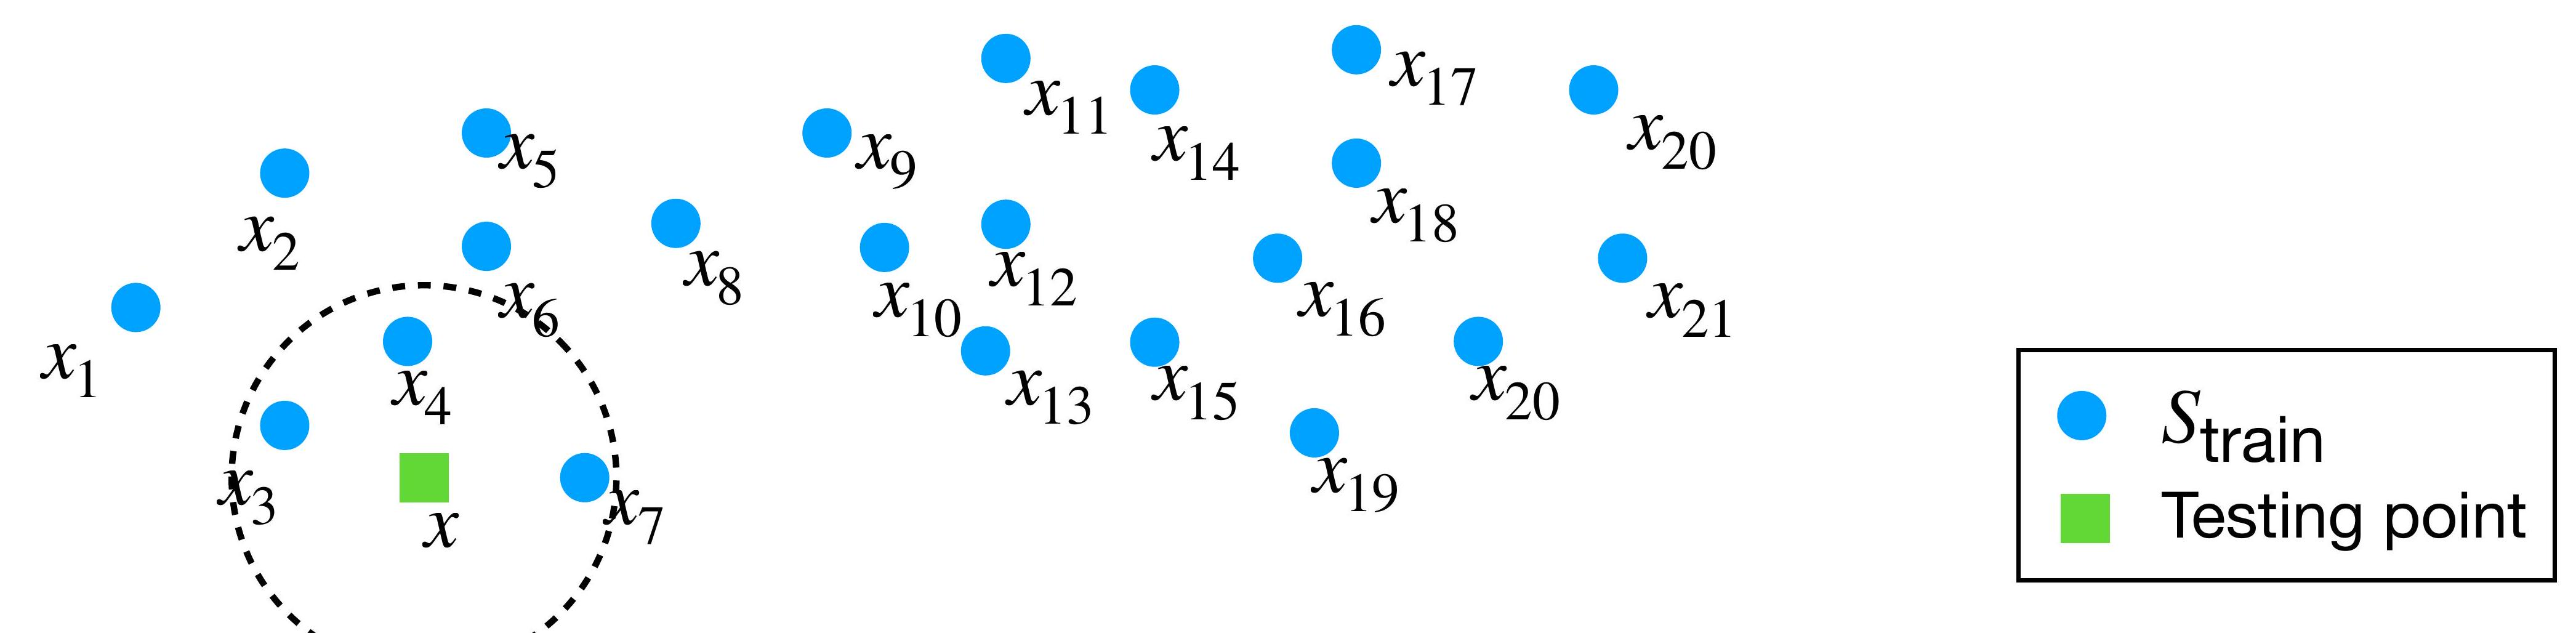
\includegraphics[max width=\textwidth]{2023_12_30_f937b0007b5d87b39f79g-05}
\end{center}

$\operatorname{nbh}_{S_{\text {train }}, 3}(x)=\left\{x_{3}, x_{4}, x_{7}\right\}$

\section*{Nearest neighbor function}
$$
\begin{aligned}
\mathrm{nbh}_{S_{\text {train }}, k}: X & \rightarrow \mathscr{X}^{k} \\
x & \mapsto\left\{\text { the } k \text { elements of } S_{\text {train }} \text { closest to } x\right\}
\end{aligned}
$$

\begin{center}
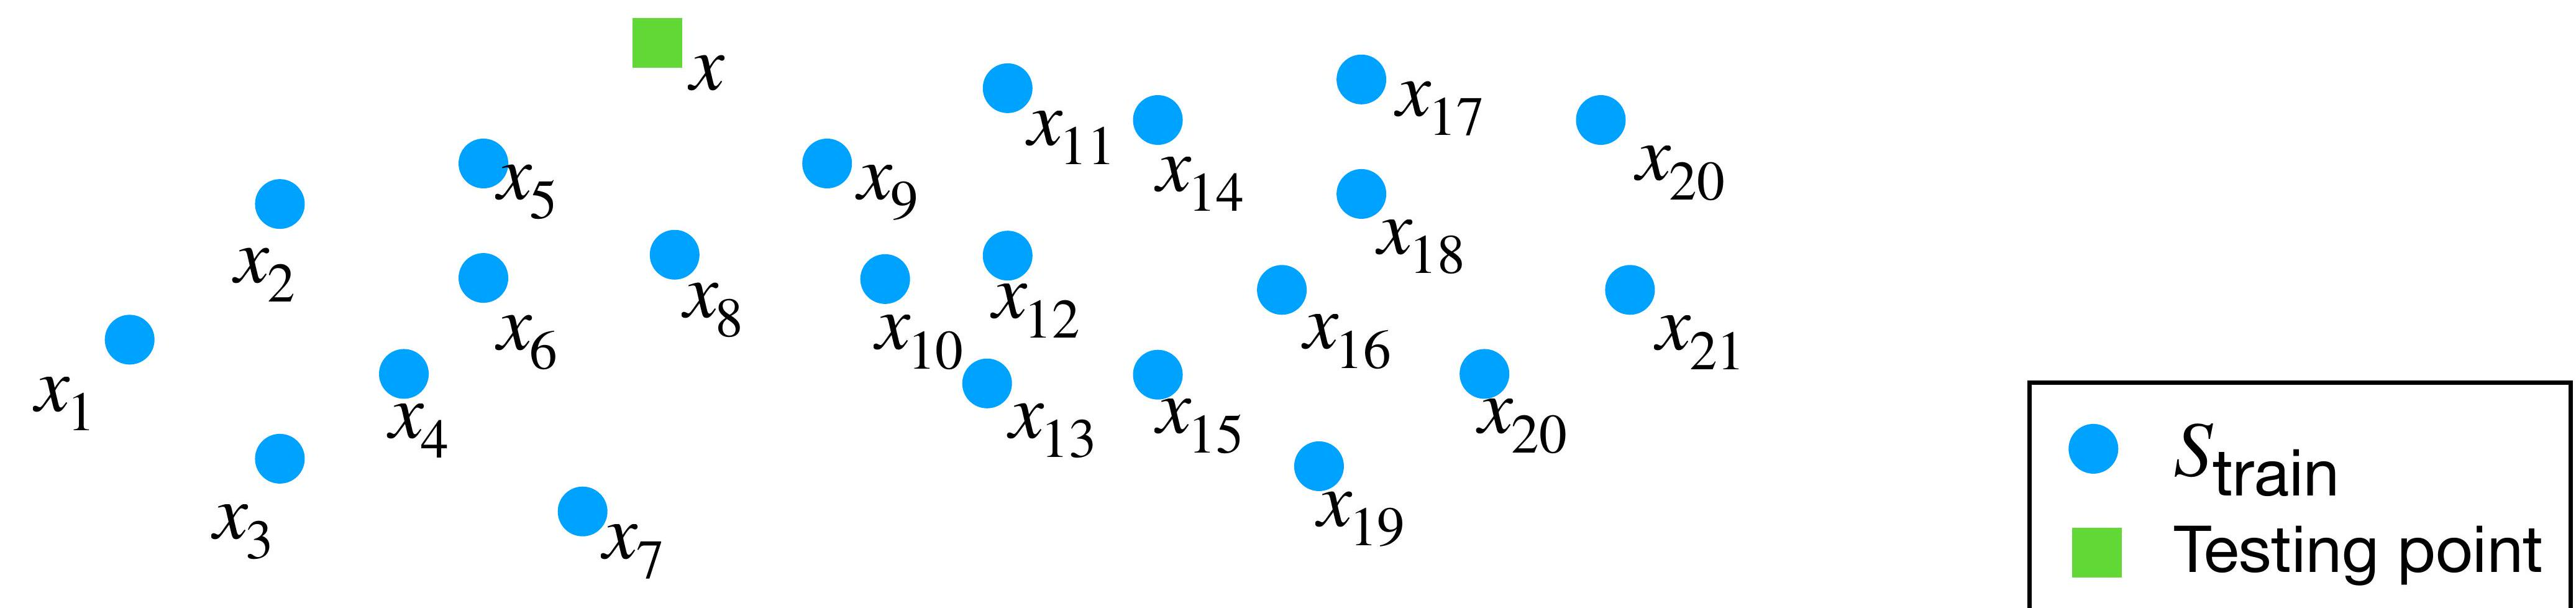
\includegraphics[max width=\textwidth]{2023_12_30_f937b0007b5d87b39f79g-06}
\end{center}

$\operatorname{nbh}_{S_{\text {train }}, 2}(x)=?$

\section*{Nearest neighbor function}
$$
\begin{aligned}
\mathrm{nbh}_{S_{\text {train }}, k}: X & \rightarrow \mathscr{X}^{k} \\
x & \mapsto\left\{\text { the } k \text { elements of } S_{\text {train }} \text { closest to } x\right\}
\end{aligned}
$$

\begin{center}
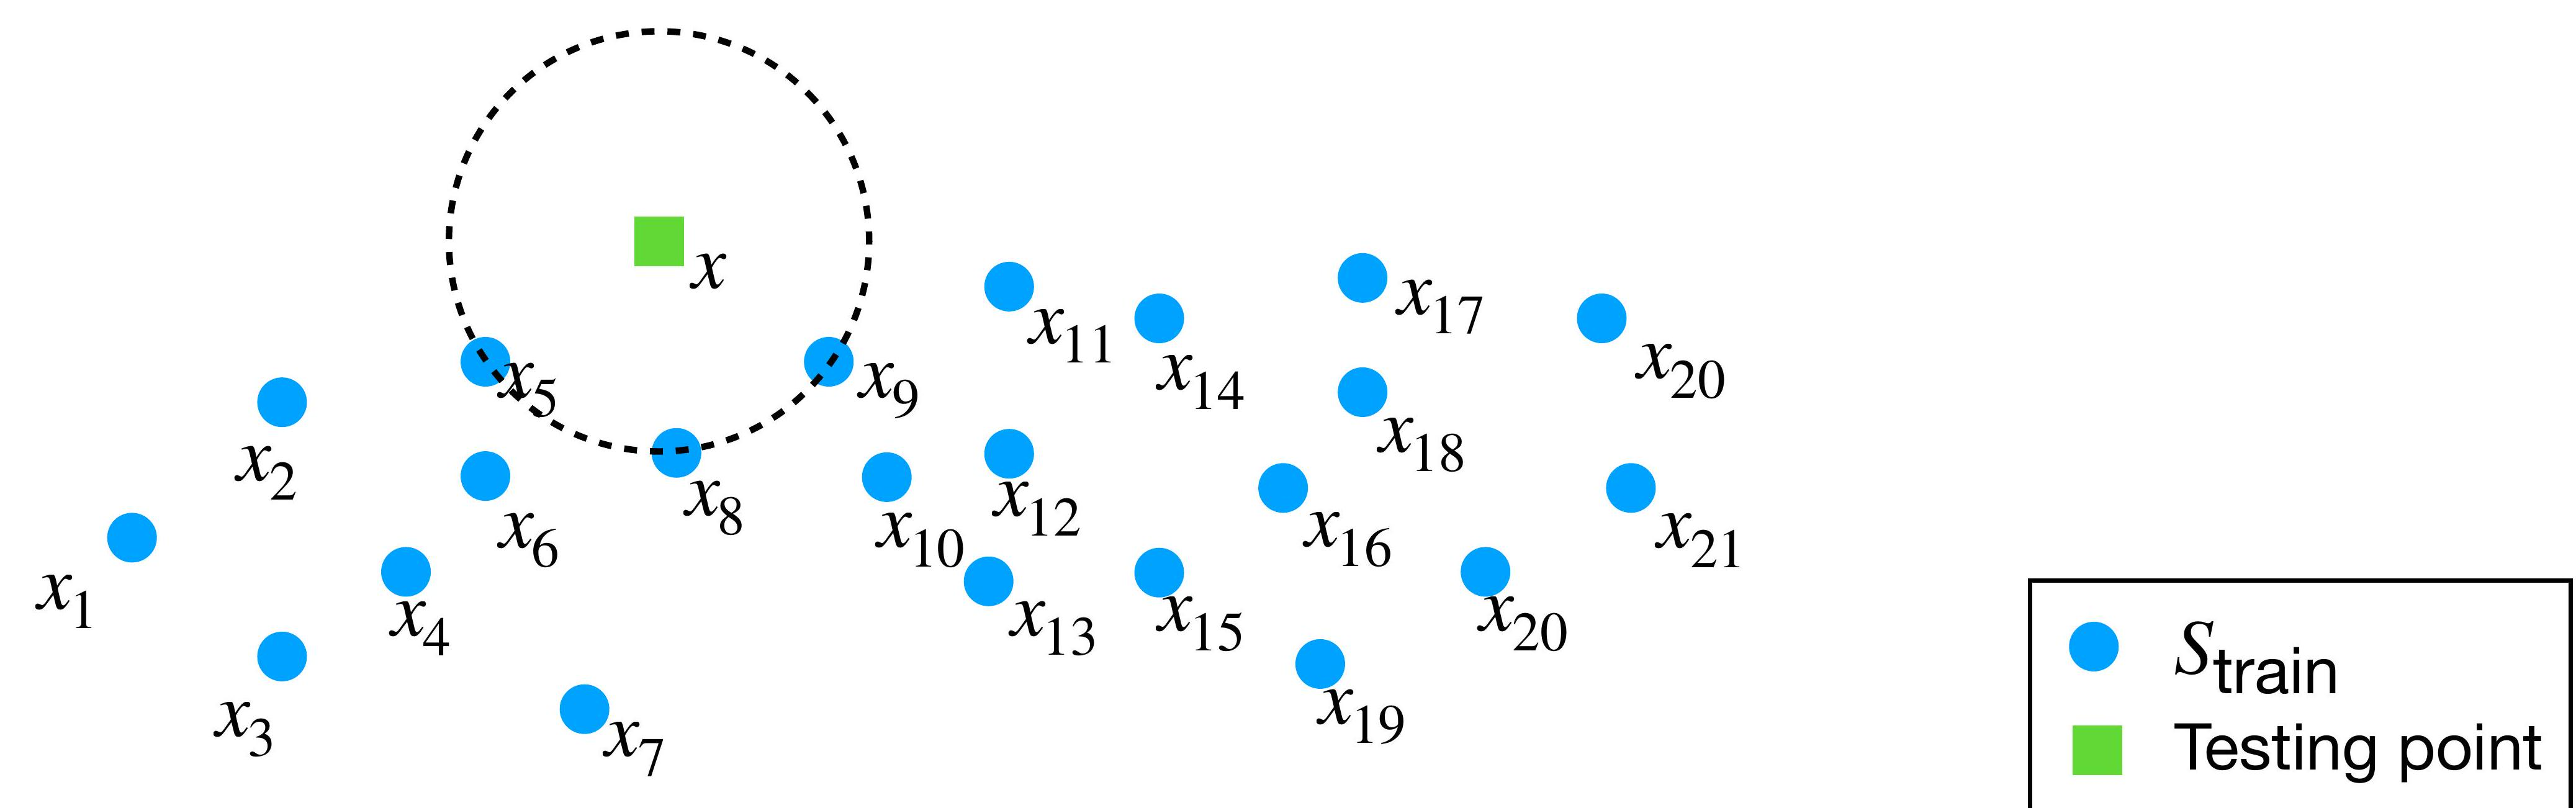
\includegraphics[max width=\textwidth]{2023_12_30_f937b0007b5d87b39f79g-07}
\end{center}

$\operatorname{nbh}_{S_{\text {train }}, 2}(x)=?$

\section*{Nearest neighbor function}
$$
\mathrm{nbh}_{S_{\text {train }, k}}: \mathscr{X} \rightarrow \mathscr{X}^{k}
$$

$x \mapsto\left\{\right.$ the $k$ elements of $S_{\text {train }}$ closest to $\left.x\right\}$

\begin{center}
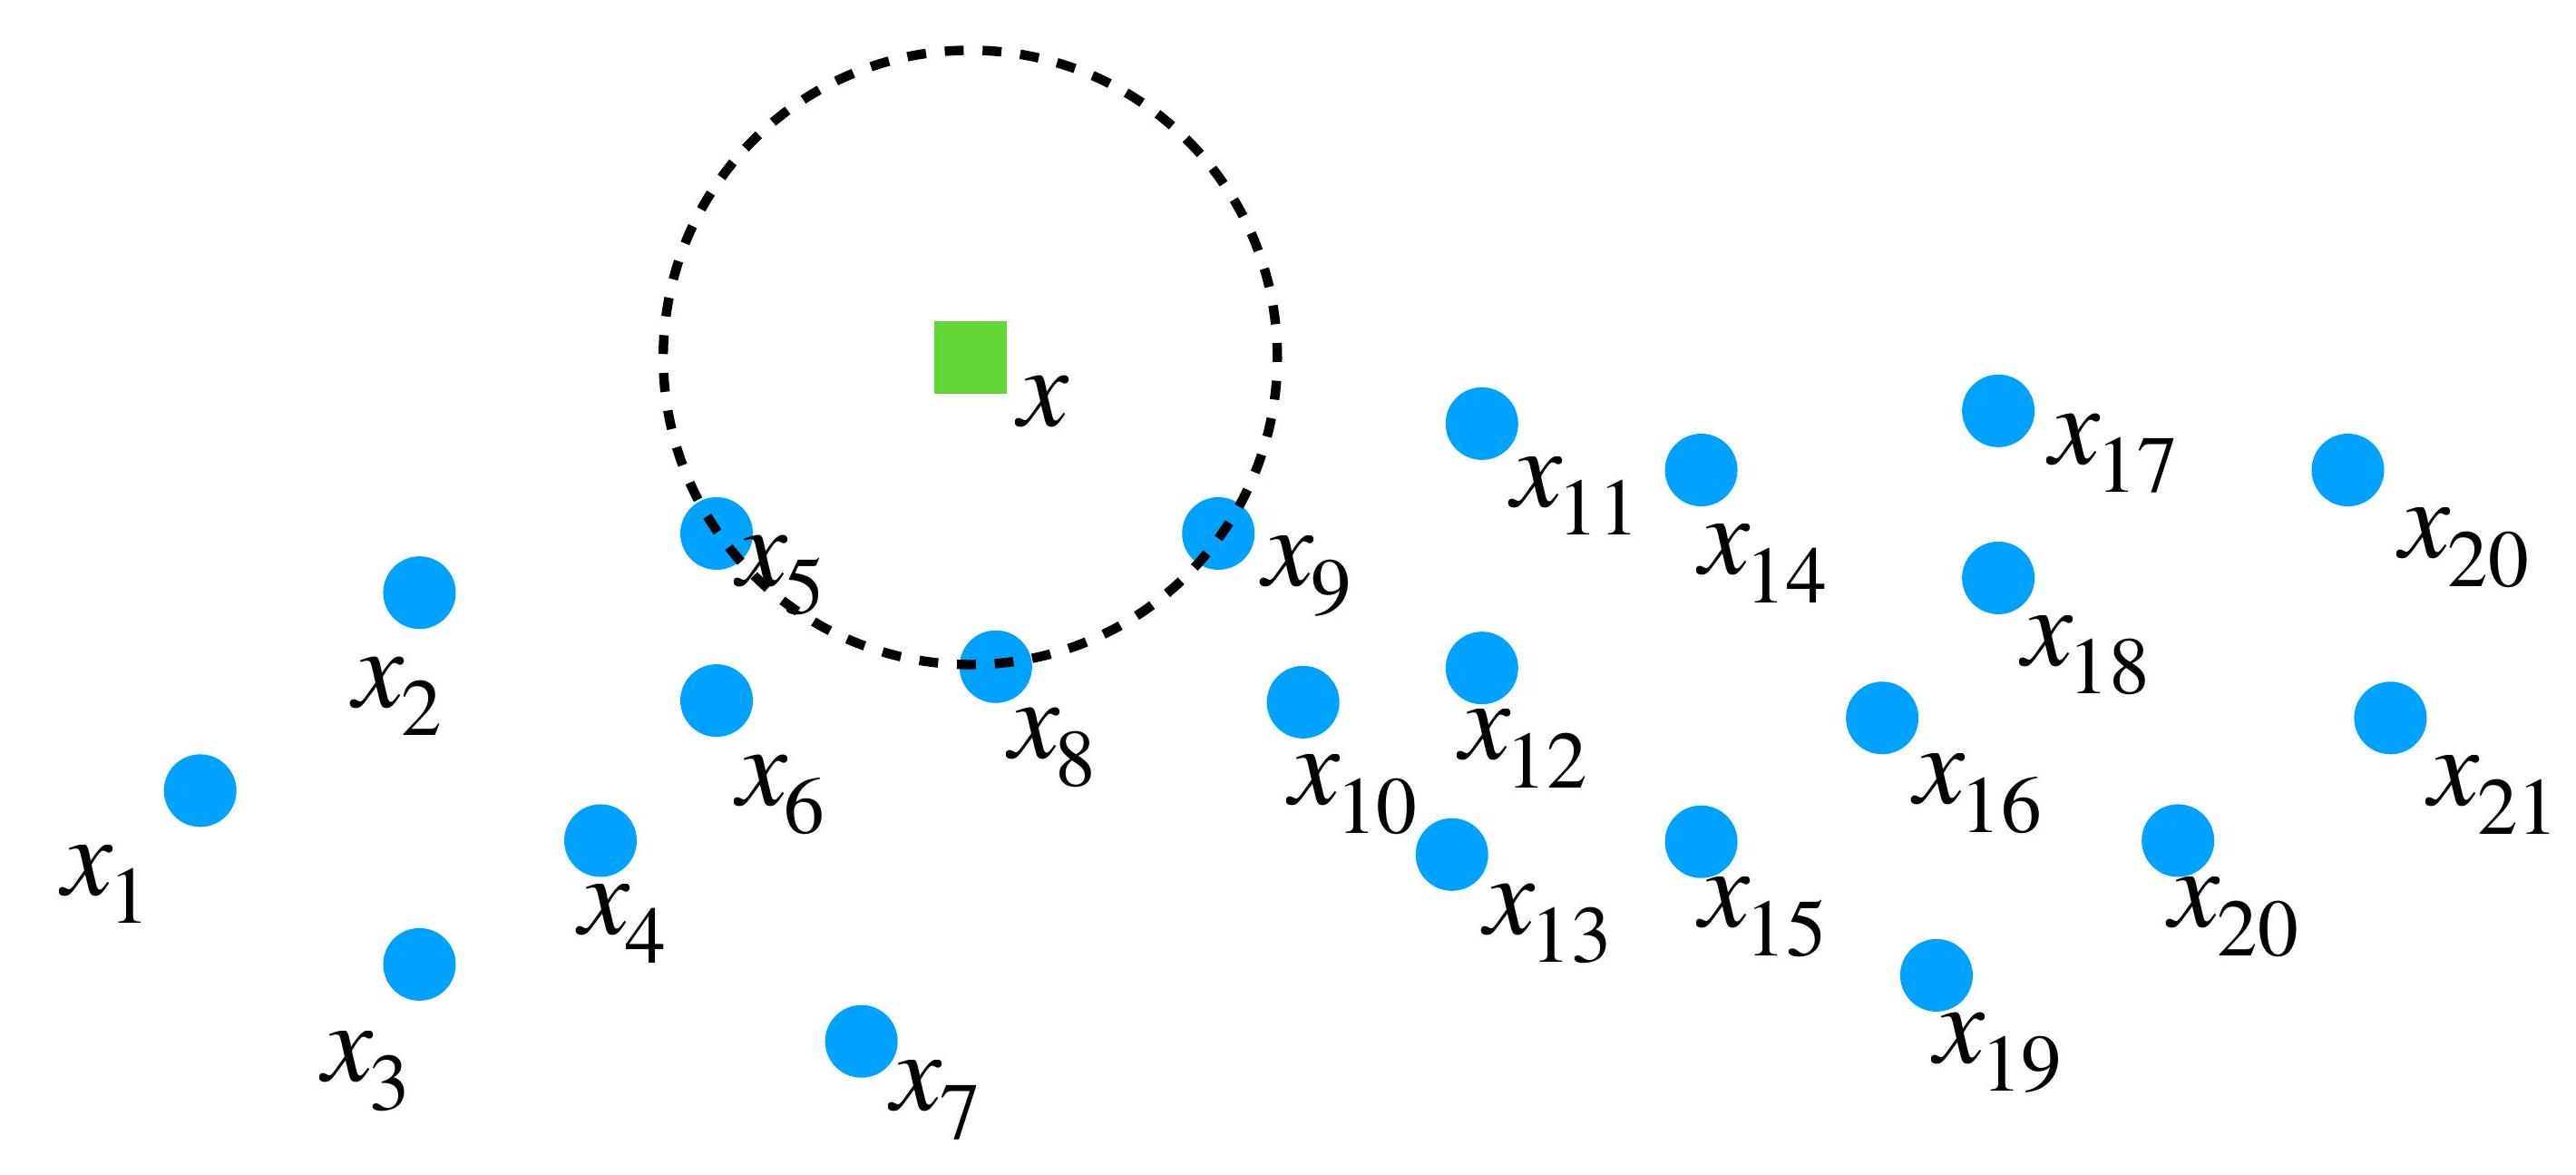
\includegraphics[max width=\textwidth]{2023_12_30_f937b0007b5d87b39f79g-08}
\end{center}

$$
\mathrm{nbh}_{S_{\text {train }}, 2}(x)=\left\{x_{5}, x_{8}\right\}
$$

\section*{Nearest neighbor function}
$$
\begin{aligned}
\mathrm{nbh}_{S_{\text {train }}, k}: X & \rightarrow \mathscr{X}^{k} \\
x & \mapsto\left\{\text { the } k \text { elements of } S_{\text {train }} \text { closest to } x\right\}
\end{aligned}
$$

\begin{center}
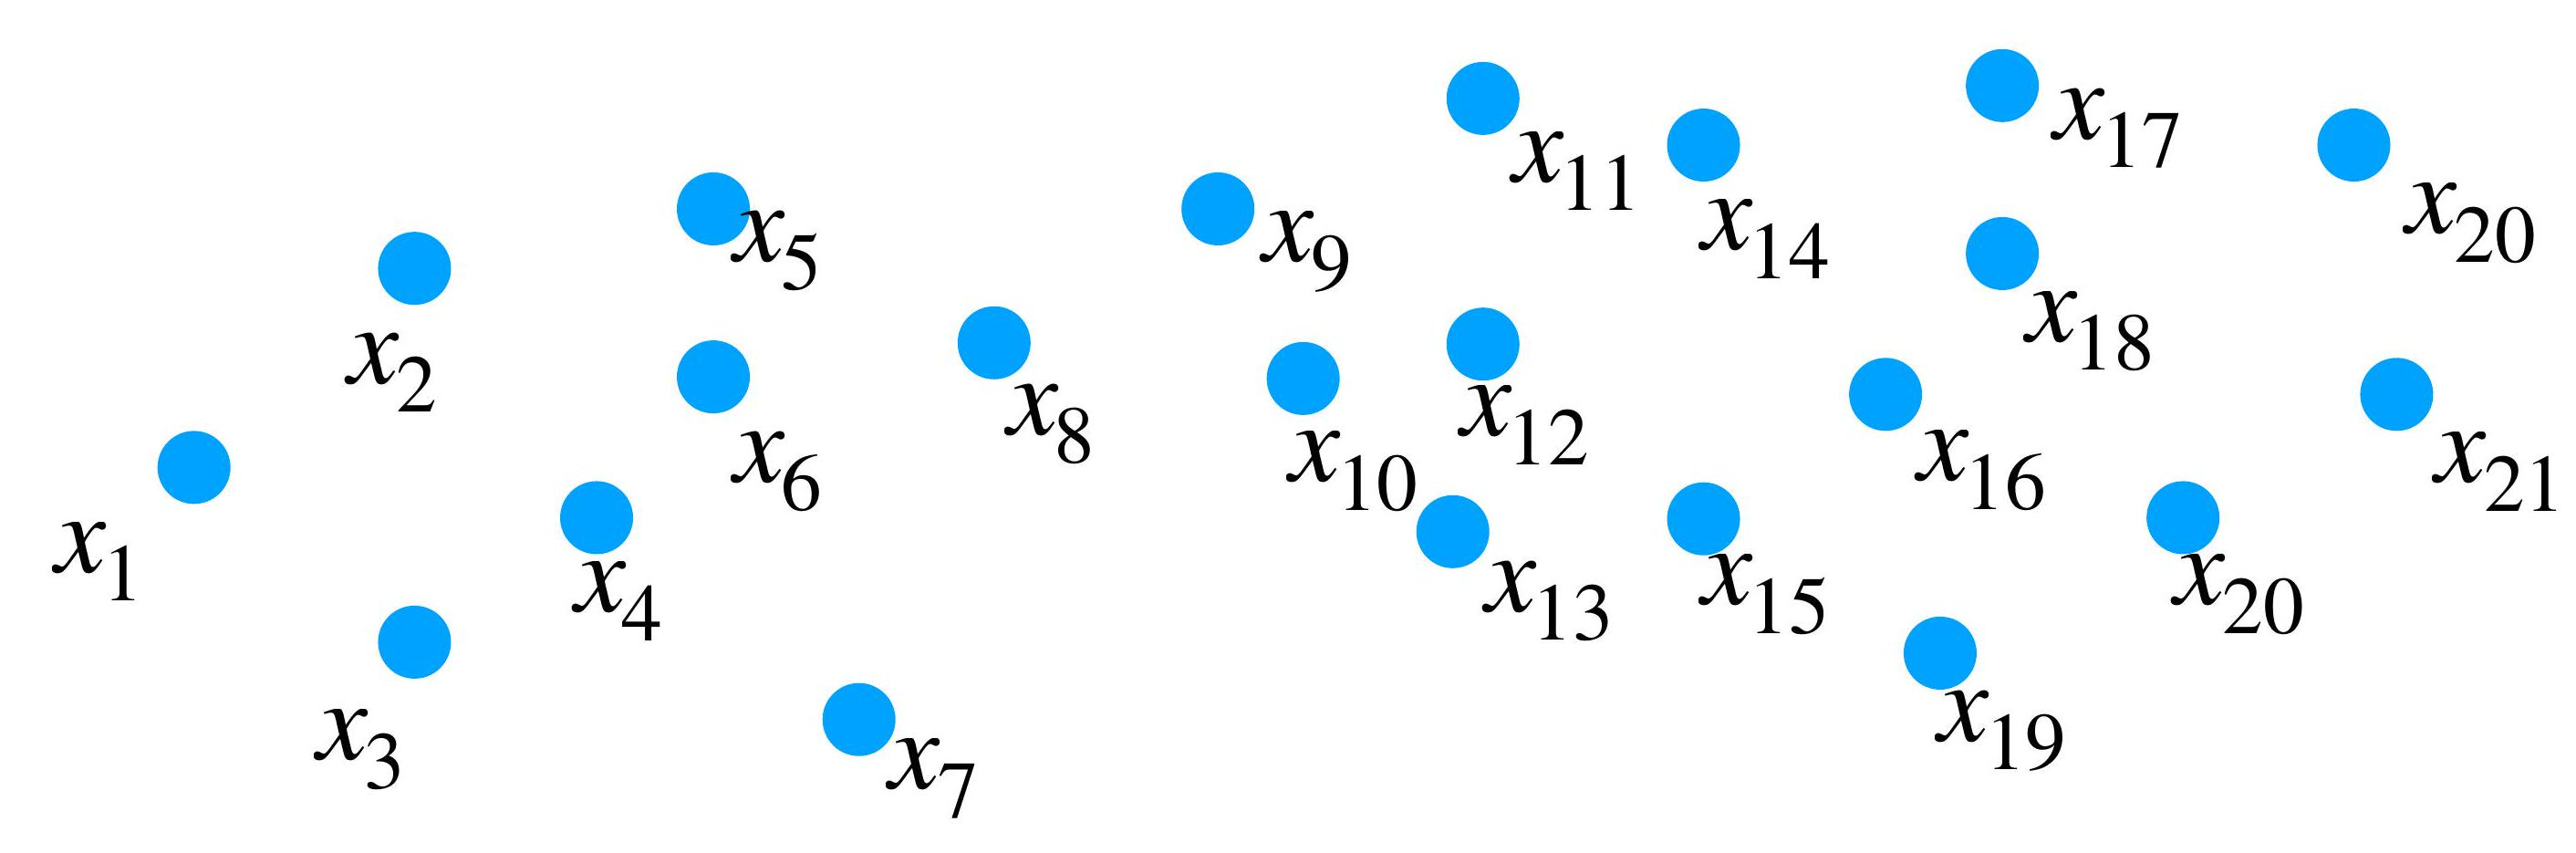
\includegraphics[max width=\textwidth]{2023_12_30_f937b0007b5d87b39f79g-09}
\end{center}

Remarks:

\begin{itemize}
  \item Different metrics can be employed
  \item High computational complexity for large $N$ (but efficient data structure may exist)
\end{itemize}

\section*{k-NN can be used for regression $(y \in \mathbb{R})$}
$$
f_{S_{\text {train }}, k}(x)=\frac{1}{k} \sum_{n: x_{n} \in n b h_{S_{\text {train }, k}}(x)} y_{n}
$$

\begin{center}
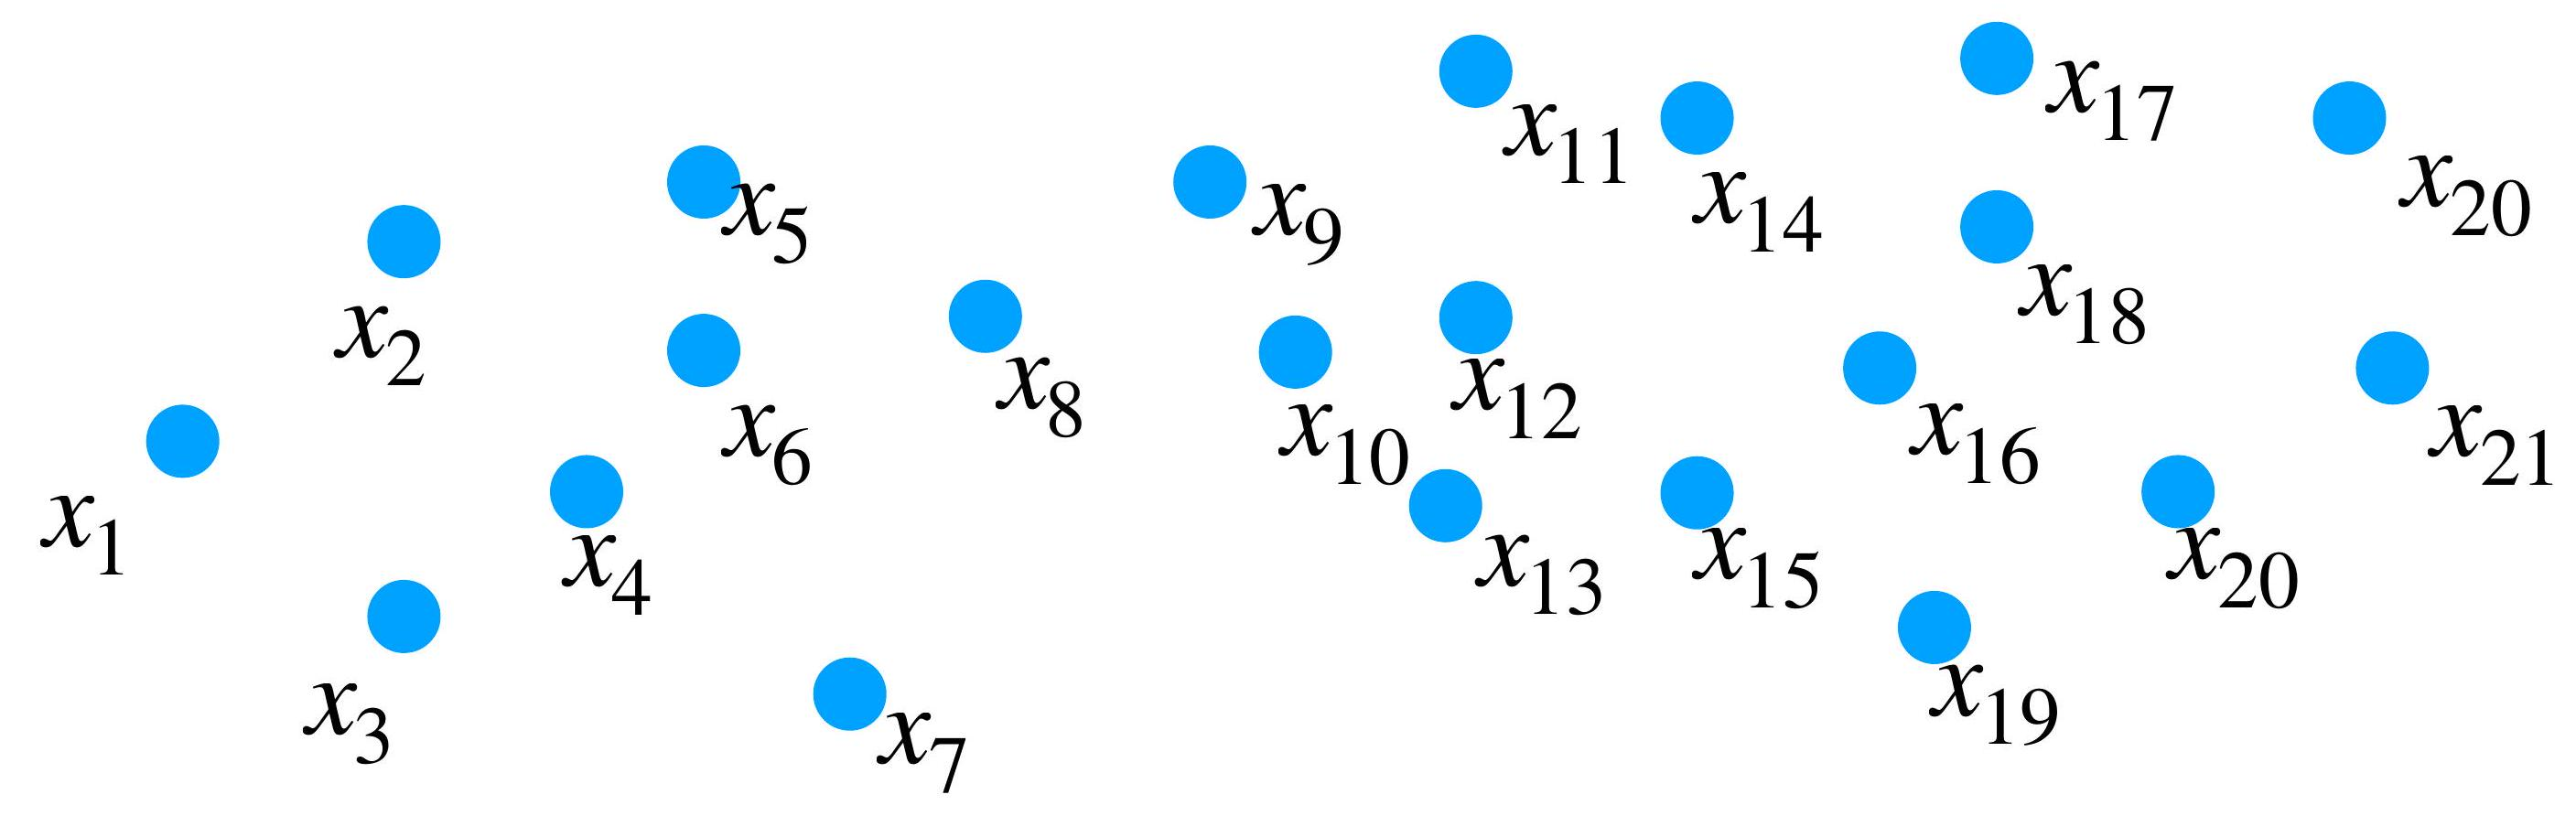
\includegraphics[max width=\textwidth]{2023_12_30_f937b0007b5d87b39f79g-10}
\end{center}

\section*{k-NN can be used for regression $(y \in \mathbb{R})$}
$$
f_{S_{\text {train }}, k}(x)=\frac{1}{k} \sum_{n: x_{n} \in n b h_{S_{\text {train }, k}(x)}} y_{n}
$$

\begin{center}
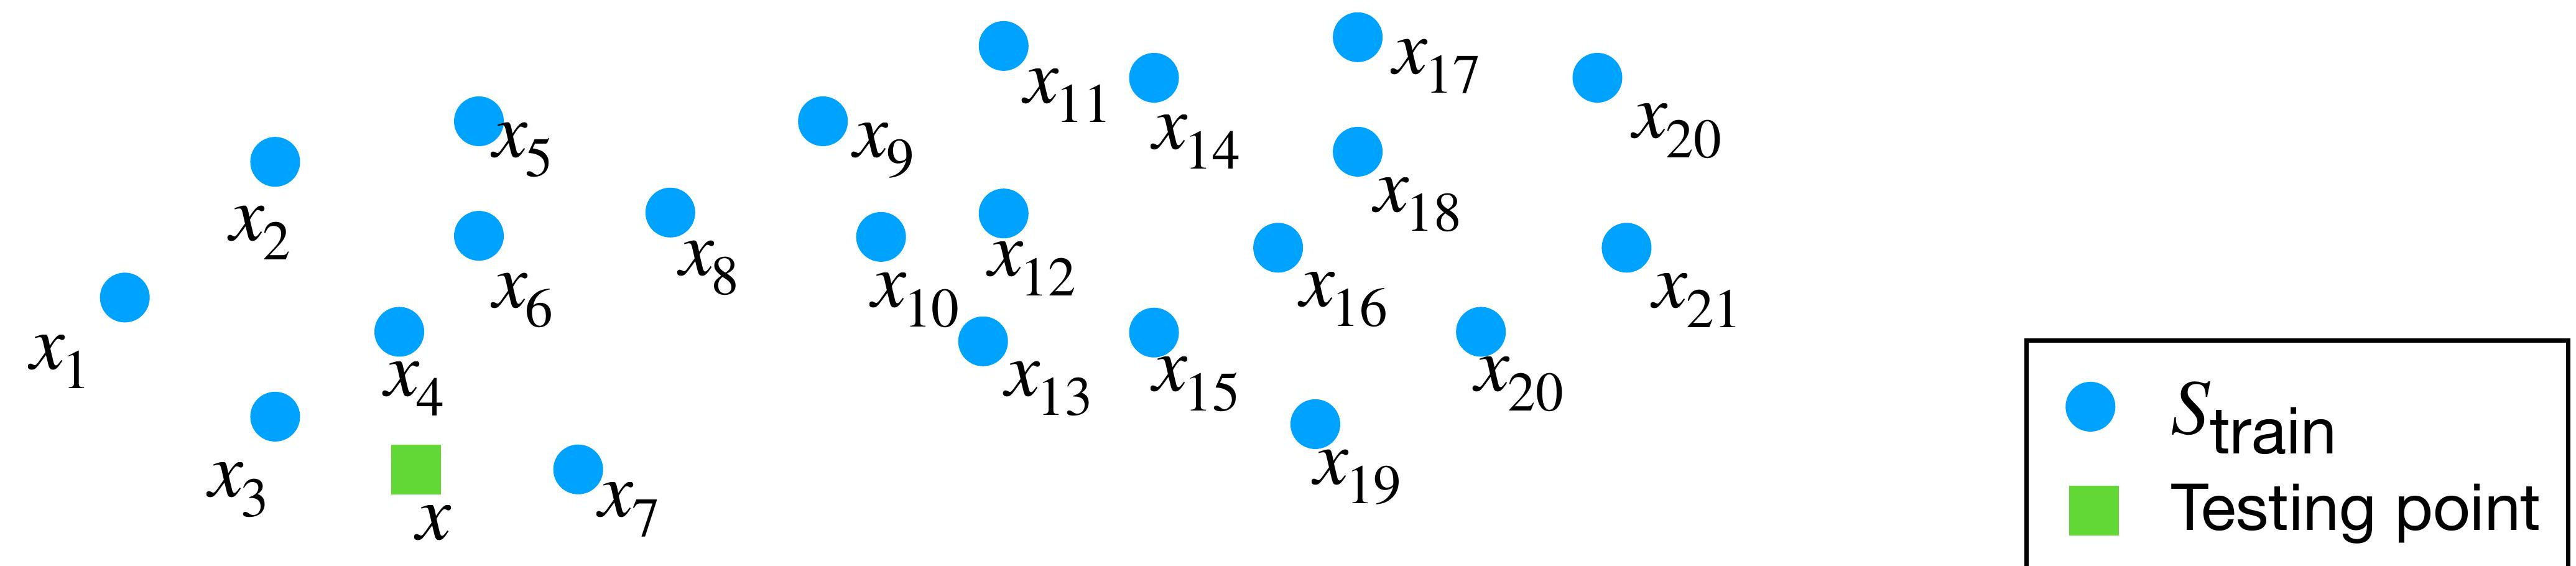
\includegraphics[max width=\textwidth]{2023_12_30_f937b0007b5d87b39f79g-11}
\end{center}

$$
f_{S_{\text {train }}, 3}(x)=?
$$

\section*{k-NN can be used for regression $(y \in \mathbb{R})$}
$$
f_{S_{\text {train }}, k}(x)=\frac{1}{k} \sum_{n: x_{n} \in n b h_{S_{\text {train }, k}(x)}} y_{n}
$$

\begin{center}
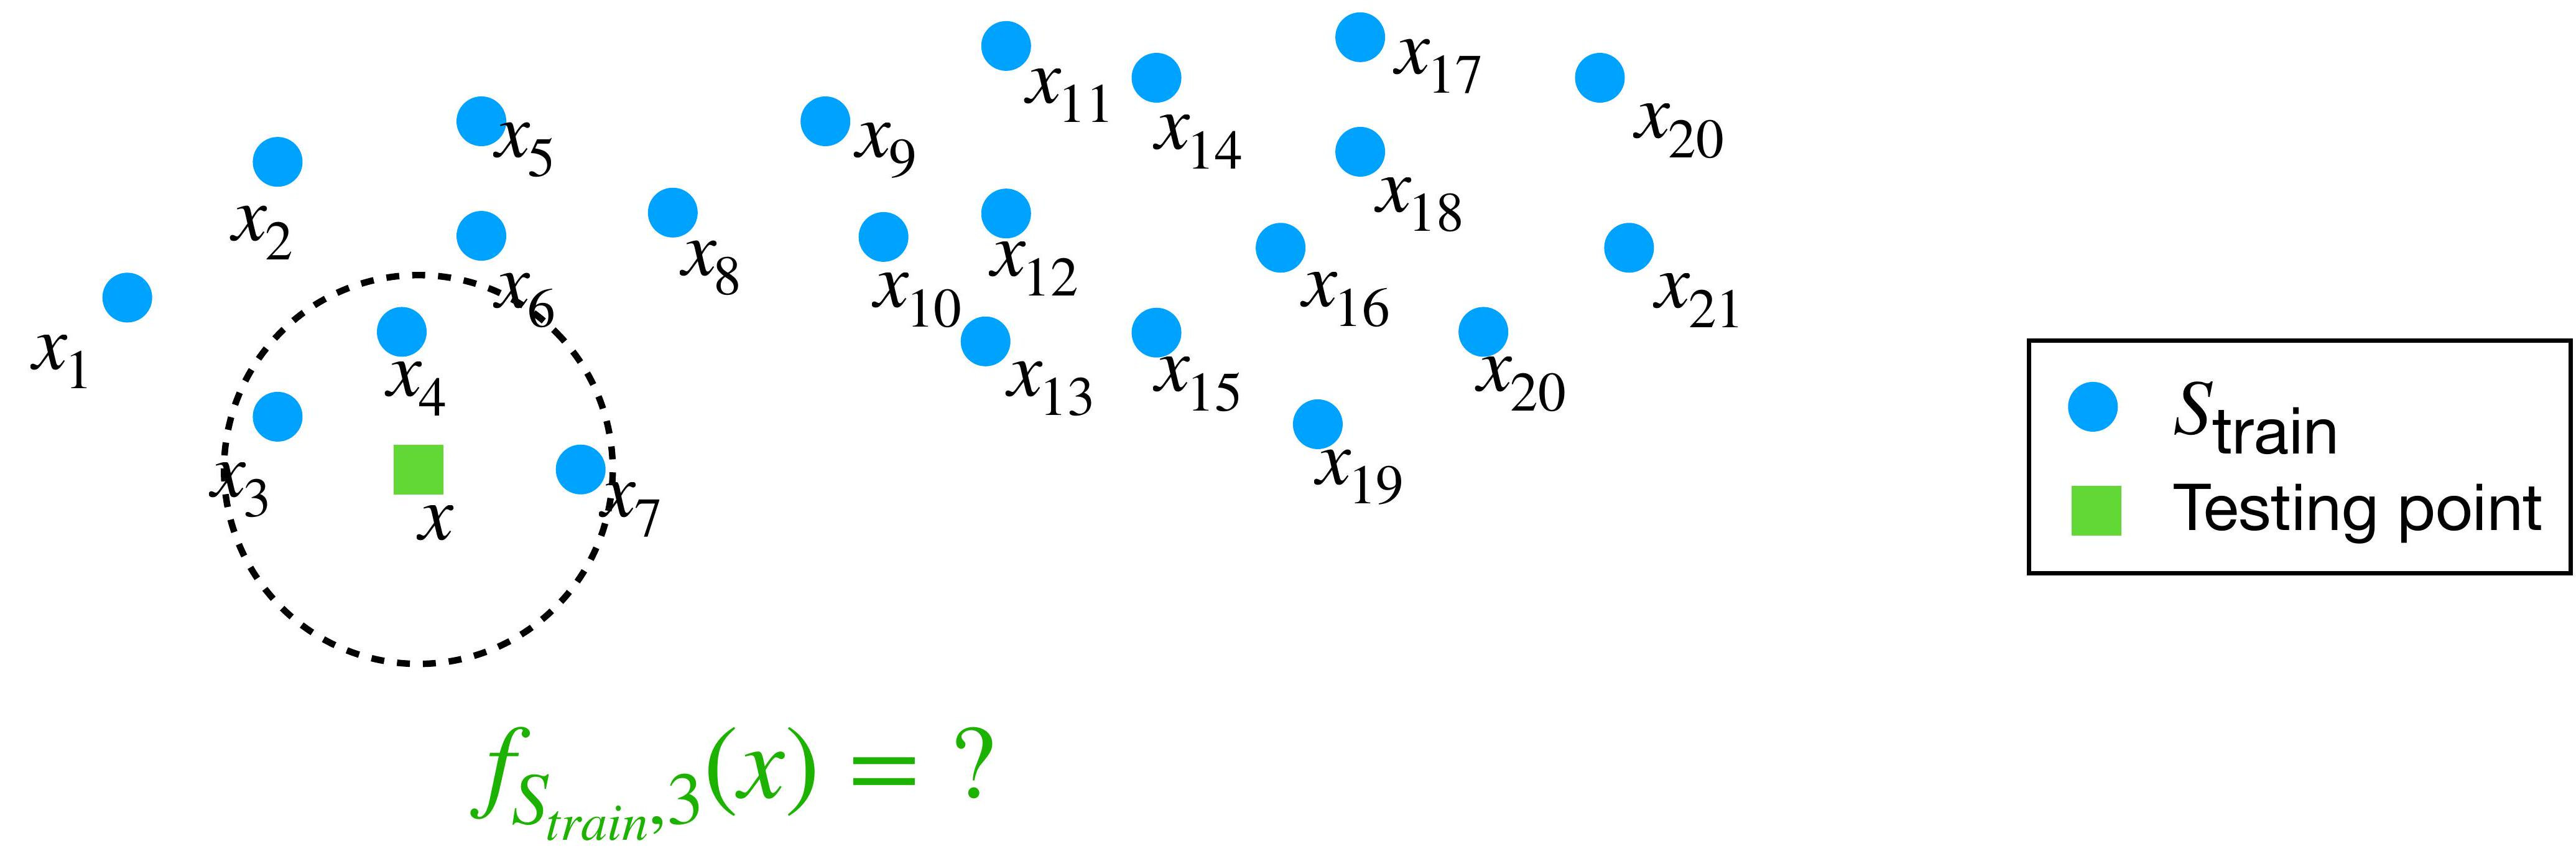
\includegraphics[max width=\textwidth]{2023_12_30_f937b0007b5d87b39f79g-12}
\end{center}

\section*{k-NN can be used for regression $(y \in \mathbb{R})$}
$$
f_{S_{\text {train }}, k}(x)=\frac{1}{k} \sum_{n: x_{n} \in n b h_{S_{\text {train }, k}(x)}} y_{n}
$$

\begin{center}
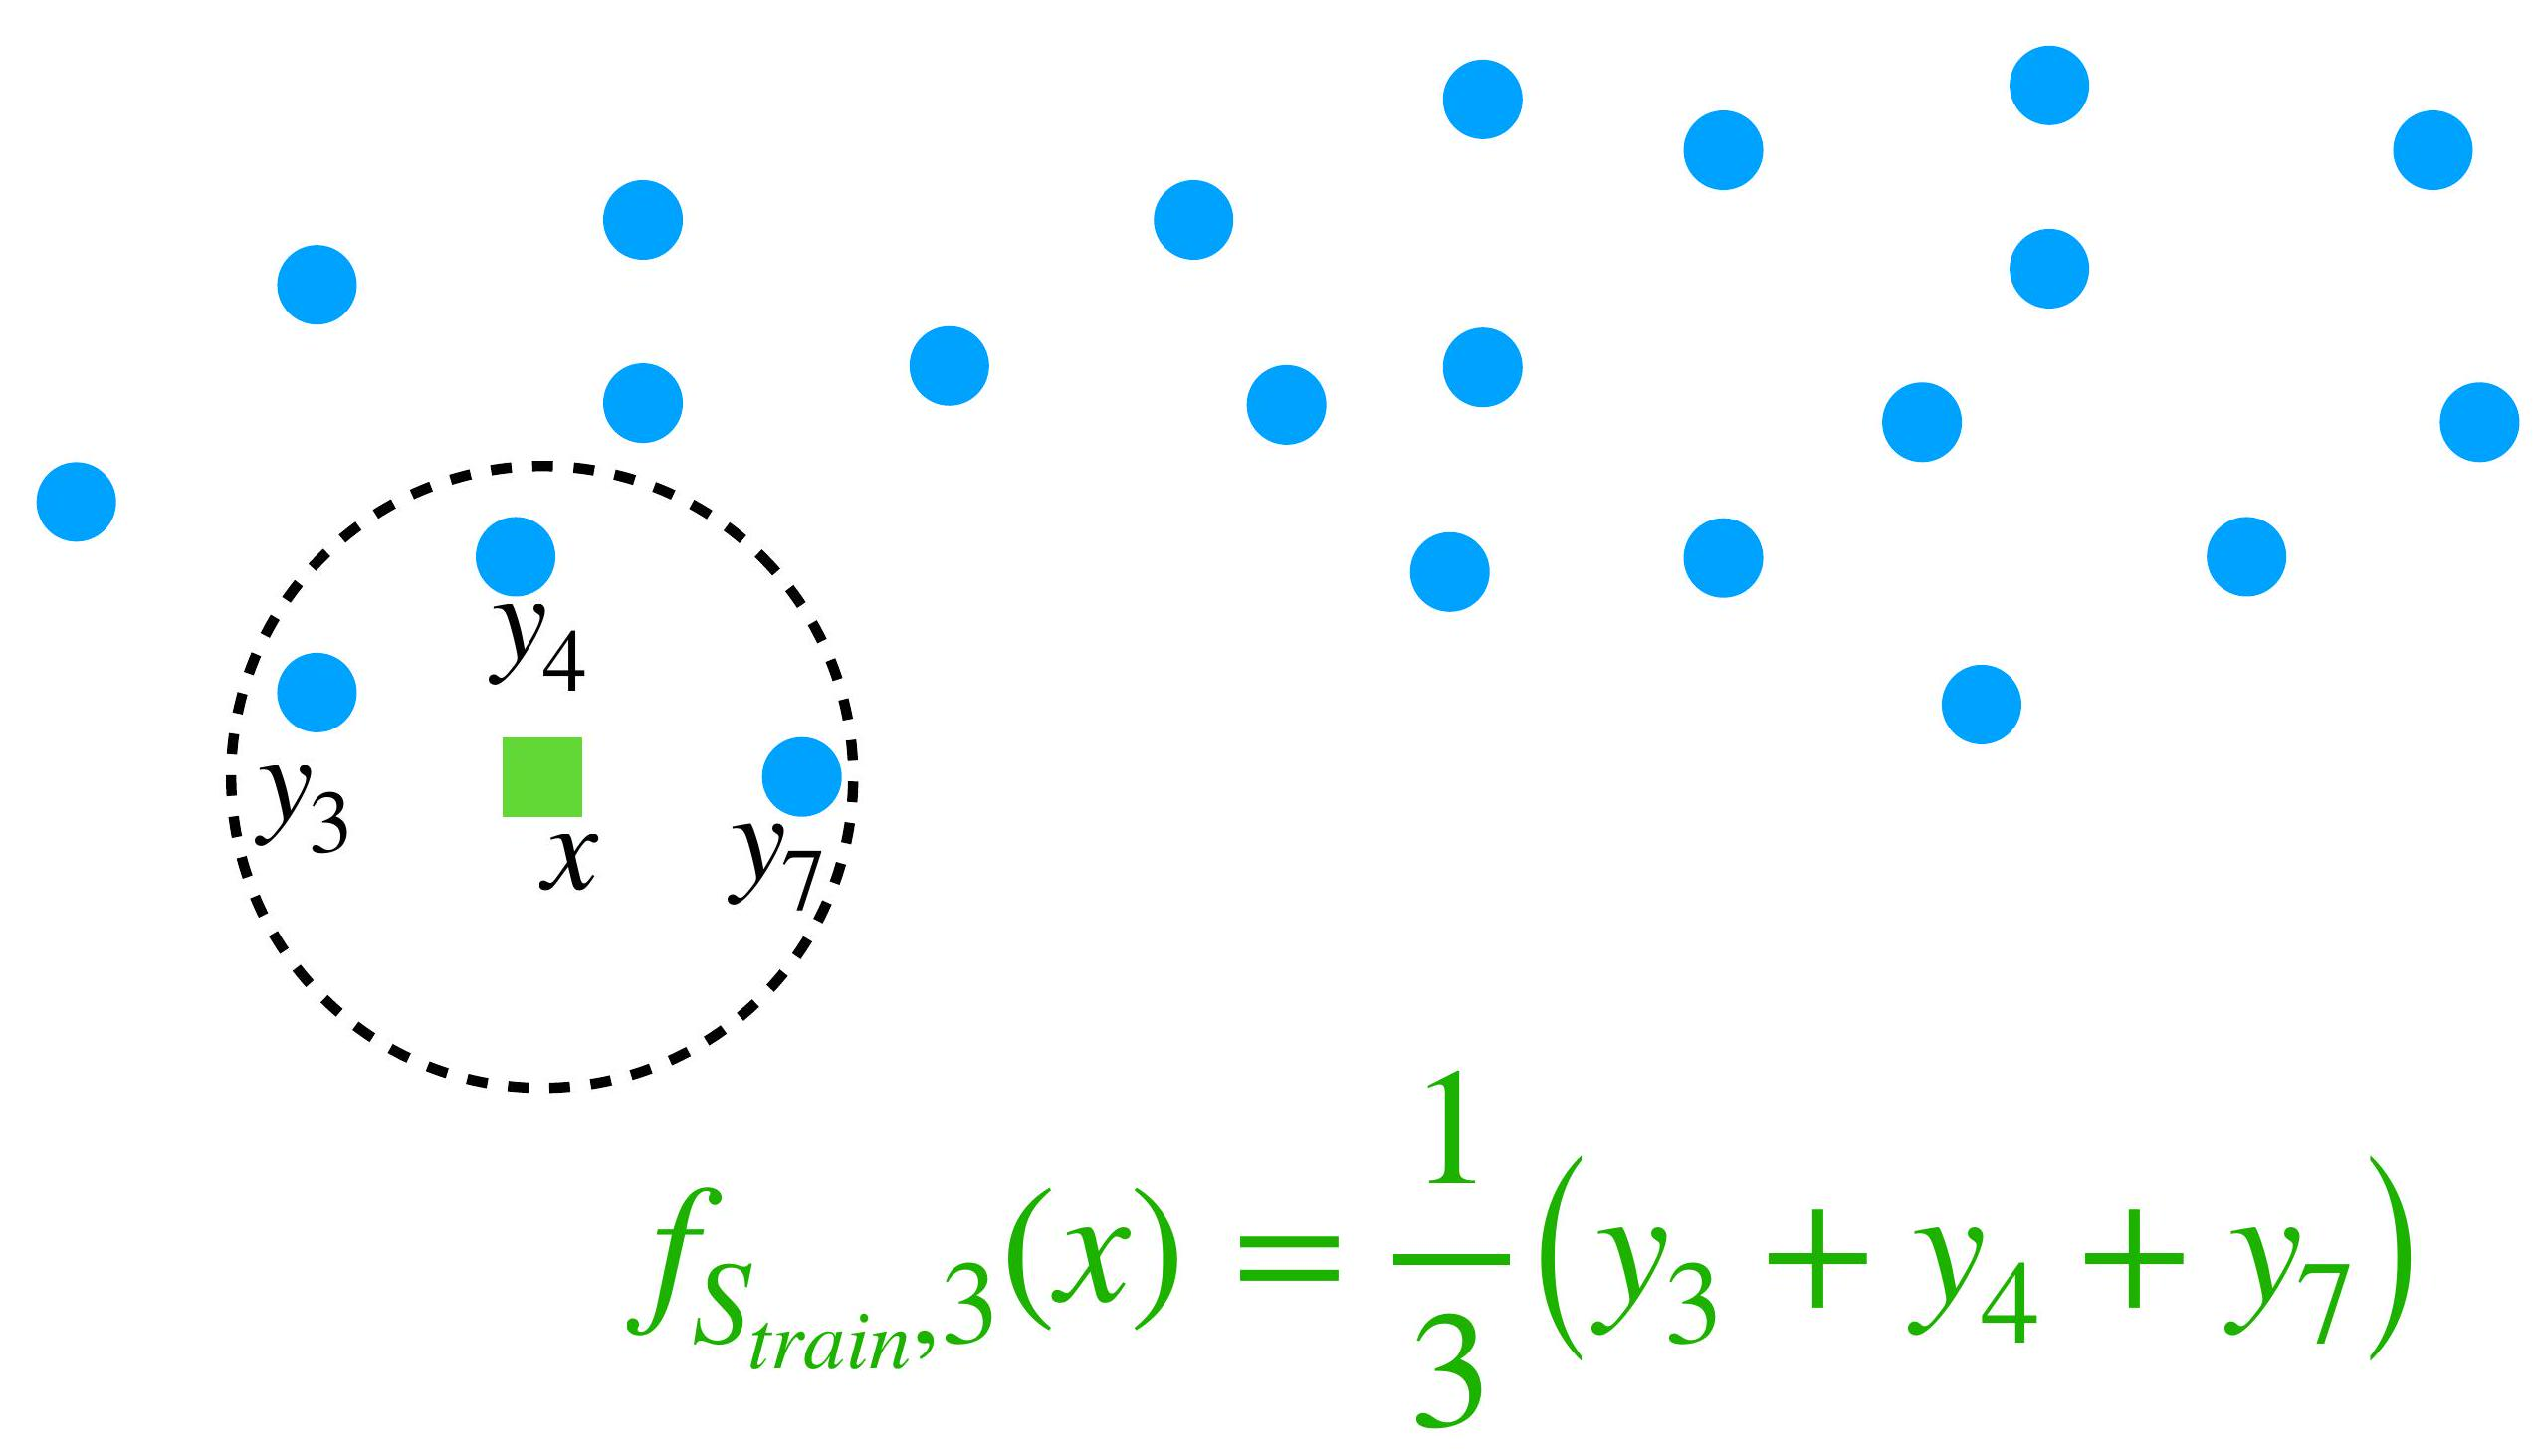
\includegraphics[max width=\textwidth]{2023_12_30_f937b0007b5d87b39f79g-13}
\end{center}

\section*{k-NN can be used for classification $(y \in\{0,1\}$ )}
$$
f_{S_{\text {train }, k}}(x)=\operatorname{majority}\left\{y_{n}: x_{n} \in \operatorname{nbh}_{S_{\text {train }, ~}}(x)\right\}
$$

\begin{center}
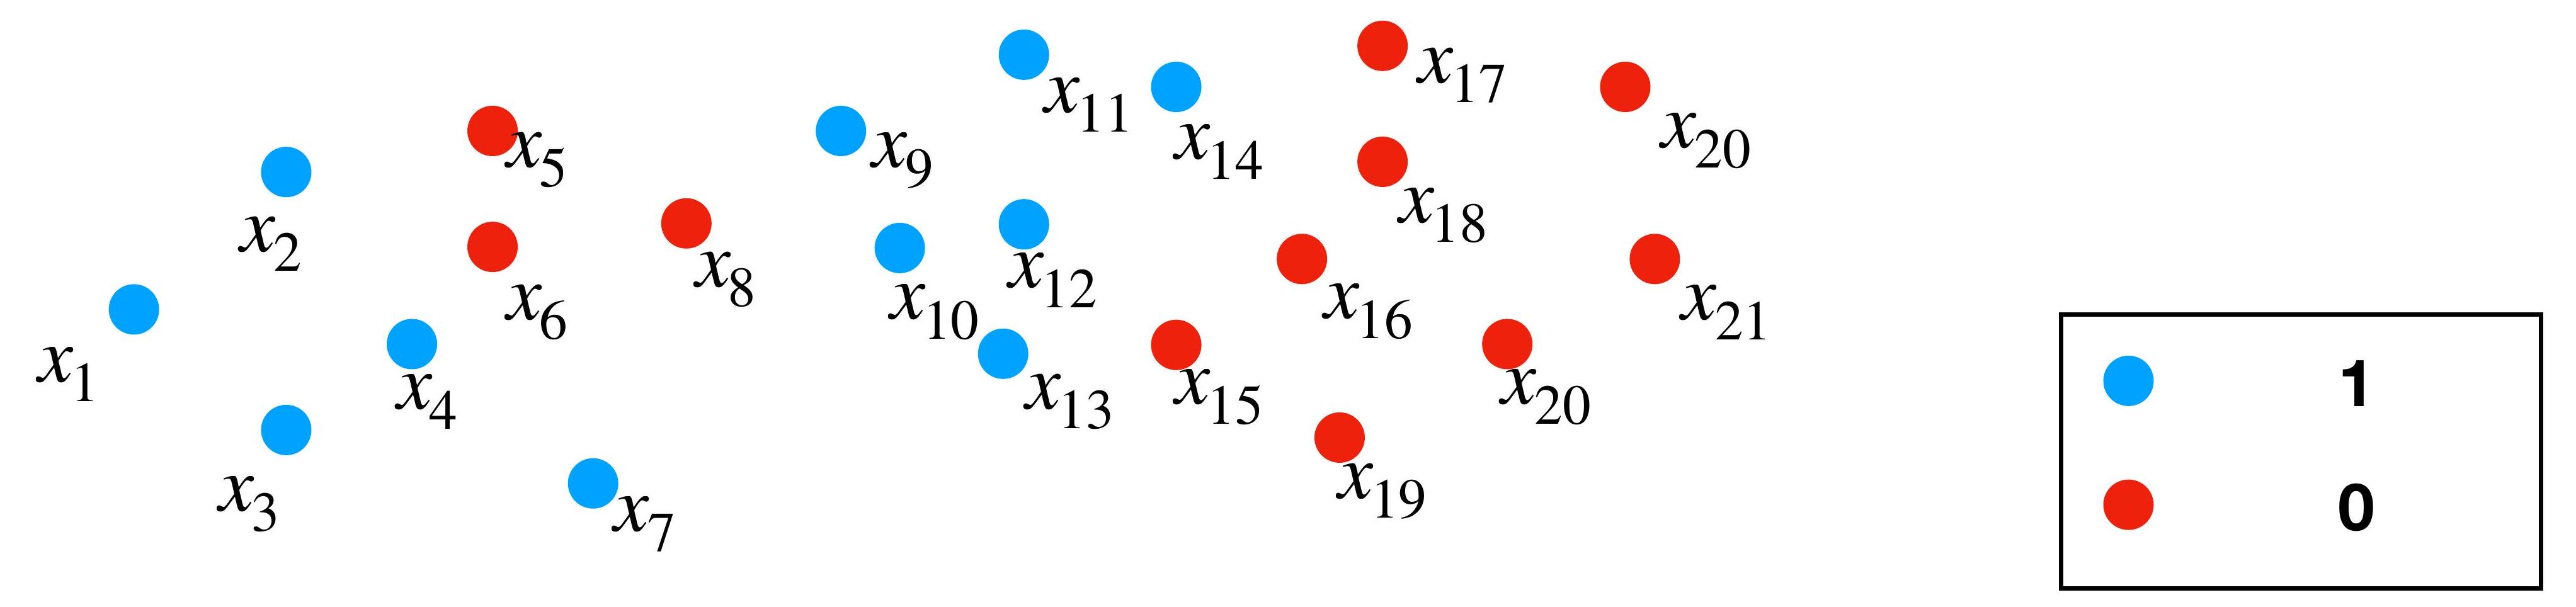
\includegraphics[max width=\textwidth]{2023_12_30_f937b0007b5d87b39f79g-14}
\end{center}

\section*{k-NN can be used for classification $(y \in\{0,1\}$ )}
$$
f_{S_{\text {train }, k}}(x)=\operatorname{majority}\left\{y_{n}: x_{n} \in \operatorname{nbh}_{S_{\text {train }, ~}}(x)\right\}
$$

\begin{center}
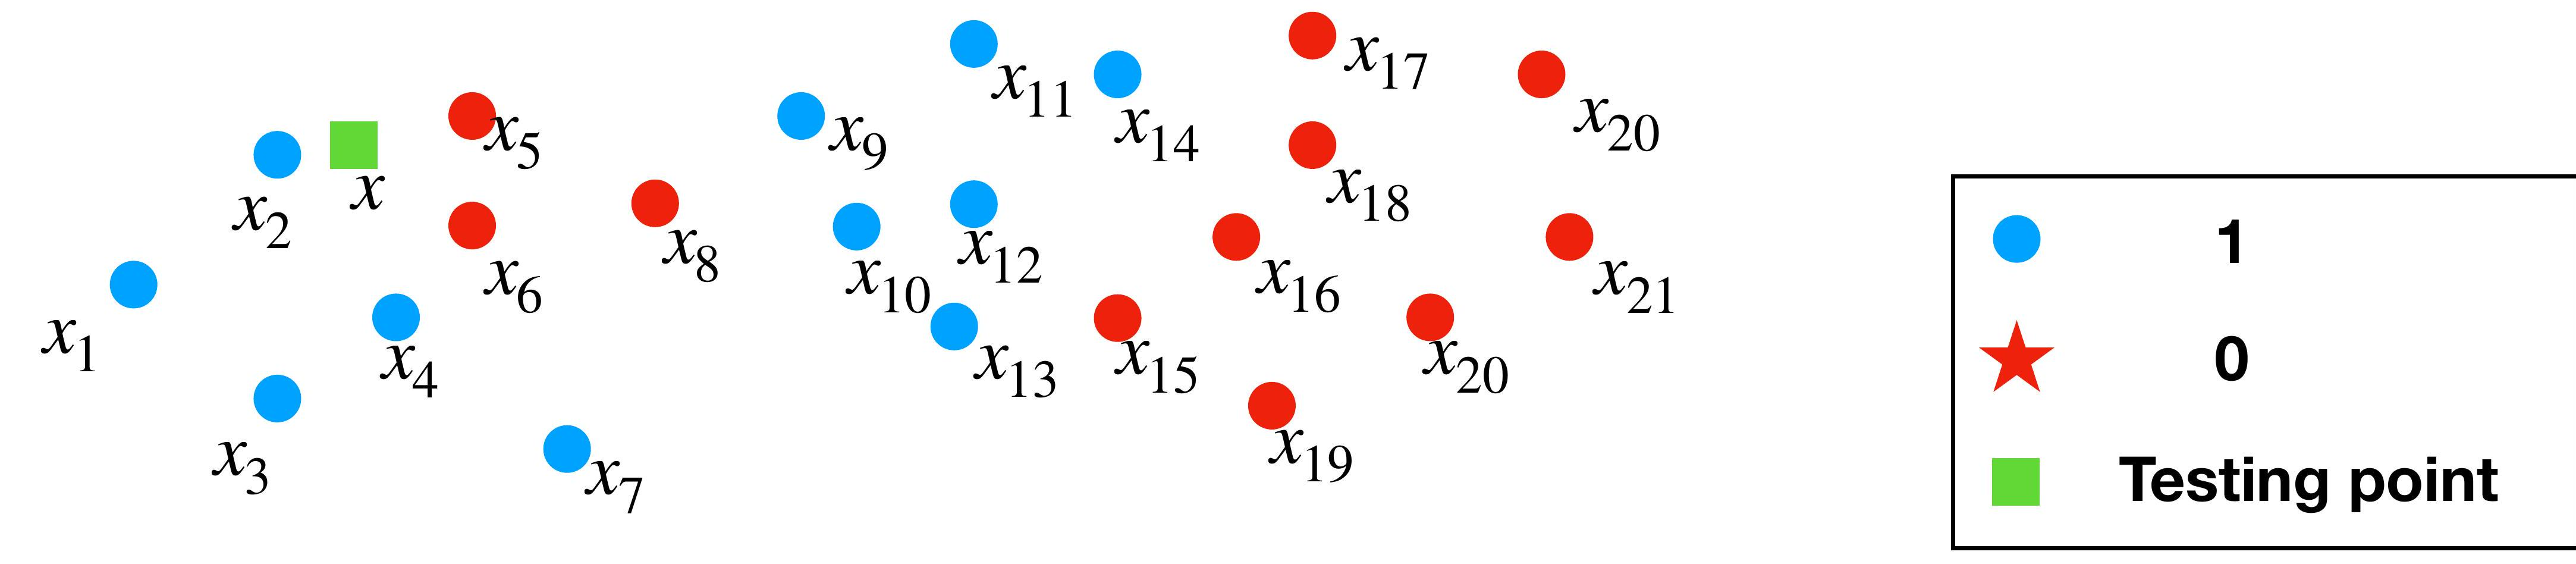
\includegraphics[max width=\textwidth]{2023_12_30_f937b0007b5d87b39f79g-15}
\end{center}

$$
f_{S_{\text {train }, 1}}(x)=?
$$

\section*{k-NN can be used for classification $(y \in\{0,1\}$ )}
$$
f_{S_{\text {train }, k}}(x)=\operatorname{majority}\left\{y_{n}: x_{n} \in \operatorname{nbh}_{S_{\text {train }, ~}}(x)\right\}
$$

\begin{center}
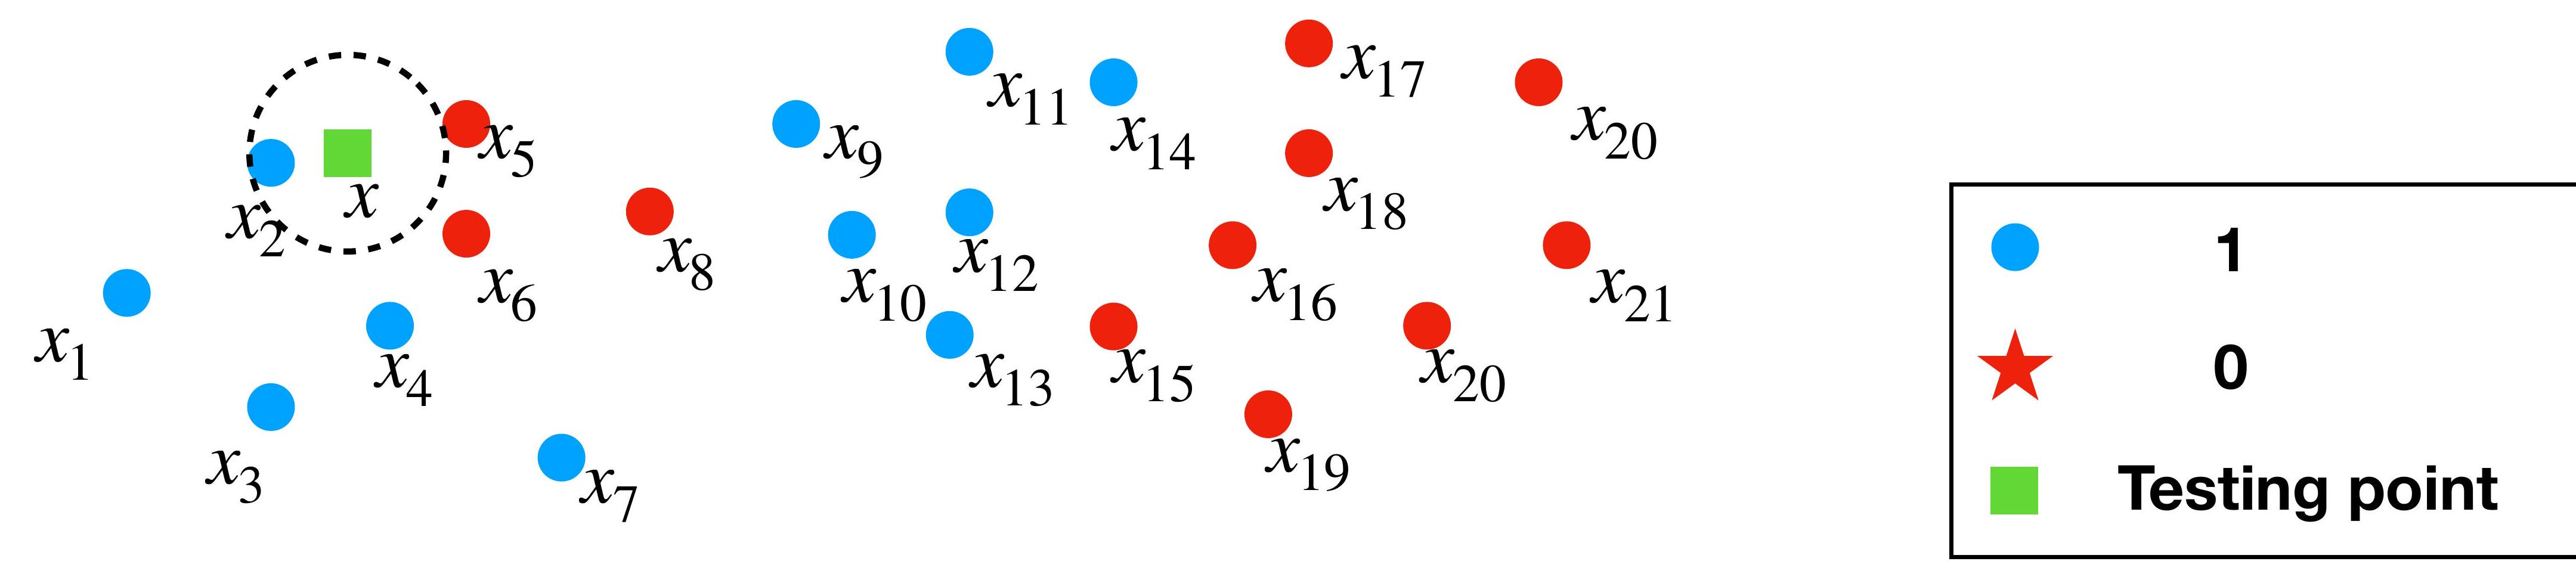
\includegraphics[max width=\textwidth]{2023_12_30_f937b0007b5d87b39f79g-16}
\end{center}

$$
f_{S_{\text {train } 1}}(x)=1
$$

\section*{k-NN can be used for classification $(y \in\{0,1\}$ )}
$$
f_{S_{\text {train }, k}}(x)=\operatorname{majority}\left\{y_{n}: x_{n} \in \operatorname{nbh}_{S_{\text {train }, ~}}(x)\right\}
$$

\begin{center}
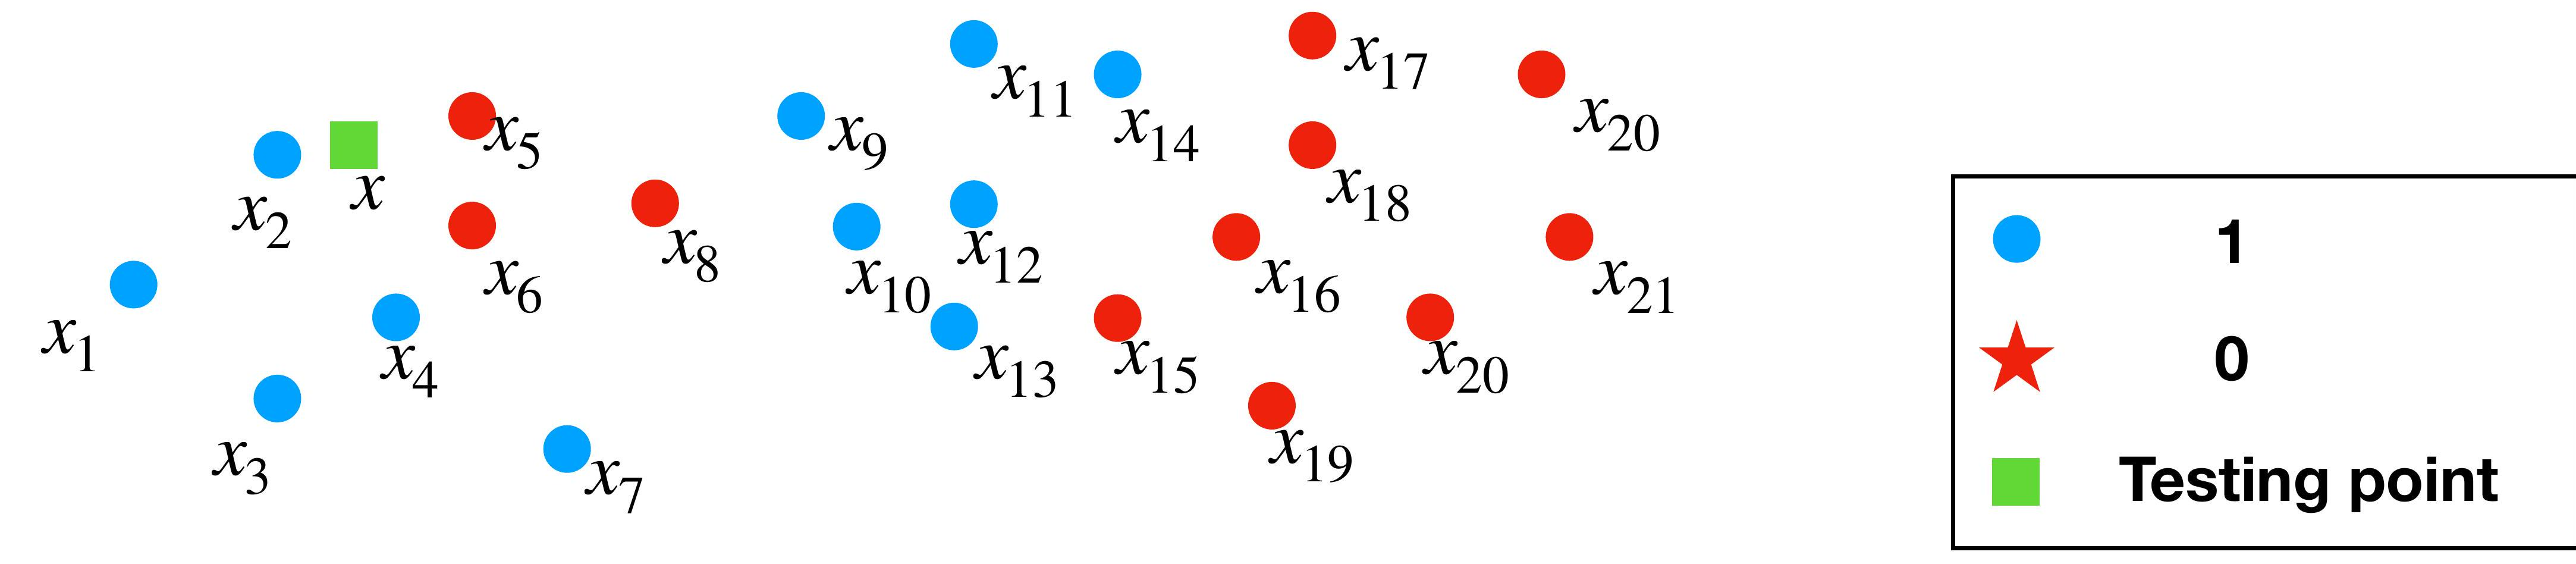
\includegraphics[max width=\textwidth]{2023_12_30_f937b0007b5d87b39f79g-17}
\end{center}

$$
f_{S_{\text {train } 3}}(x)=?
$$

\section*{k-NN can be used for classification $(y \in\{0,1\}$ )}
$$
f_{S_{\text {train }, k}}(x)=\operatorname{majority}\left\{y_{n}: x_{n} \in \operatorname{nbh}_{S_{\text {train }, ~}}(x)\right\}
$$

\begin{center}
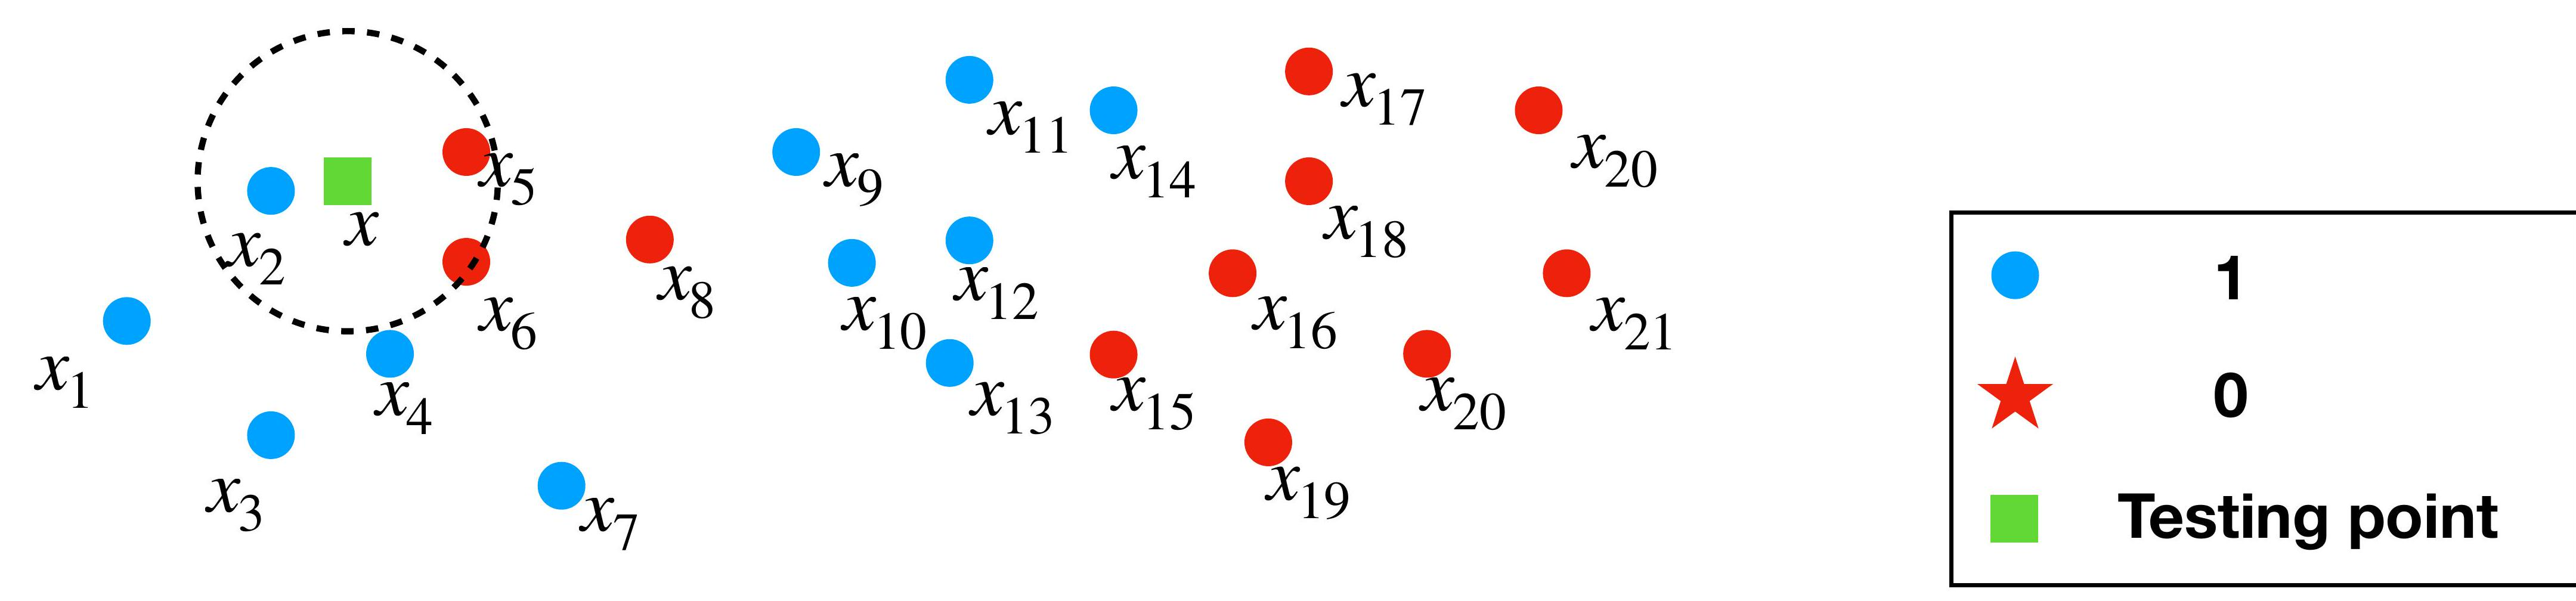
\includegraphics[max width=\textwidth]{2023_12_30_f937b0007b5d87b39f79g-18}
\end{center}

$$
f_{S_{\text {train } 3}}(x)=0
$$

\section*{k-NN can be used for classification $(y \in\{0,1\}$ )}
$$
f_{S_{\text {train }, k}}(x)=\operatorname{majority}\left\{y_{n}: x_{n} \in \operatorname{nbh}_{S_{\text {train }, ~}}(x)\right\}
$$

\begin{center}
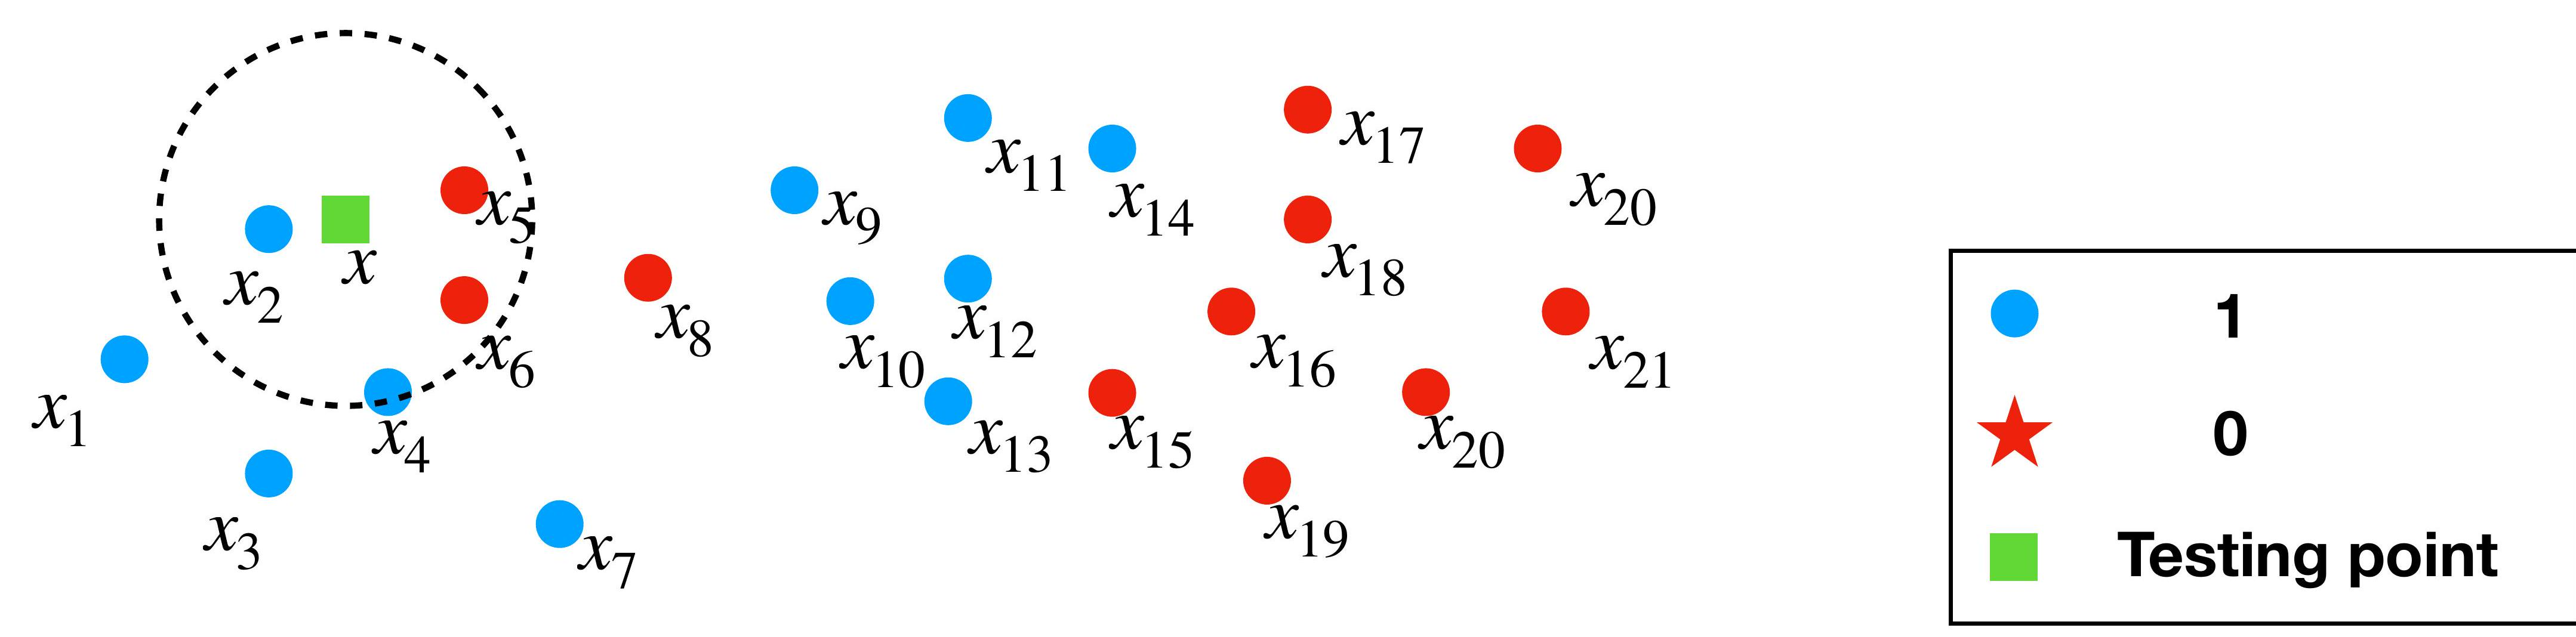
\includegraphics[max width=\textwidth]{2023_12_30_f937b0007b5d87b39f79g-19}
\end{center}

$$
f_{S_{\text {train } 4}}(x)=? \text { Tie! }
$$

\section*{k-NN can be used for classification $(y \in\{0,1\})$}
$$
f_{S_{\text {train }, k}}(x)=\text { majority }\left\{y_{n}: x_{n} \in \operatorname{nbh}_{S_{\text {train }}, k}(x)\right\}
$$

\begin{center}
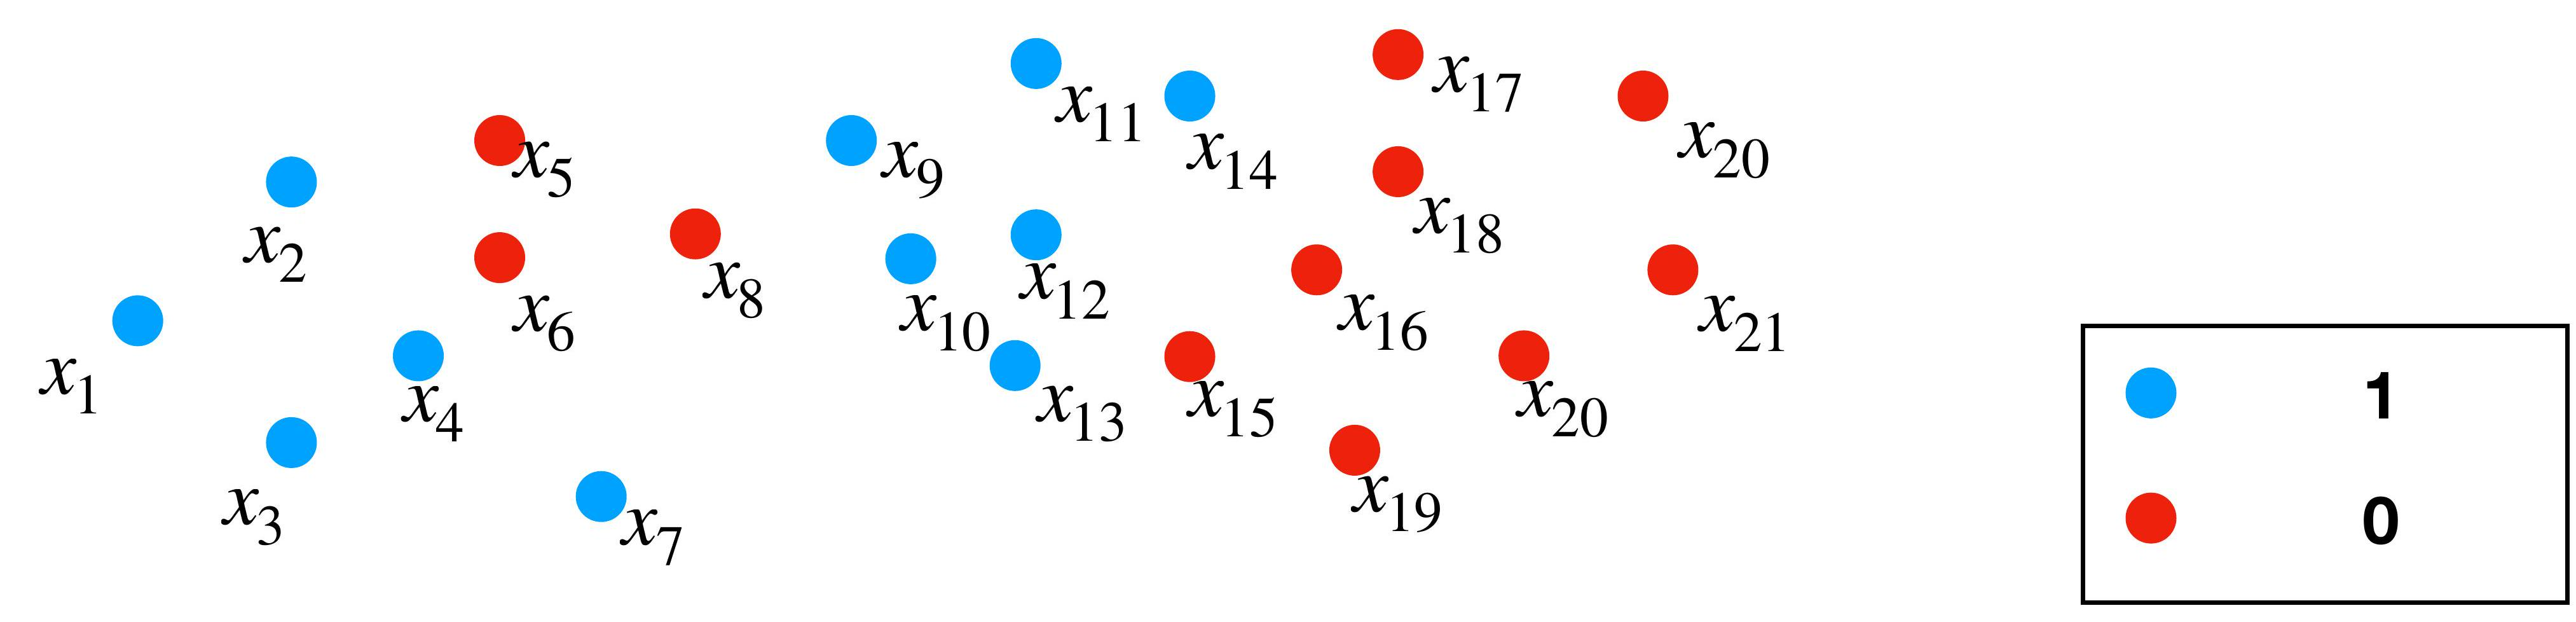
\includegraphics[max width=\textwidth]{2023_12_30_f937b0007b5d87b39f79g-20}
\end{center}

Remarks:

\begin{itemize}
  \item Choose an odd value for $\mathrm{k}$ to prevent ties
  \item Generalization: smoothing kernels; weighted linear combination of elements
\end{itemize}

\section*{Why does it make sense?}
\begin{itemize}
  \item Relevant in the presence of spatial correlation

  \item Implicitly models intricate decision boundaries in low-dimensional spaces

\end{itemize}

\begin{center}
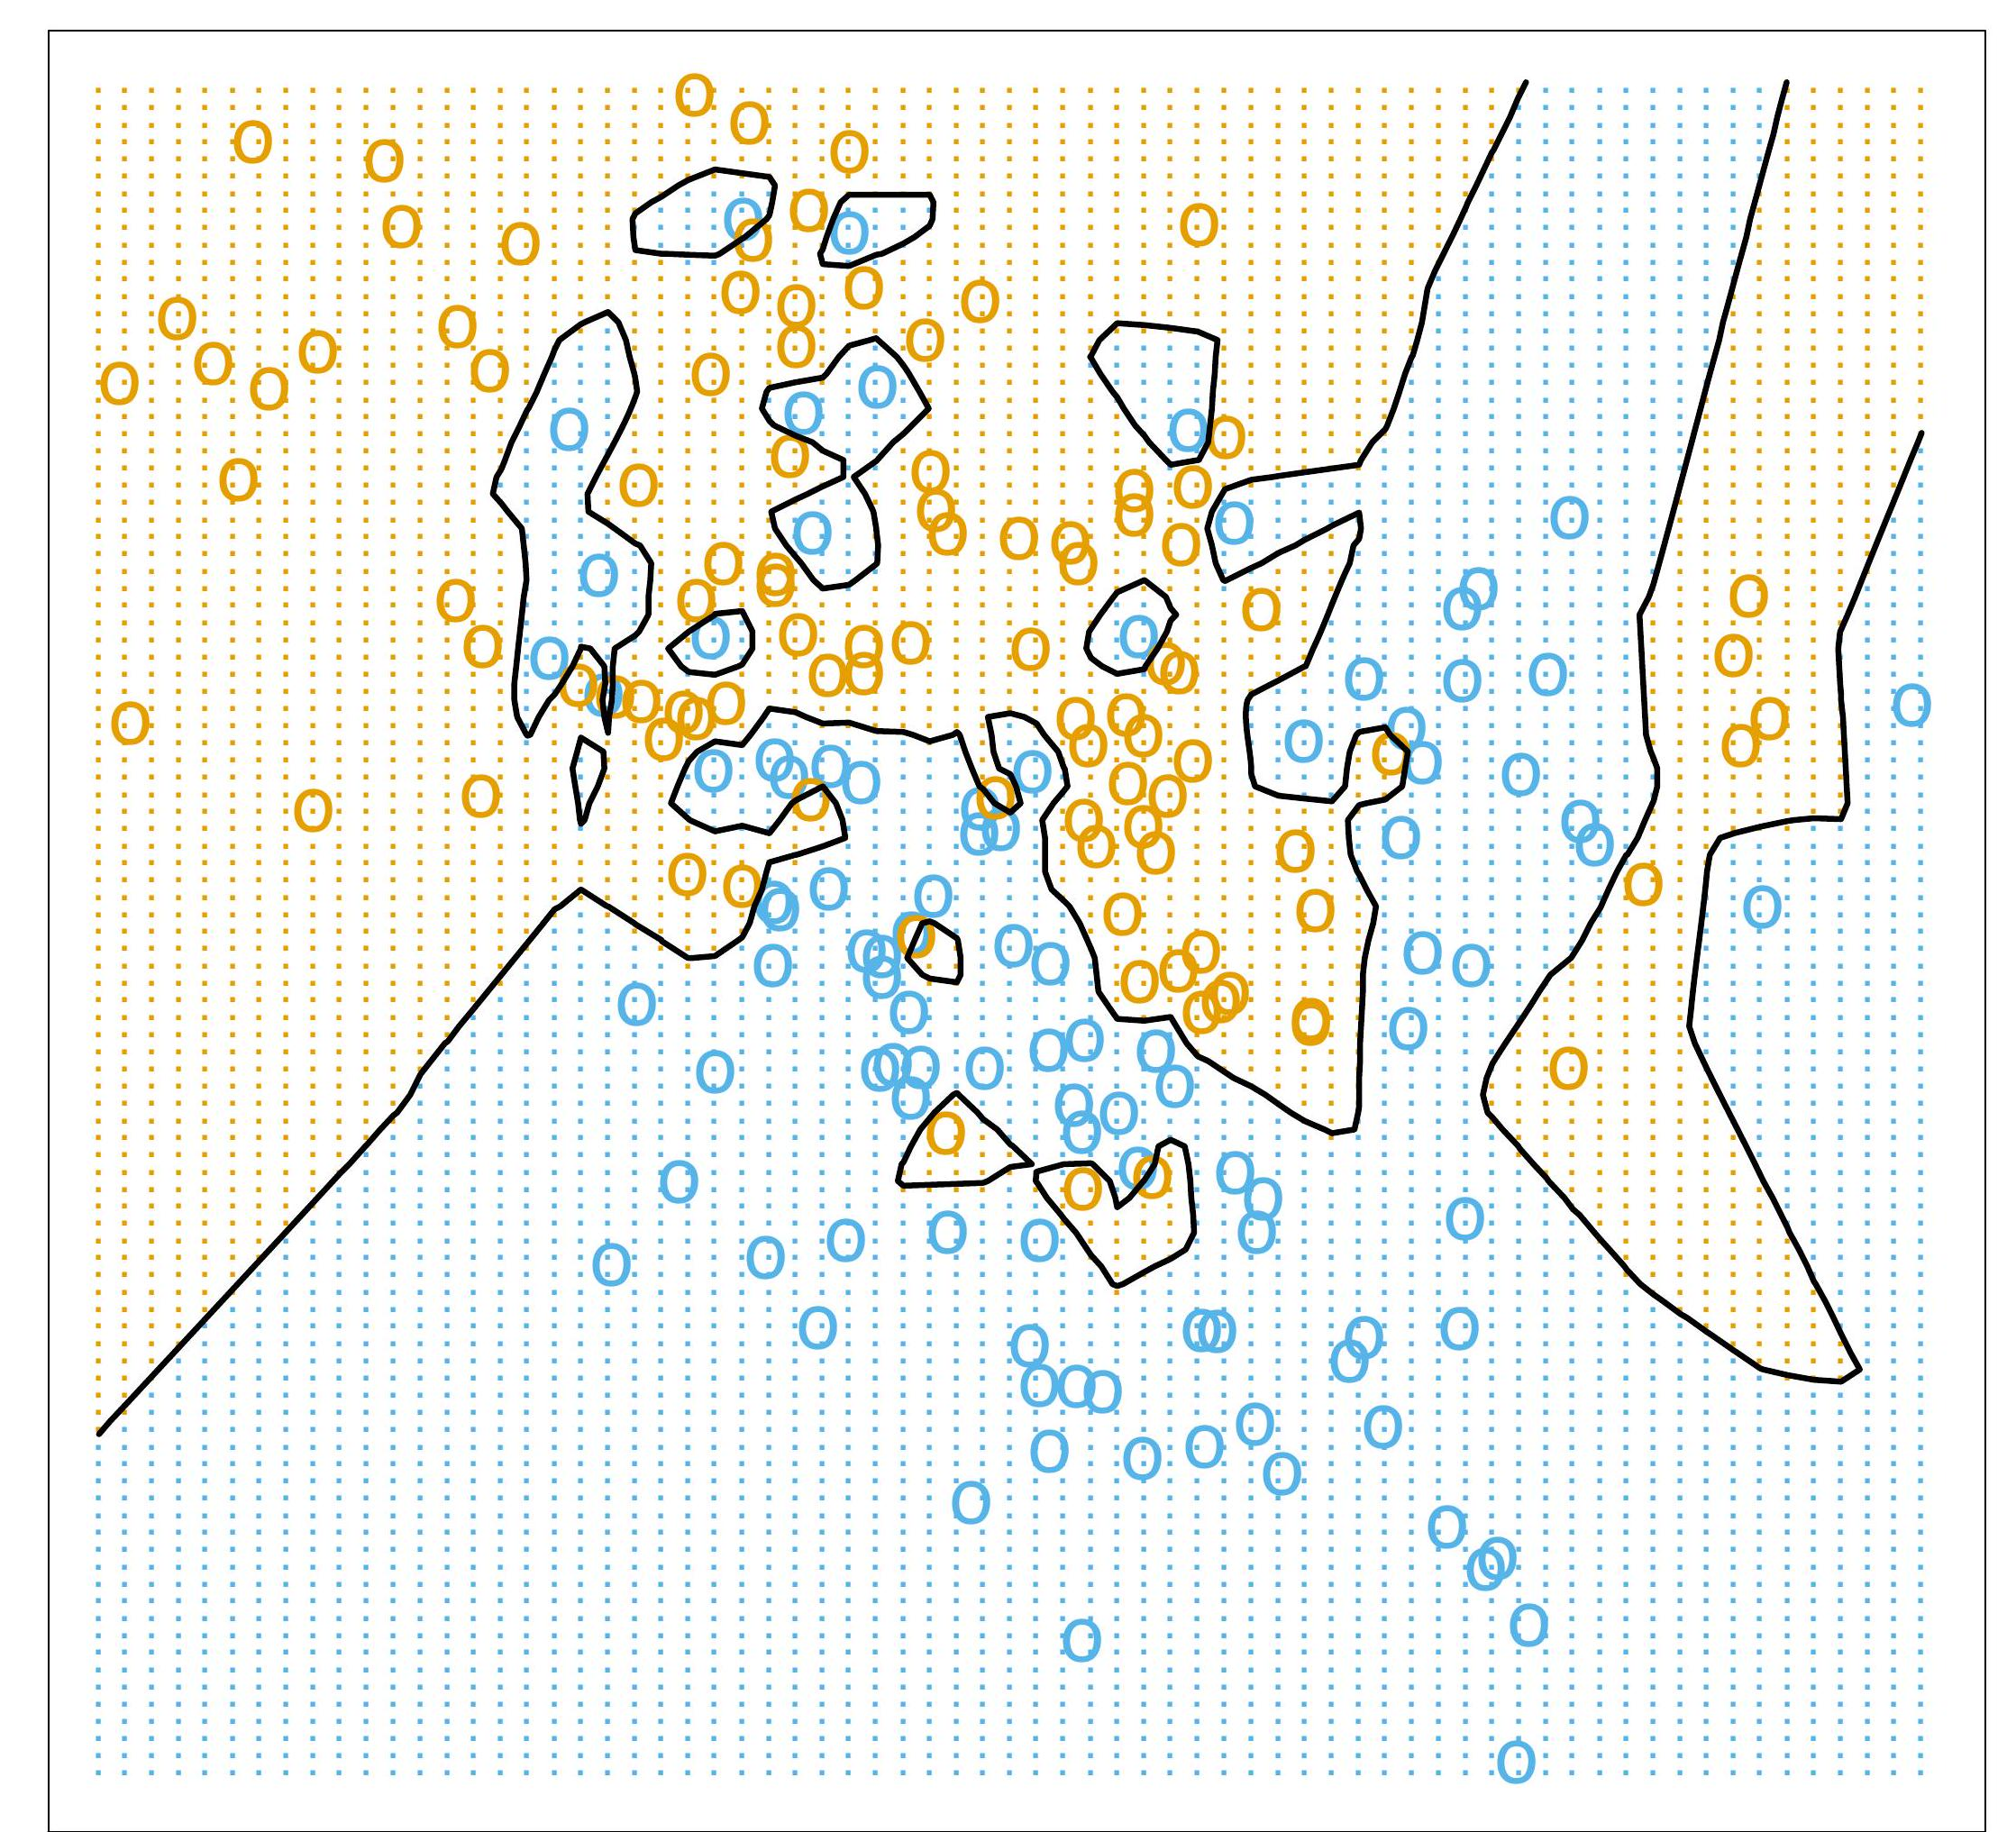
\includegraphics[max width=\textwidth]{2023_12_30_f937b0007b5d87b39f79g-21}
\end{center}

\section*{Bias-variance tradeoff in k-NN}
For small k:

\begin{itemize}
  \item Low bias - complex decision boundary
  \item High variance - overfitting
\end{itemize}

For large k:

(When $k=N$, prediction is constant)

\begin{itemize}
  \item High bias
  \item Low variance
\end{itemize}

\begin{center}
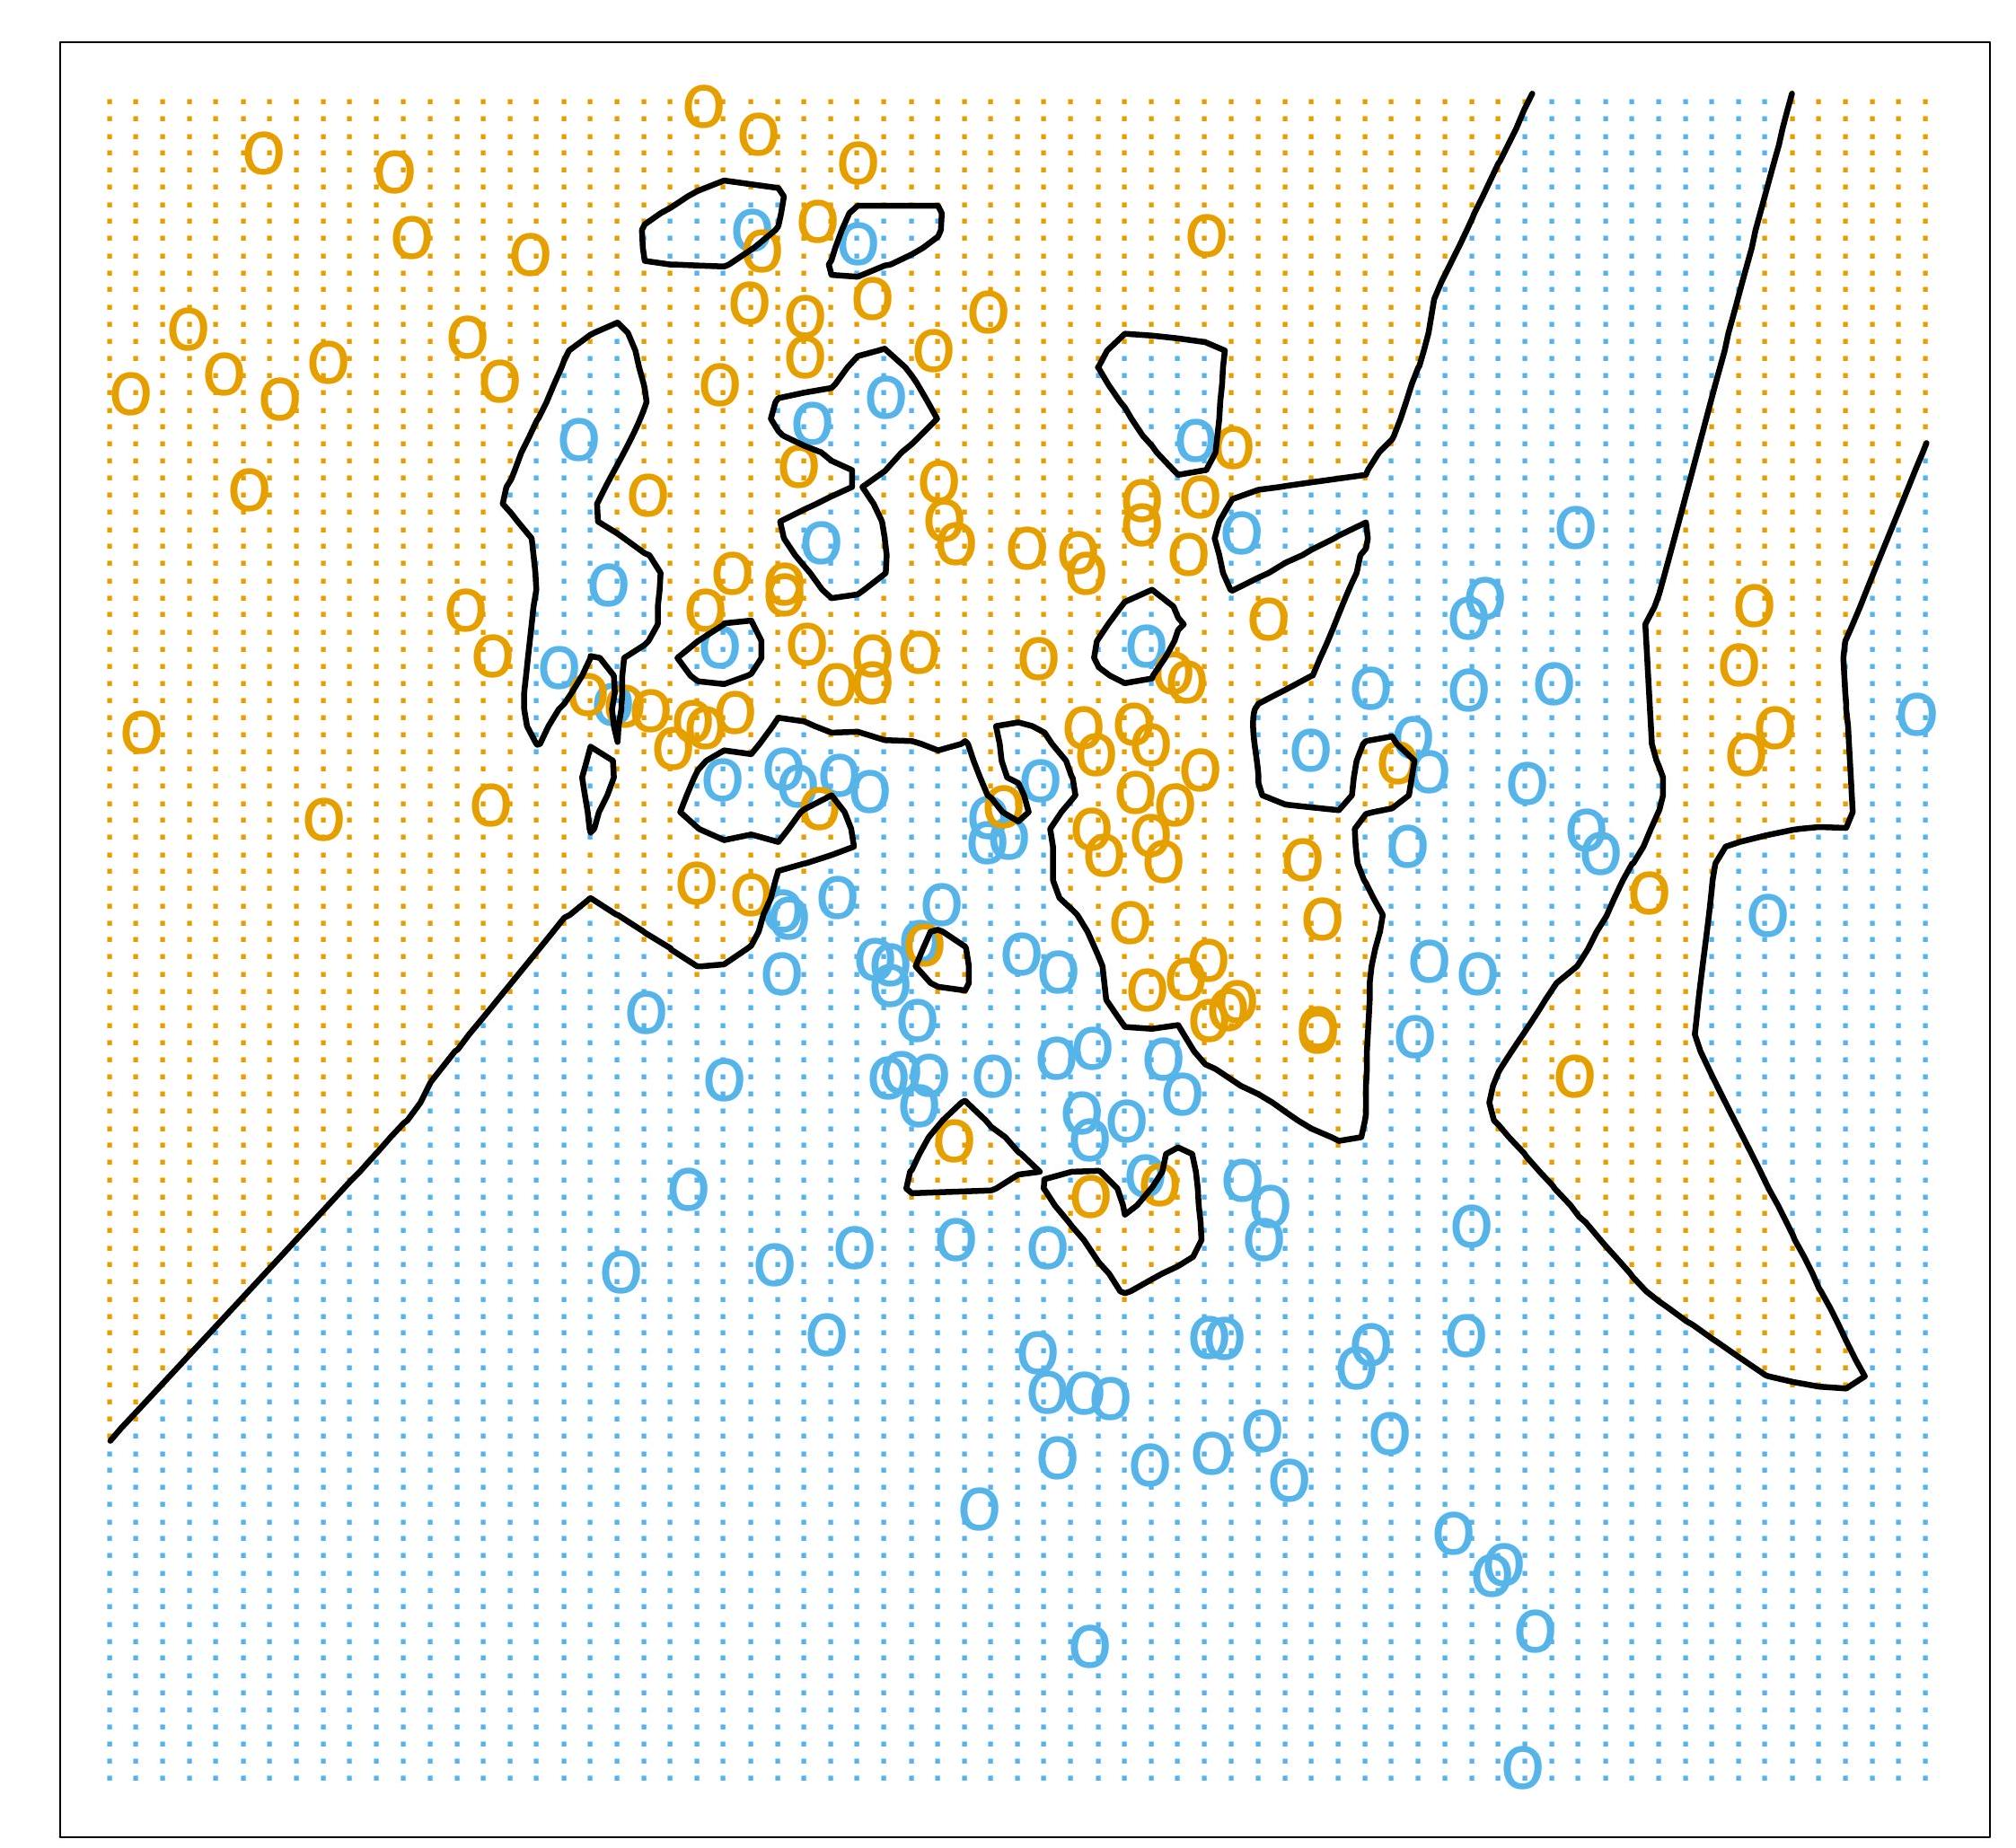
\includegraphics[max width=\textwidth]{2023_12_30_f937b0007b5d87b39f79g-22}
\end{center}

1-nearest neighbor classification

\section*{U-shaped curve for $\mathrm{k}-\mathrm{NN}$ bias-variance tradeoff}
\begin{center}
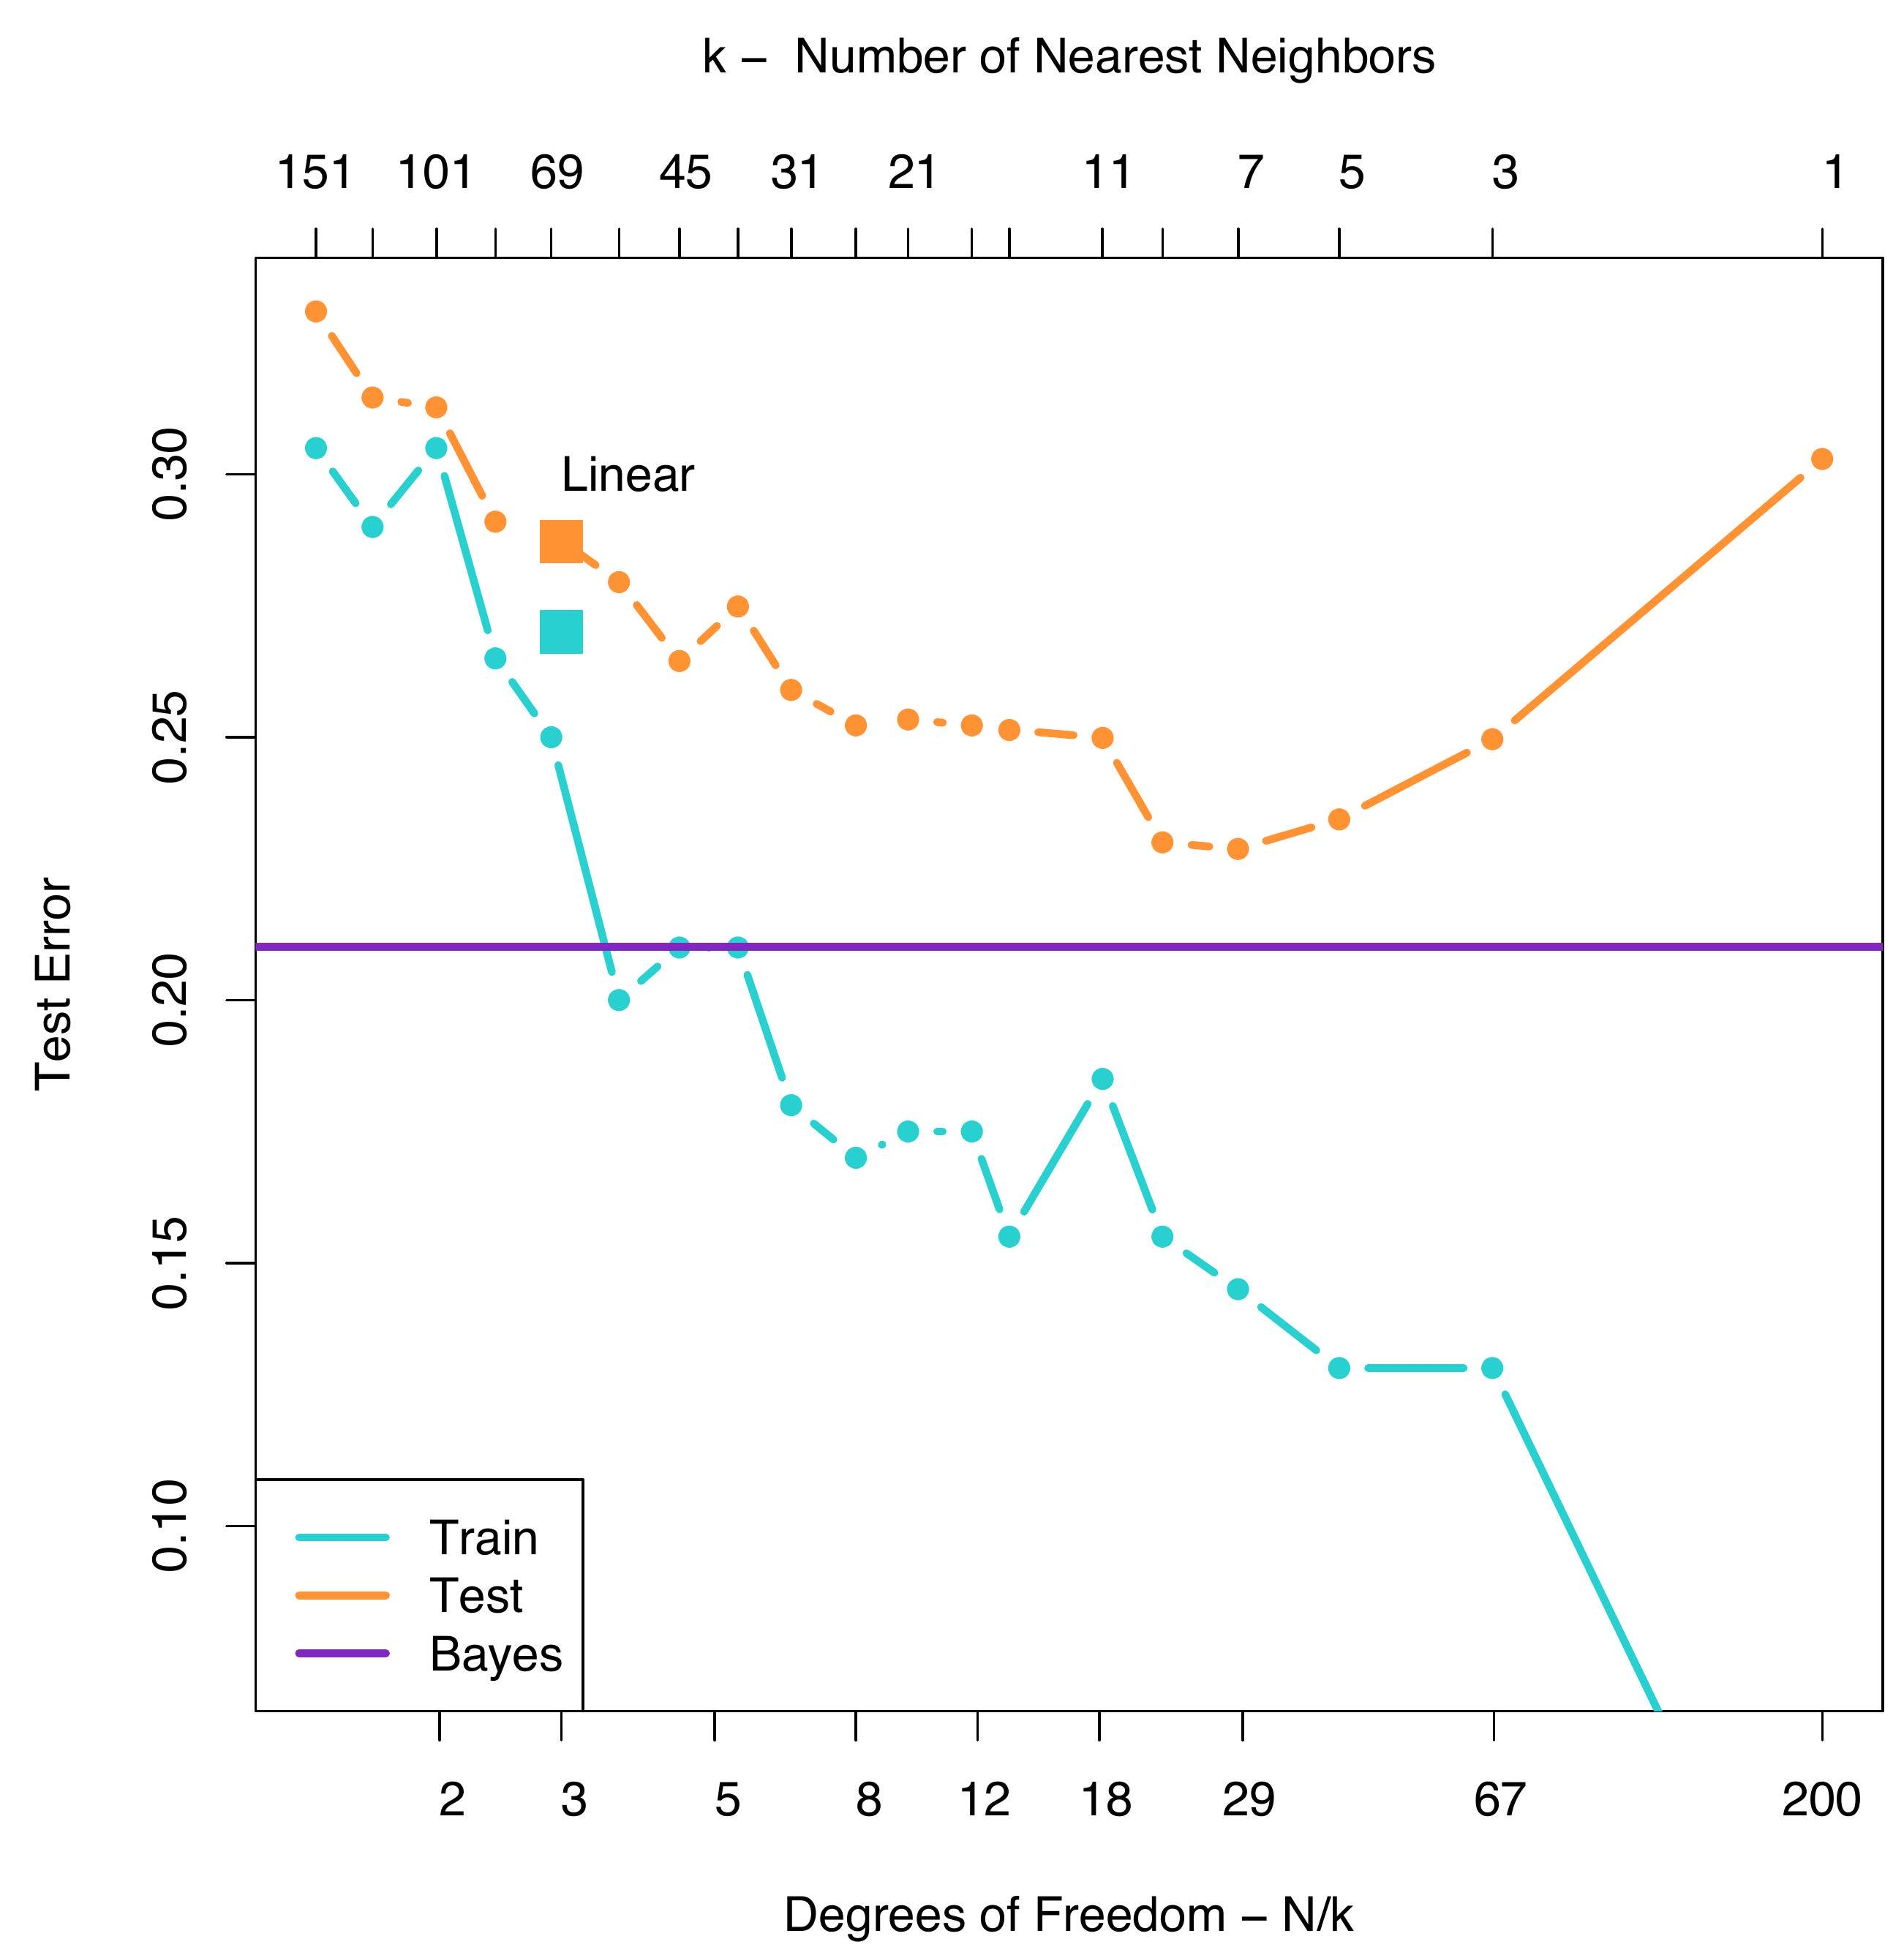
\includegraphics[max width=\textwidth]{2023_12_30_f937b0007b5d87b39f79g-23}
\end{center}

Complexity increases as $k$ decreases

\section*{Find a $k$ that balances bias and variance}
Characteristics of an optimal k:

\begin{itemize}
  \item Low bias: Ensures a sufficiently complex decision boundary
  \item Low variance: Prevents overfitting
\end{itemize}

\begin{center}
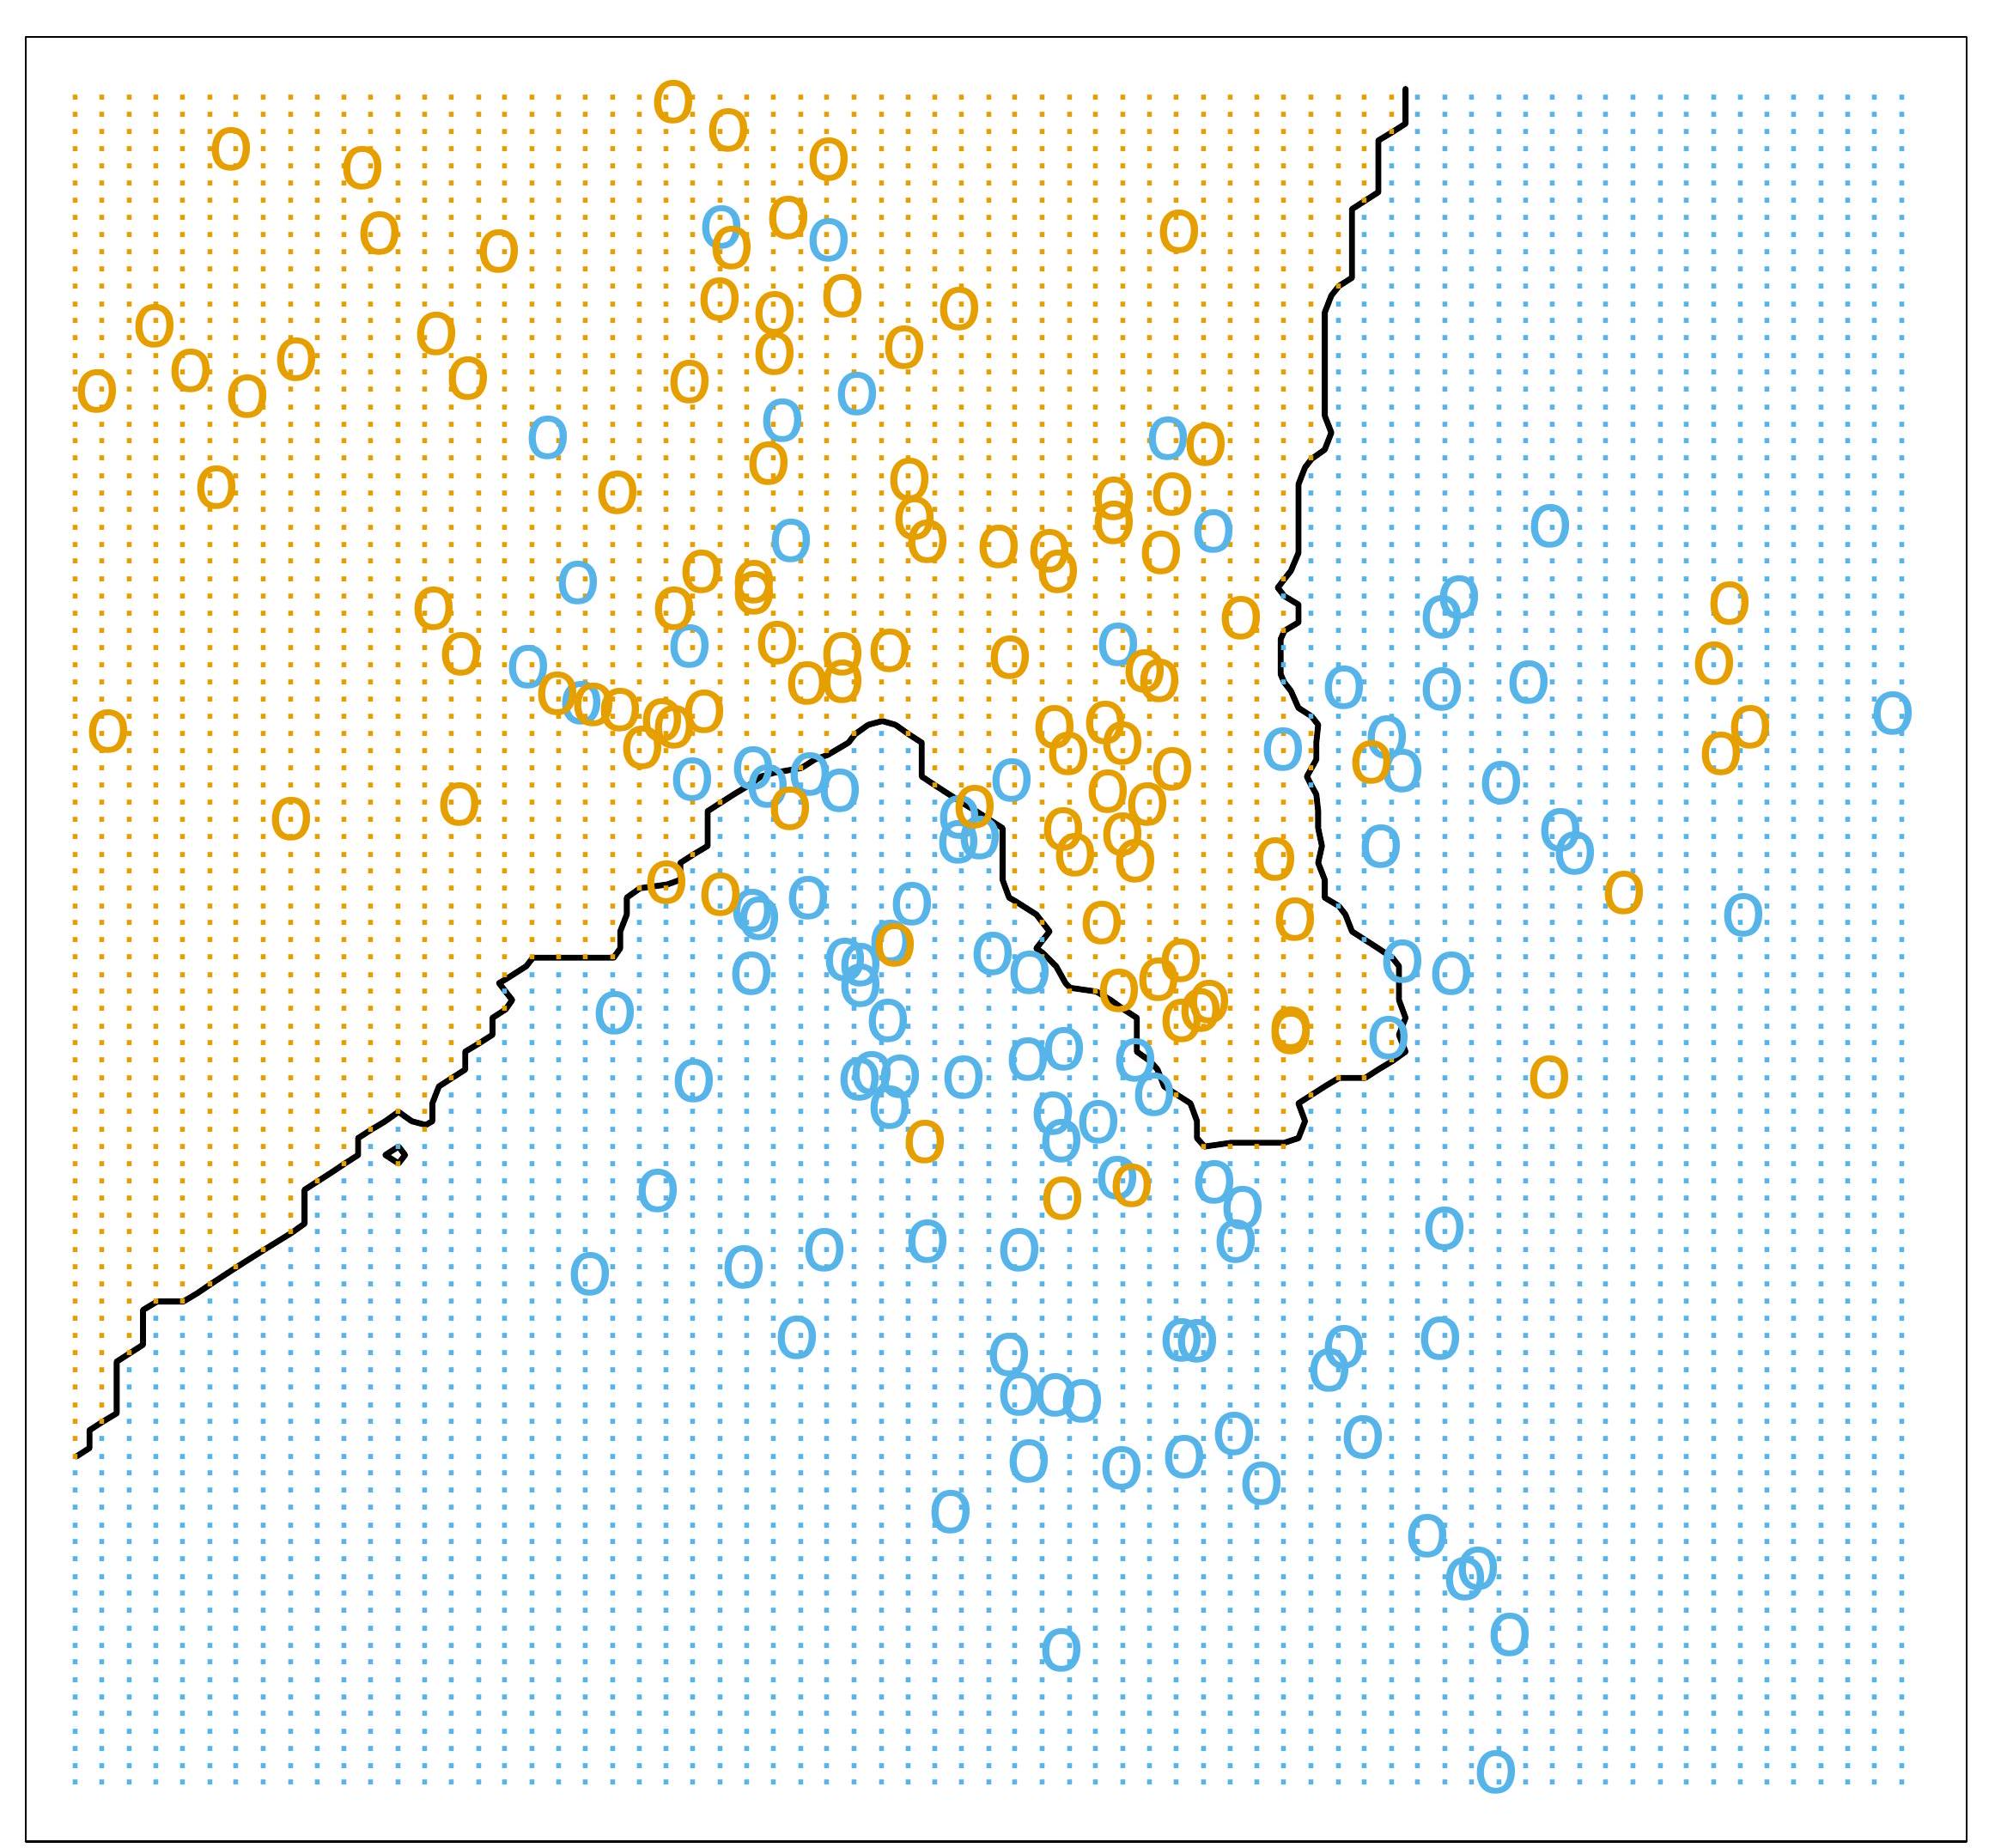
\includegraphics[max width=\textwidth]{2023_12_30_f937b0007b5d87b39f79g-24}
\end{center}

\section*{Summary: k-Nearest Neighbor}
\section*{Pros:}
\begin{itemize}
  \item No optimization or training
  \item Easy to implement
  \item Works well in low dimensions, allowing for very complex decision boundaries
\end{itemize}

Cons:

\begin{itemize}
  \item Slow at query time
  \item Not suitable for high-dimensional data
  \item Choosing the right local distance is crucial
\end{itemize}

\begin{center}
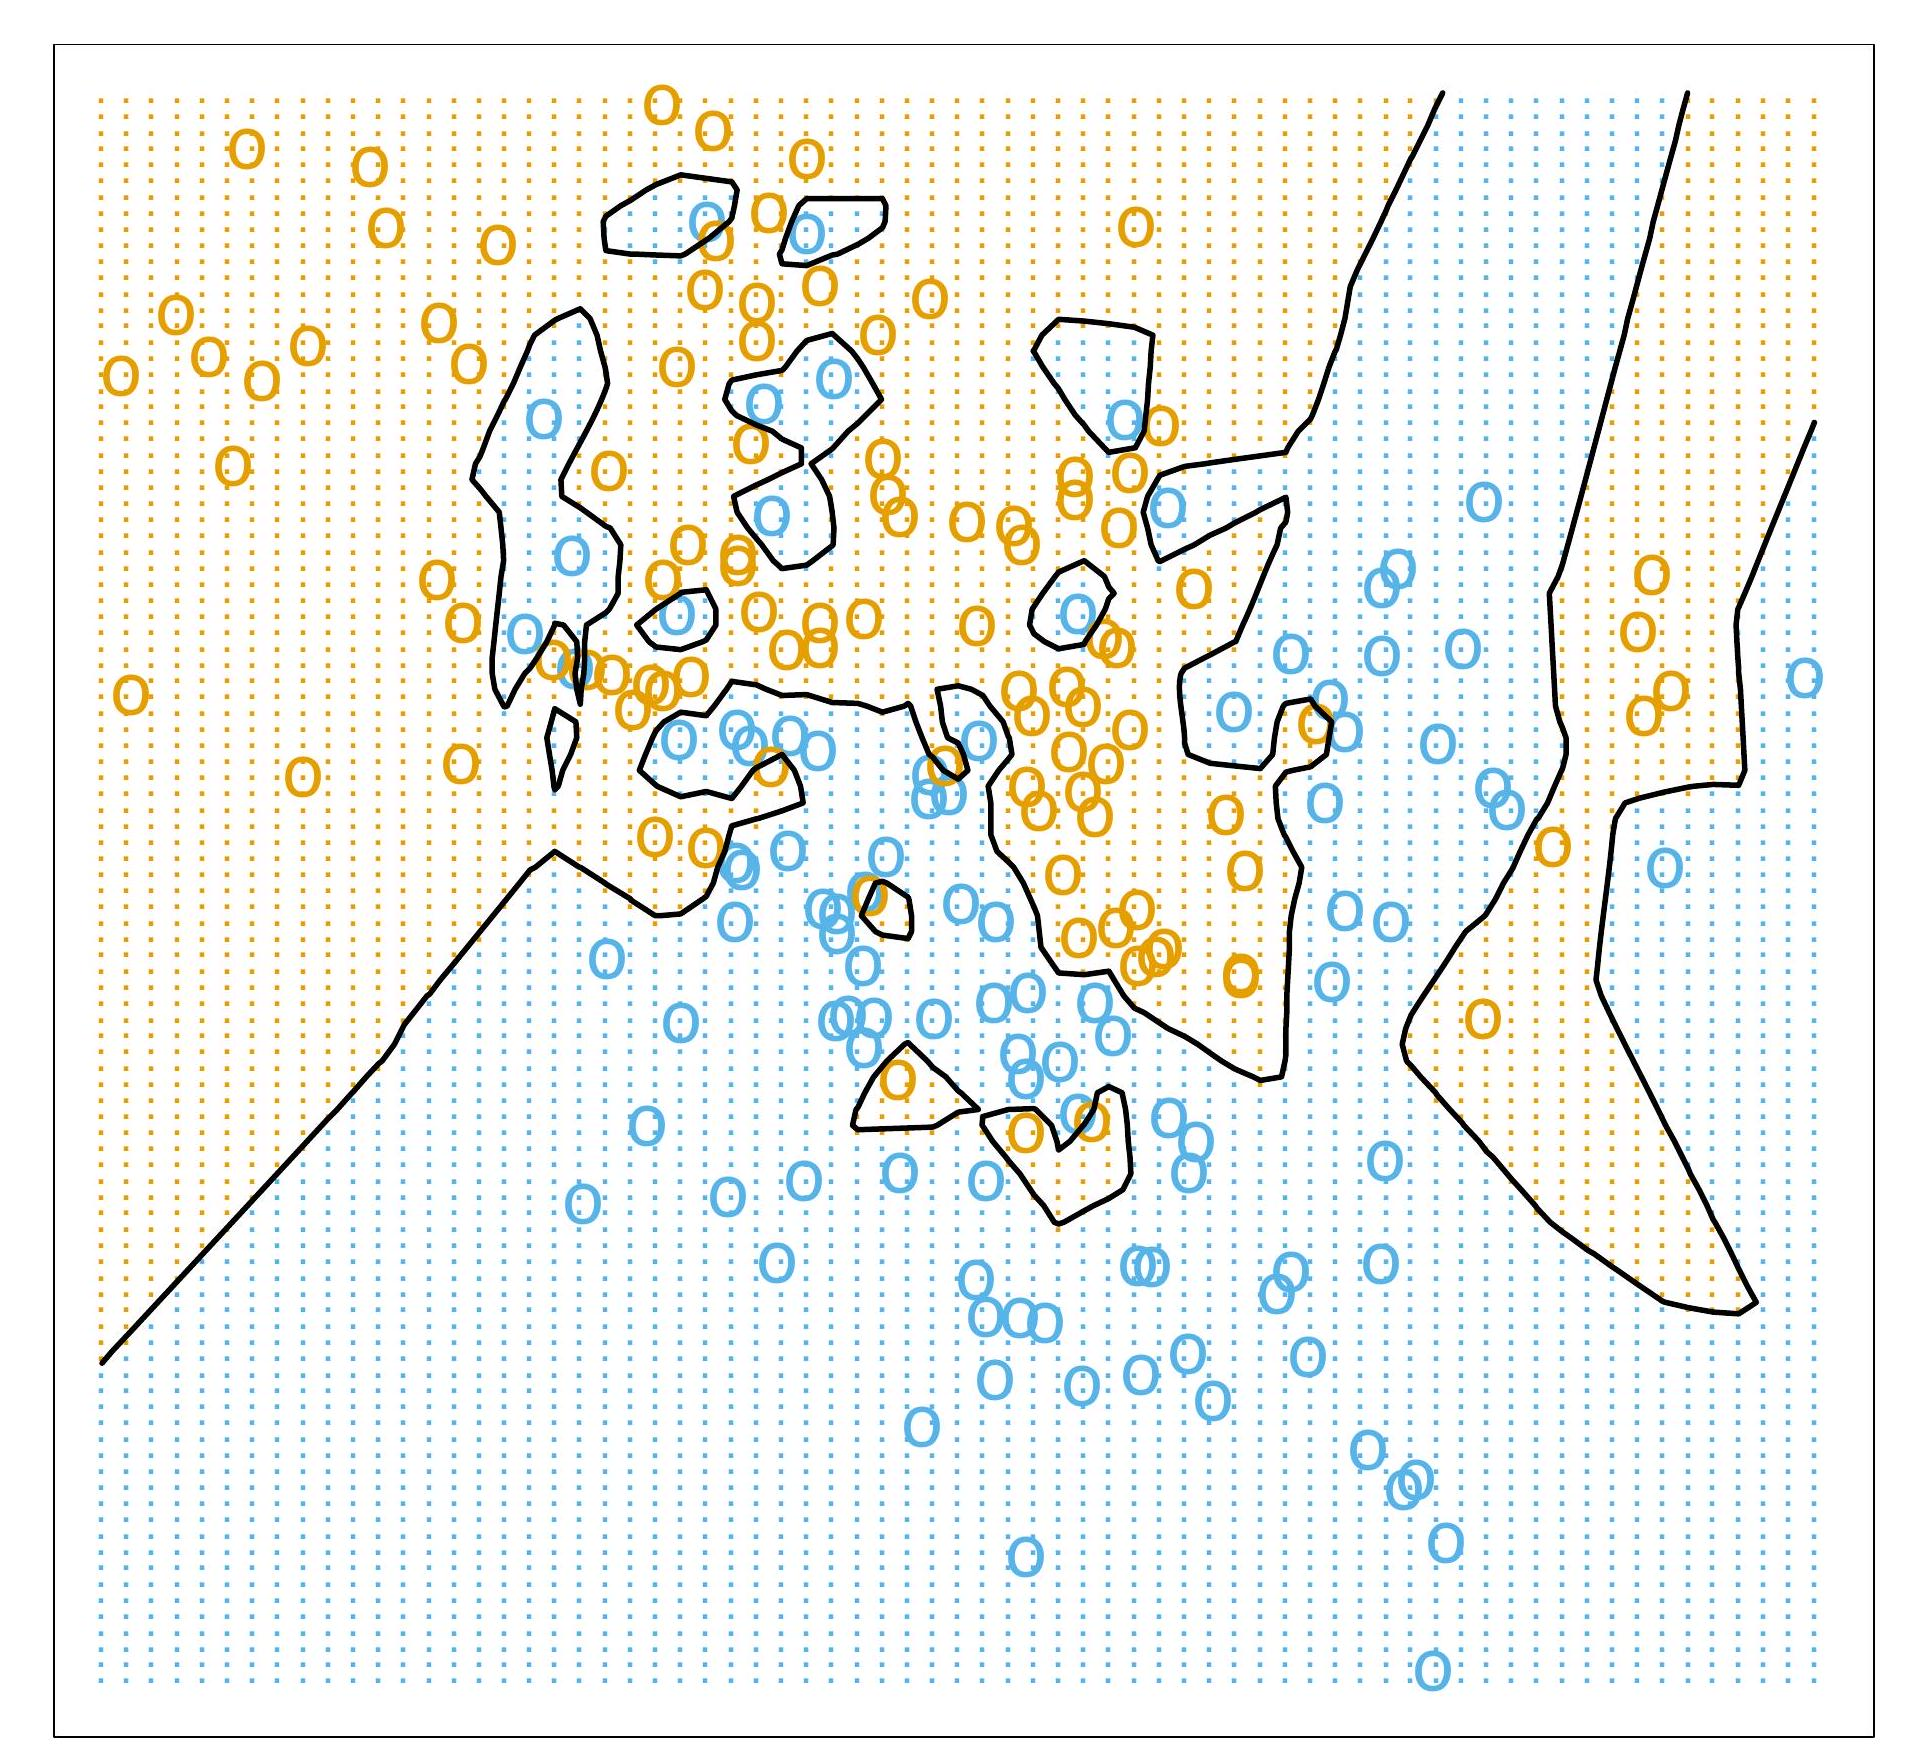
\includegraphics[max width=\textwidth]{2023_12_30_f937b0007b5d87b39f79g-25}
\end{center}

\section*{Curse of dimensionality}
Claim 1: As the dimensionality grows, fixed-size training sets cover a diminishing fraction of the input space

Assume the data $x \sim \mathcal{U}\left([0,1]^{d}\right)$

Consider a blue box around the center $x_{0}$ of size $r$

$$
\mathbb{P}(x \in)=r^{d}:=\alpha
$$

If $\alpha=0.01$, to have:

$$
\begin{aligned}
& d=10, \text { we need } r=0.63 \\
& d=100, \text { we need } r=0.95
\end{aligned}
$$

We need to explore almost the whole box

\begin{center}
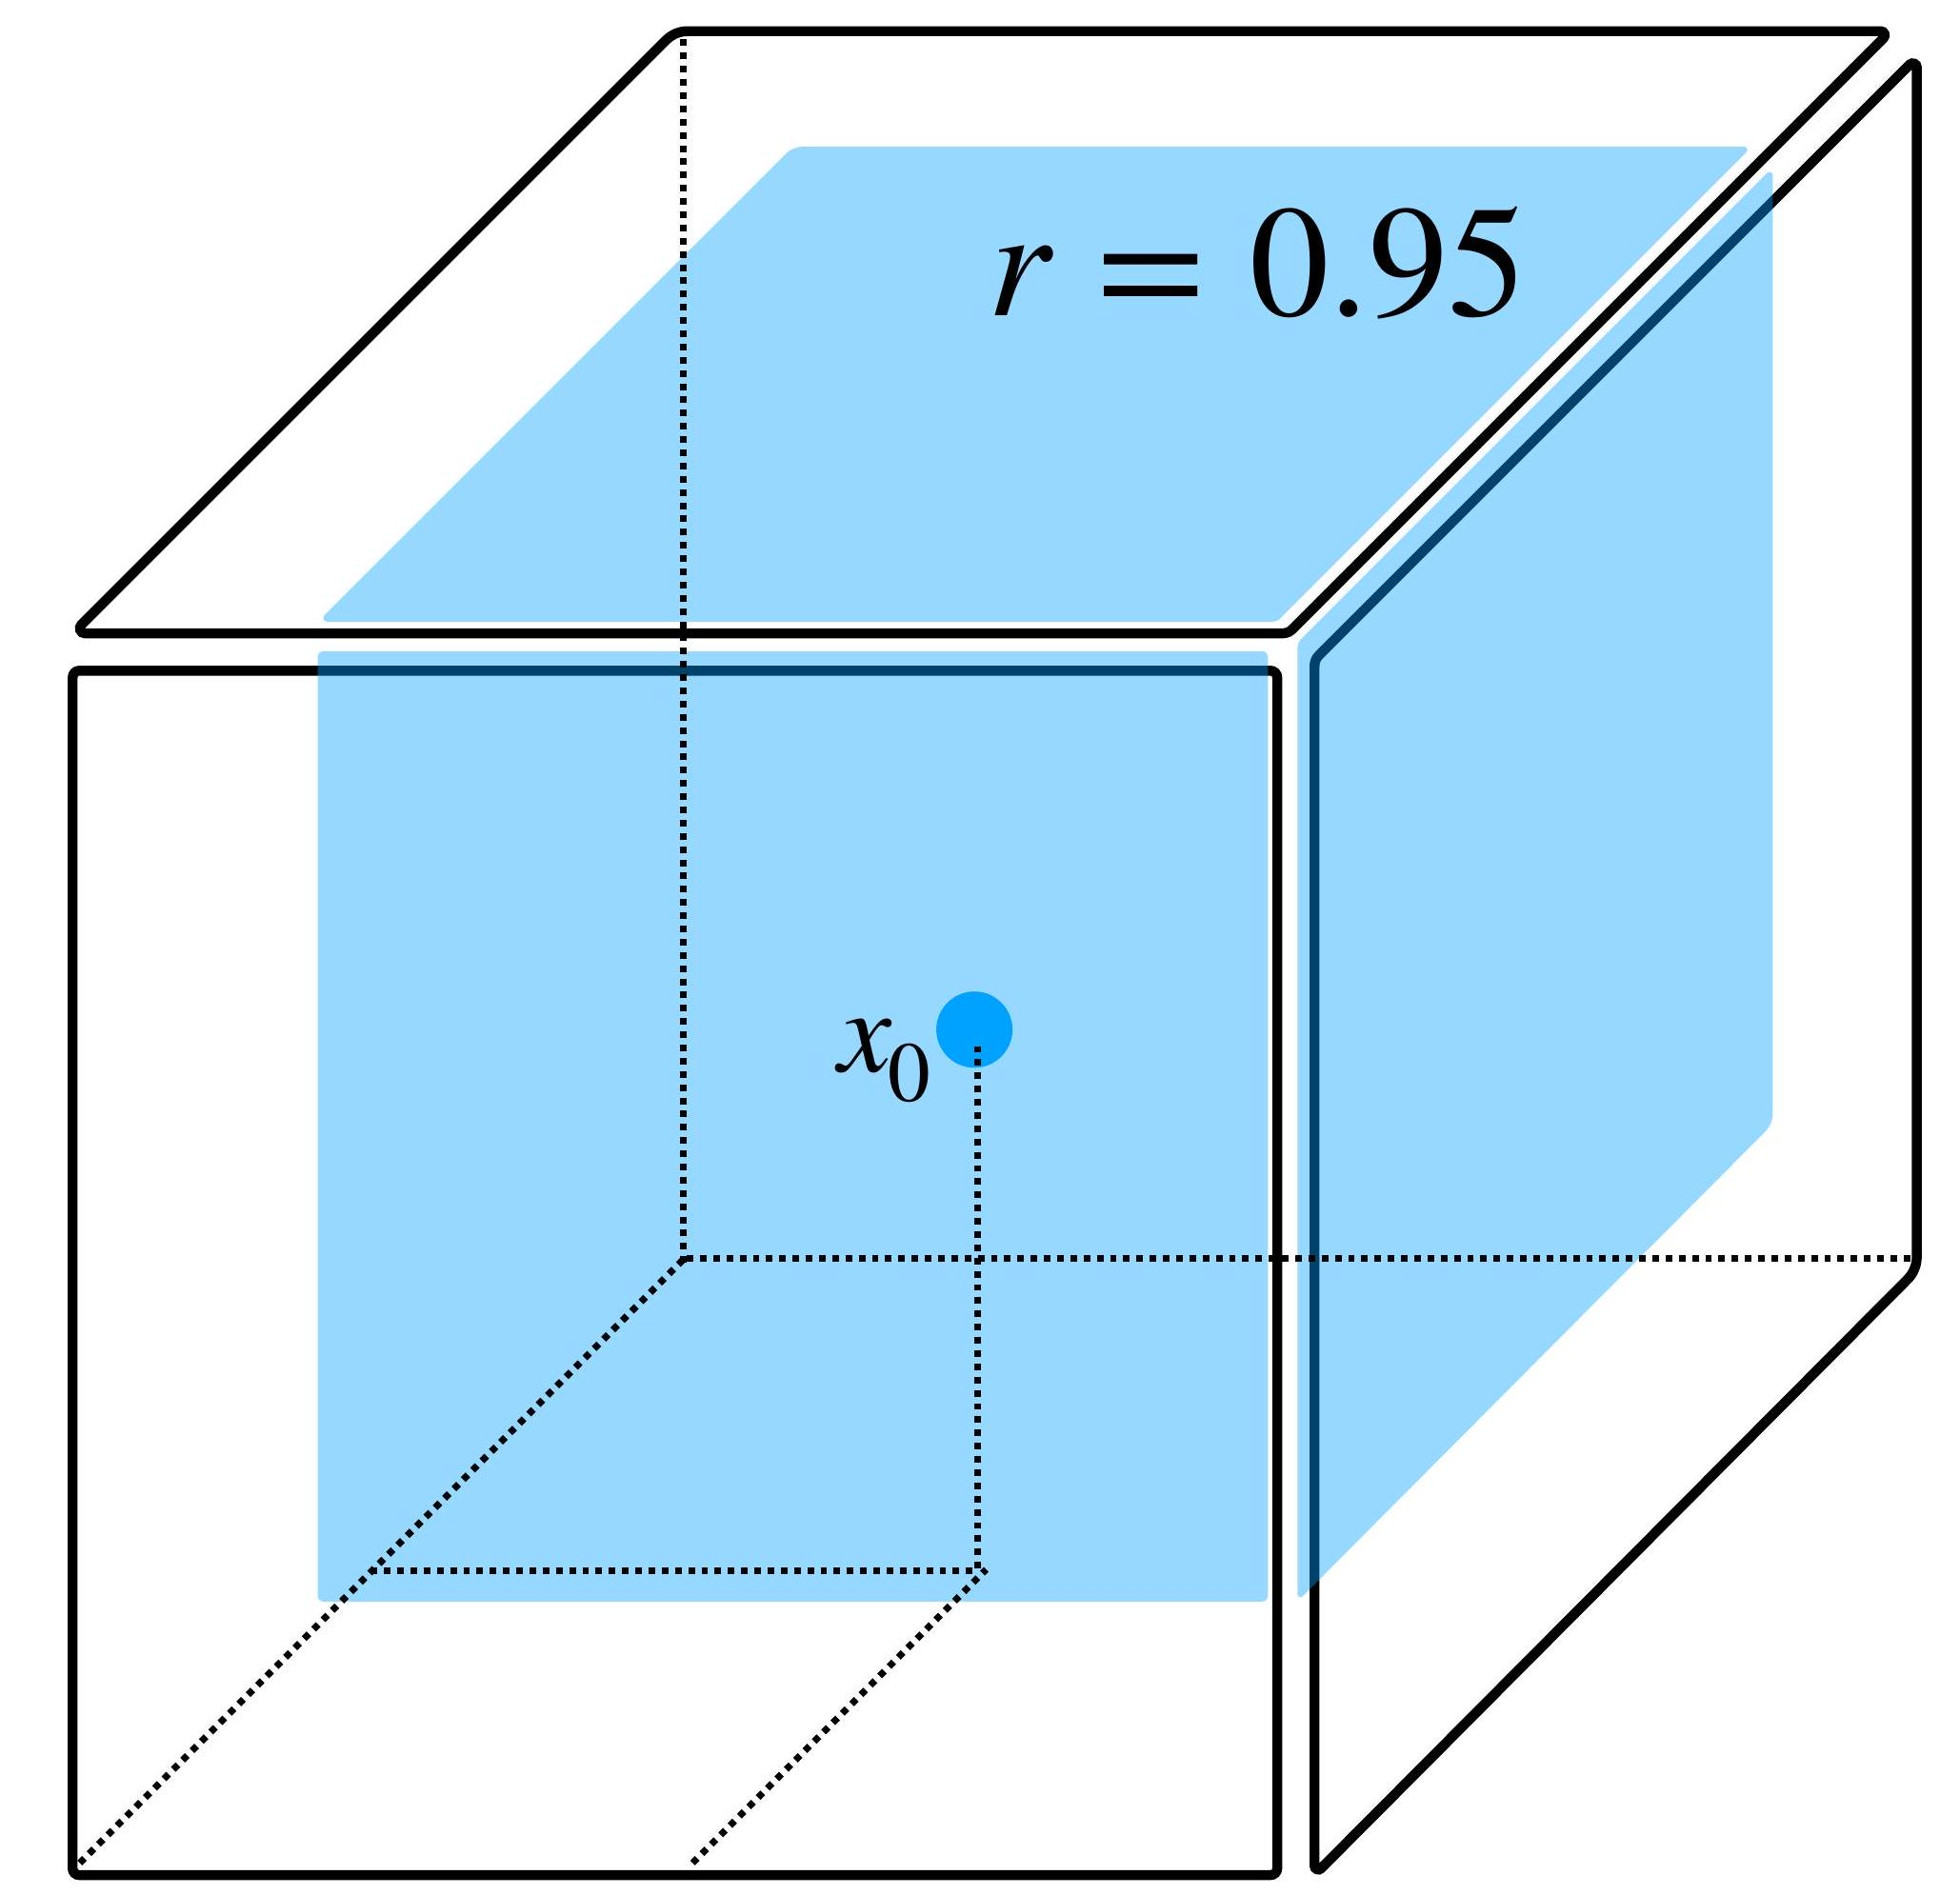
\includegraphics[max width=\textwidth]{2023_12_30_f937b0007b5d87b39f79g-26}
\end{center}

$X=[0,1]^{d}$

\section*{Curse of dimensionality}
Claim 2: In high-dimension, data-points are far from each other.

Consider $N$ i.i.d. points uniform in the $[0,1]^{d}$

$$
\mathbb{P}\left(\exists x_{i} \in \square\right) \geq 1 / 2 \Longrightarrow r \geq\left(1-\frac{1}{2^{1 / N}}\right)^{1 / d}
$$

Proof: $\mathbb{P}(x \notin \square)=1-r^{d}$

$$
\begin{aligned}
& \mathbb{P}\left(x_{i} \notin \quad, \forall i \leq N\right)=\left(1-r^{d}\right)^{N} \\
& \mathbb{P}\left(\exists x_{i} \in \square\right)=1-\left(1-r^{d}\right)^{N}
\end{aligned}
$$

For $d=10, N=500$, we have $r \geq 0.52$

\begin{center}
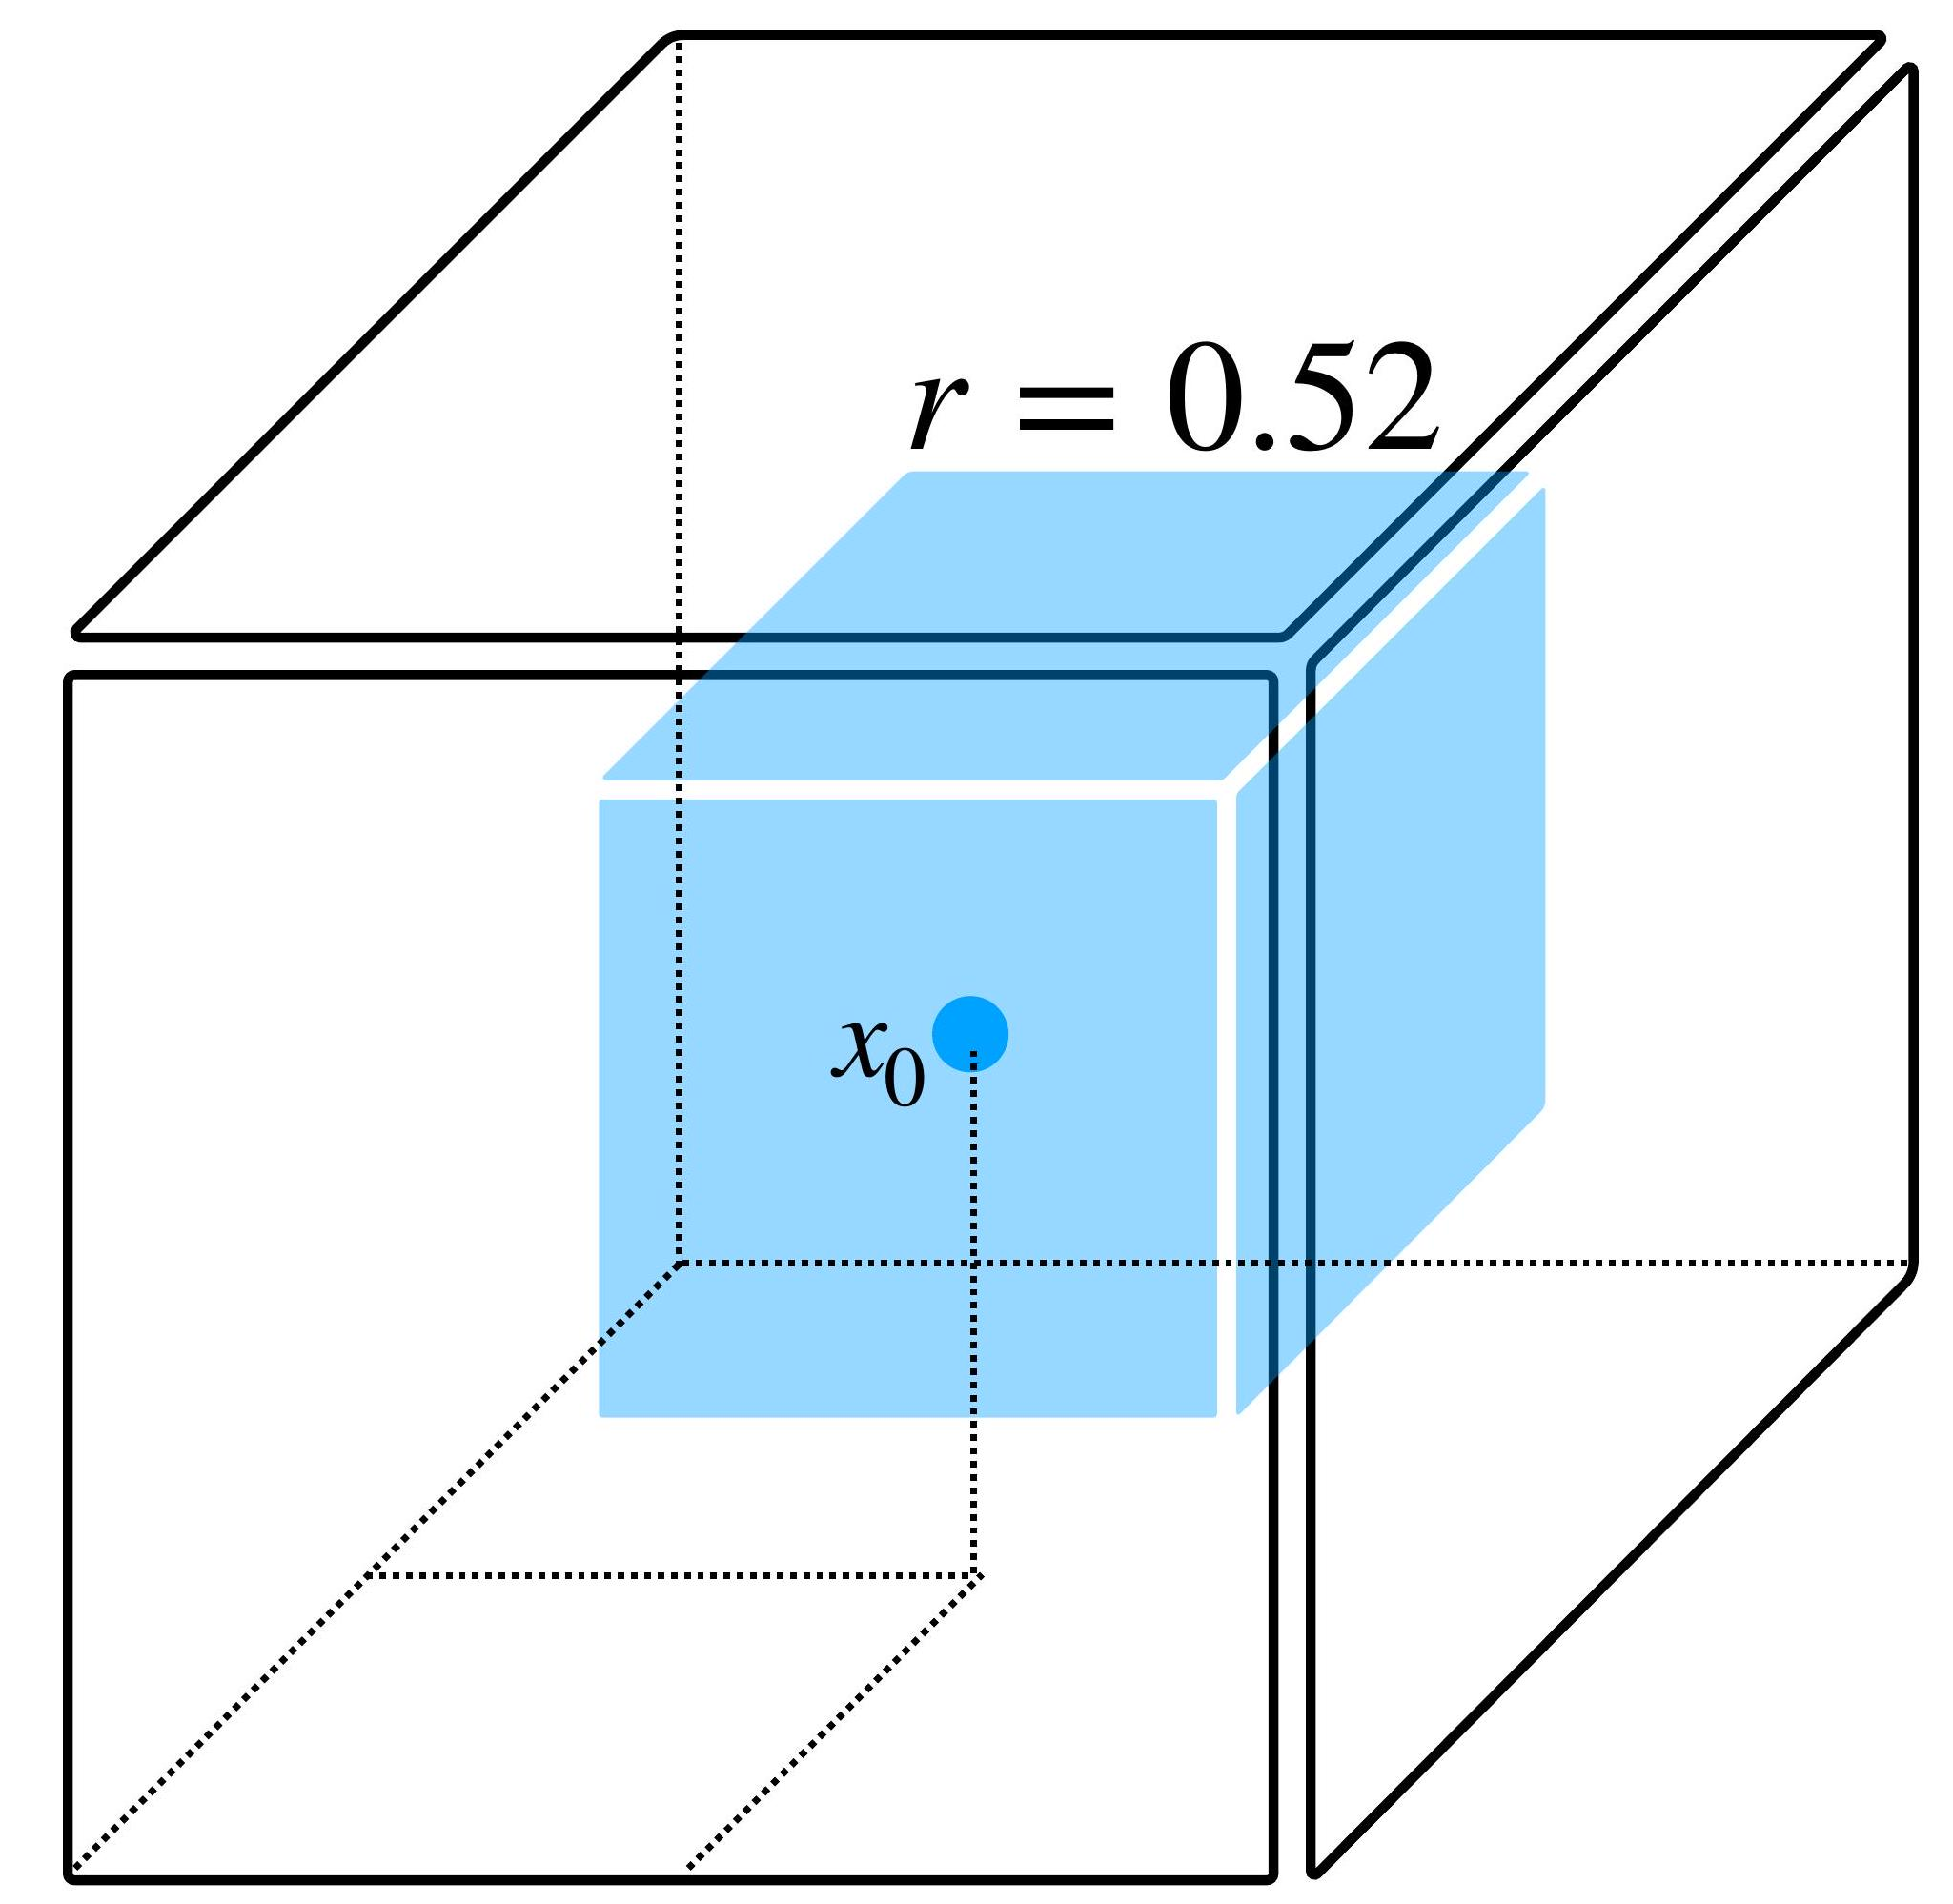
\includegraphics[max width=\textwidth]{2023_12_30_f937b0007b5d87b39f79g-27}
\end{center}

$$
\mathscr{X}=[0,1]^{d}
$$

\section*{Generalization bound for 1-NN}
Setup: $(X, Y) \sim \mathscr{D}$ over $\mathscr{X} \times \mathscr{Y}=[0,1]^{d} \times\{0,1\}$

Goal: Bound the classification error:

$$
L(f)=\mathbb{P}_{(X, Y) \sim D}(Y \neq f(X))
$$

Baseline:

\begin{itemize}
  \item Bayes classifier: minimizes $L$ over all classifiers
\end{itemize}

$$
f_{*}(x)=1_{\eta(x) \geq 1 / 2} \text { where } \eta(x)=\mathbb{P}(Y=1 \mid X=x)
$$

\begin{itemize}
  \item Bayes risk: represents the minimum probability of misclassification
\end{itemize}

$$
L\left(f_{*}\right)=\mathbb{P}\left(f_{*}(X) \neq Y\right)=\mathbb{E}_{X \sim D_{X}}[\min \{\eta(X), 1-\eta(X)\}]
$$

\section*{Generalization bound for 1-NN}
\begin{center}
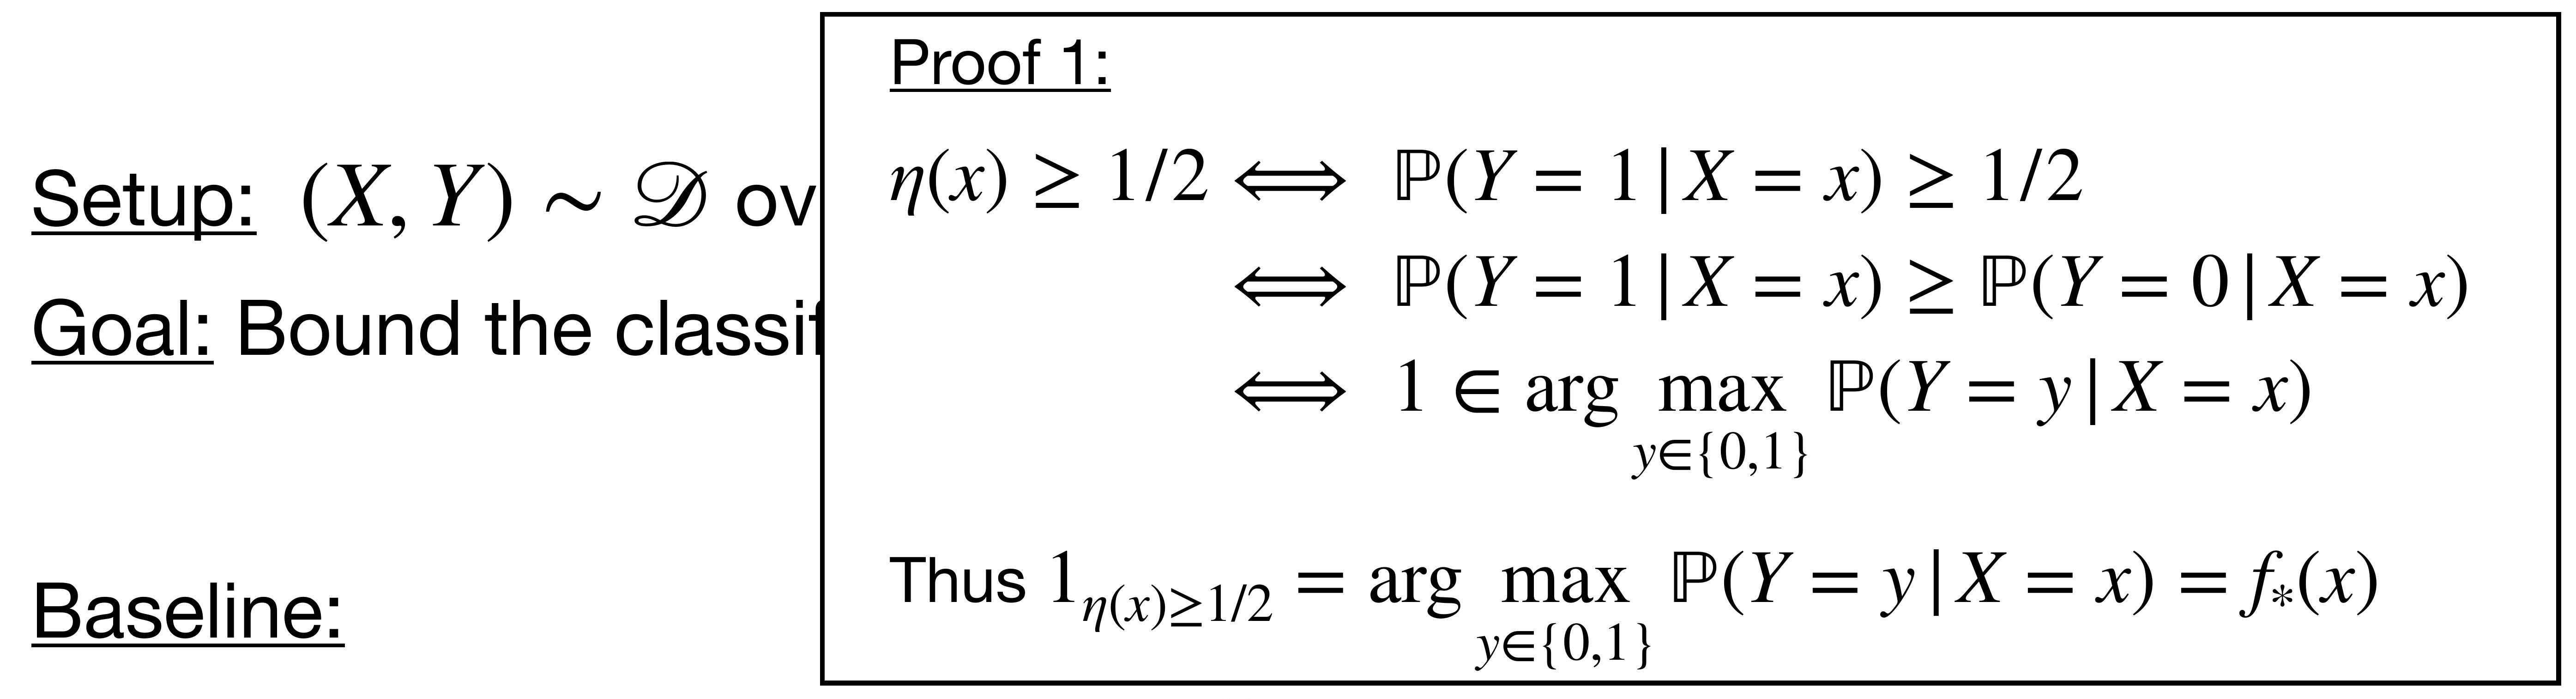
\includegraphics[max width=\textwidth]{2023_12_30_f937b0007b5d87b39f79g-29}
\end{center}

\begin{itemize}
  \item Bayes classifier: minimizes $L$ over all classifiers
\end{itemize}

$$
f_{*}(x)=1_{\eta(x) \geq 1 / 2} \text { where } \eta(x)=\mathbb{P}(Y=1 \mid X=x)
$$

\begin{itemize}
  \item Bayes risk: represents the minimum probability of misclassification
\end{itemize}

$$
L\left(f_{*}\right)=\mathbb{P}\left(f_{*}(X) \neq Y\right)=\mathbb{E}_{X \sim \mathscr{D}_{X}}[\min \{\eta(X), 1-\eta(X)\}]
$$

\section*{Generalization bound for 1-NN}
Proof 2:

$$
\begin{aligned}
& L\left(f_{*}\right)=\mathbb{E}_{(X, Y) \sim \mathscr{D}}\left[1_{f_{*}(X) \neq Y}\right]
\end{aligned}
$$

\begin{center}
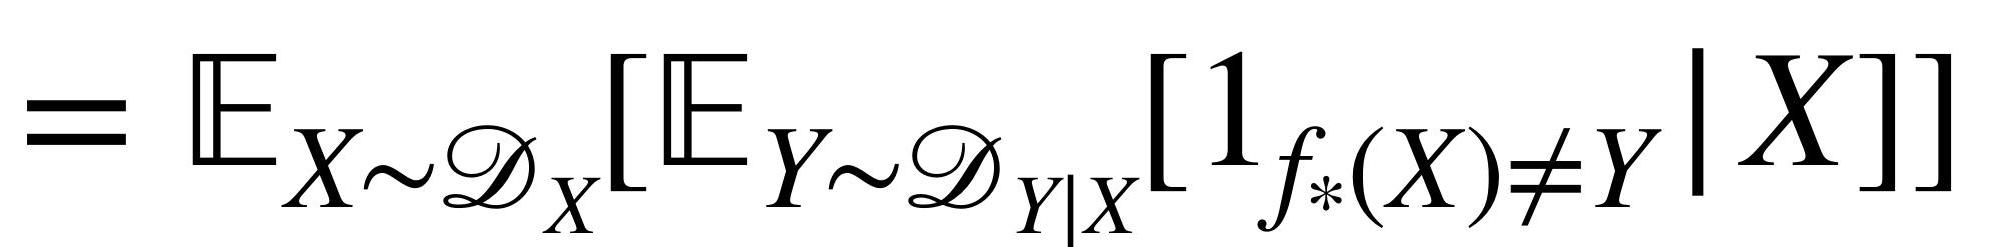
\includegraphics[max width=\textwidth]{2023_12_30_f937b0007b5d87b39f79g-30}
\end{center}

$$
\begin{aligned}
& =\mathbb{E}_{X \sim \mathscr{D}_{X}}\left[\mathbb{E}_{Y \sim \mathscr{D}_{Y \mid X}}\left[1_{f_{*}(X) \neq Y} \mid X\right] 1_{\eta(X) \geq 1 / 2}+E_{Y \sim \mathscr{D}_{Y \mid X}}\left[1_{f_{*}(X) \neq Y} \mid X\right] 1_{\eta(X)<1 / 2}\right] \\
& =\mathbb{E}_{X \sim \mathscr{D}_{X}}\left[\mathbb{E}_{Y \sim \mathscr{D}_{Y \mid X}}\left[1_{1 \neq Y} \mid X\right] 1_{\eta(X) \geq 1 / 2}+E_{Y \sim \mathscr{D}_{Y \mid X}}\left[1_{0 \neq Y} \mid X\right] 1_{\eta(X)<1 / 2}\right] \\
& =\mathbb{E}_{X \sim D_{X}}\left[\mathbb{P}(Y=0 \mid X) 1_{\eta(X) \geq 1 / 2}+\mathbb{P}(Y=1 \mid X) 1_{\eta(X)<1 / 2}\right] \\
& =\mathbb{E}_{X \sim \mathscr{D}_{X}}[\min \{\eta(X), 1-\eta(X)\}]
\end{aligned}
$$

\begin{itemize}
  \item Bayes risk: represents the minimum probability of misclassification
\end{itemize}

$$
L\left(f_{*}\right)=\mathbb{P}\left(f_{*}(X) \neq Y\right)=\mathbb{E}_{X \sim D_{X}}[\min \{\eta(X), 1-\eta(X)\}]
$$

\section*{Generalization bound for 1-NN}
Assumption: $\exists c \geq 0, \forall x, x^{\prime} \in \mathscr{X}$ :

$$
\left|\eta(x)-\eta\left(x^{\prime}\right)\right| \leq c\left\|x-x^{\prime}\right\|_{2}
$$

$\Rightarrow$ Nearby points are likely to share the same label

Claim:

$$
\leq 2 L\left(f_{*}\right)+4 c \sqrt{d} N^{-\frac{1}{d+1}}
$$

\begin{center}

\includegraphics[max width=\textwidth]{2023_12_30_f937b0007b5d87b39f79g-31}
\end{center}

Interpretation:

For constant $d$ and $N \rightarrow \infty: \mathbb{E}_{S_{\text {train }}}\left[L\left(f_{S_{\text {train }}}\right)\right] \leq 2 L\left(f_{*}\right)$

geometric term: average distance between a random point and its closest neighbor

To achieve a constant error, we need $N \propto d^{(d+1) / 2}$ - curse of dimensionality

Despite common belief: Interpolation method can generalize well

\section*{Proof}
We want to bound

$$
\mathbb{E}_{S_{\text {train }}}\left[L\left(f_{S_{\text {train }}}\right)\right]=\mathbb{E}_{S_{\text {train }}}\left[\mathbb{P}_{(X, Y) \sim \mathscr{D}}\left[f_{S_{\text {train }}}(X) \neq Y\right]\right]
$$

We first sample $N$ unlabeled examples $S_{\text {train }, X}=\left(X_{1}, \cdots X_{N}\right) \sim \mathscr{D}_{X}$, an unlabeled example $X \sim \mathscr{D}_{X}$ and define $X^{\prime}=\operatorname{nbh}_{S_{\text {train }, 1}}(X)$

Finally we sample $Y \sim \eta(X)$ and $Y^{\prime} \sim \eta\left(X^{\prime}\right)$

We have:

$$
\begin{aligned}
& \mathbb{E}_{S_{\text {train }}}\left[L\left(f_{S_{\text {train }}}\right)\right]=\mathbb{E}_{S_{\text {train }, X}, X \sim D_{X}, Y \sim \eta(X), Y^{\prime} \sim \eta\left(X^{\prime}\right)}\left[1_{Y \neq f_{S_{\text {train }}(X)}}\right] \\
& =\mathbb{E}_{S_{\text {train, } X}, X \sim \mathscr{D}_{X}, Y \sim \eta(X), Y^{\prime} \sim \eta\left(X^{\prime}\right)}\left[1_{Y \neq Y^{\prime}}\right] \\
& =\mathbb{E}_{S_{\text {train }, X}, X \sim \mathscr{D}_{X}}\left[\mathbb{P}_{Y \sim \eta(X), Y^{\prime} \sim \eta\left(X^{\prime}\right)}\left(Y \neq Y^{\prime}\right)\right]
\end{aligned}
$$

\section*{Proof}
Consider two points $x, x^{\prime} \in[0,1]^{d}$.

Sample their labels $Y \sim \eta(x)$ and $Y^{\prime} \sim \eta\left(x^{\prime}\right)$

Claim:

$$
\mathbb{P}\left(Y^{\prime} \neq Y\right) \leq 2 \min \{\eta(x), 1-\eta(x)\}+c\left\|x-x^{\prime}\right\|
$$

\begin{itemize}
  \item Simple case: $x=x^{\prime}$
\end{itemize}

$$
\begin{aligned}
\mathbb{P}\left(Y^{\prime} \neq Y\right) & =\mathbb{E}\left[1_{Y^{\prime} \neq Y} 1_{Y^{\prime}=1}+1_{Y^{\prime} \neq Y^{\prime}} 1_{Y^{\prime}=0}\right] \\
& =\mathbb{P}\left(Y^{\prime}=1\right) \mathbb{P}(Y=0)+\mathbb{P}\left(Y^{\prime}=1\right) \mathbb{P}(Y=0) \\
& =2 \eta(x)(1-\eta(x)) \\
& \leq 2 \min \{\eta(x), 1-\eta(x)\}
\end{aligned}
$$

Case 1:

$\mathbf{Y}=\mathbf{0}(1-\eta(x))$

$Y^{\prime}=1 \quad \eta(x)$

Case 2:

$\mathrm{Y}=\mathbf{1} \quad \eta(x)$

$Y^{\prime}=0 \quad(1-\eta(x))$

\section*{Proof}
\begin{itemize}
  \item General case:
\end{itemize}

$$
\begin{aligned}
\mathbb{P}\left(Y \neq Y^{\prime}\right)= & \eta(x)\left(1-\eta\left(x^{\prime}\right)\right)+\eta\left(x^{\prime}\right)(1-\eta(x)) \\
= & \eta(x)(1-\eta(x))+\eta(x)\left(\eta(x)-\eta\left(x^{\prime}\right)\right) \\
& \quad+\eta(x)(1-\eta(x))+\left(\eta\left(x^{\prime}\right)-\eta(x)\right)(1-\eta(x)) \\
= & 2 \eta(x)(1-\eta(x))+(2 \eta(x)-1)\left(\eta(x)-\eta\left(x^{\prime}\right)\right) \\
& \leq 2 \eta(x)(1-\eta(x))+|(2 \eta(x)-1)|\left|\eta(x)-\eta\left(x^{\prime}\right)\right| \\
& \leq 2 \eta(x)(1-\eta(x))+\left|\eta(x)-\eta\left(x^{\prime}\right)\right| \\
& \leq 2 \eta(x)(1-\eta(x))+c\left\|x-x^{\prime}\right\| \\
& \leq 2 \min \{\eta(x), 1-\eta(x)\}+c\left\|x-x^{\prime}\right\|
\end{aligned}
$$

\section*{Proof}
$$
\begin{aligned}
\mathbb{E}_{S_{\text {train }}}\left[L \left(f_{\left.\left.S_{\text {train }}\right)\right]}\right.\right. & =\mathbb{E}_{S_{\text {train, }, X}, X \sim \mathscr{D}_{X}, Y \sim \eta(X), Y^{\prime} \sim \eta\left(X^{\prime}\right)}\left[1_{Y \neq f_{\text {train }(X)}}\right] \\
& =\mathbb{E}_{S_{\text {train, }, X}, X \sim \mathscr{D}_{X}, Y \sim \eta(X), Y^{\prime} \sim \eta\left(X^{\prime}\right)}\left[1_{Y \neq Y^{\prime}}\right] \\
& =\mathbb{E}_{S_{\text {train }, X}, X \sim D_{X}}\left[\mathbb{P}_{Y \sim \eta(X), Y^{\prime} \sim \eta(X)}\left(Y \neq Y^{\prime}\right)\right] \\
& \leq \mathbb{E}_{S_{\text {train }, X}, X \sim \mathscr{D}_{X}}\left[2 \min \{\eta(X), 1-\eta(X)\}+c\left\|X-X^{\prime}\right\|\right] \\
& \leq 2 L\left(f_{*}\right)+c \mathbb{E}_{S_{\text {train }}, X \sim \mathscr{D}_{X}}\left[\left\|X-\operatorname{nbh}_{S_{\text {train }}, 1}(X)\right\|\right]
\end{aligned}
$$

\section*{Bound on the geometric term}
Consider a fresh sample $X \sim \mathscr{D}$ and denote by $p_{k}=\mathbb{P}\left(X \in\right.$ Box $\left._{k}\right)$

Consider the box which contains $X$. Two options:

\begin{itemize}
  \item The box contains an element of $S_{\text {train }}$ X has a neighbor in $S_{\text {train }}$ at distance at most $\sqrt{d} \varepsilon$
\end{itemize}

It happens with probability $1-\left(1-p_{k}\right)^{N}$

Proof: Consider the worst case:

$$
\left\|X-x_{i}\right\|=\sqrt{\sum_{i=1}^{d} \varepsilon^{2}}=\sqrt{d} \varepsilon
$$

\begin{center}
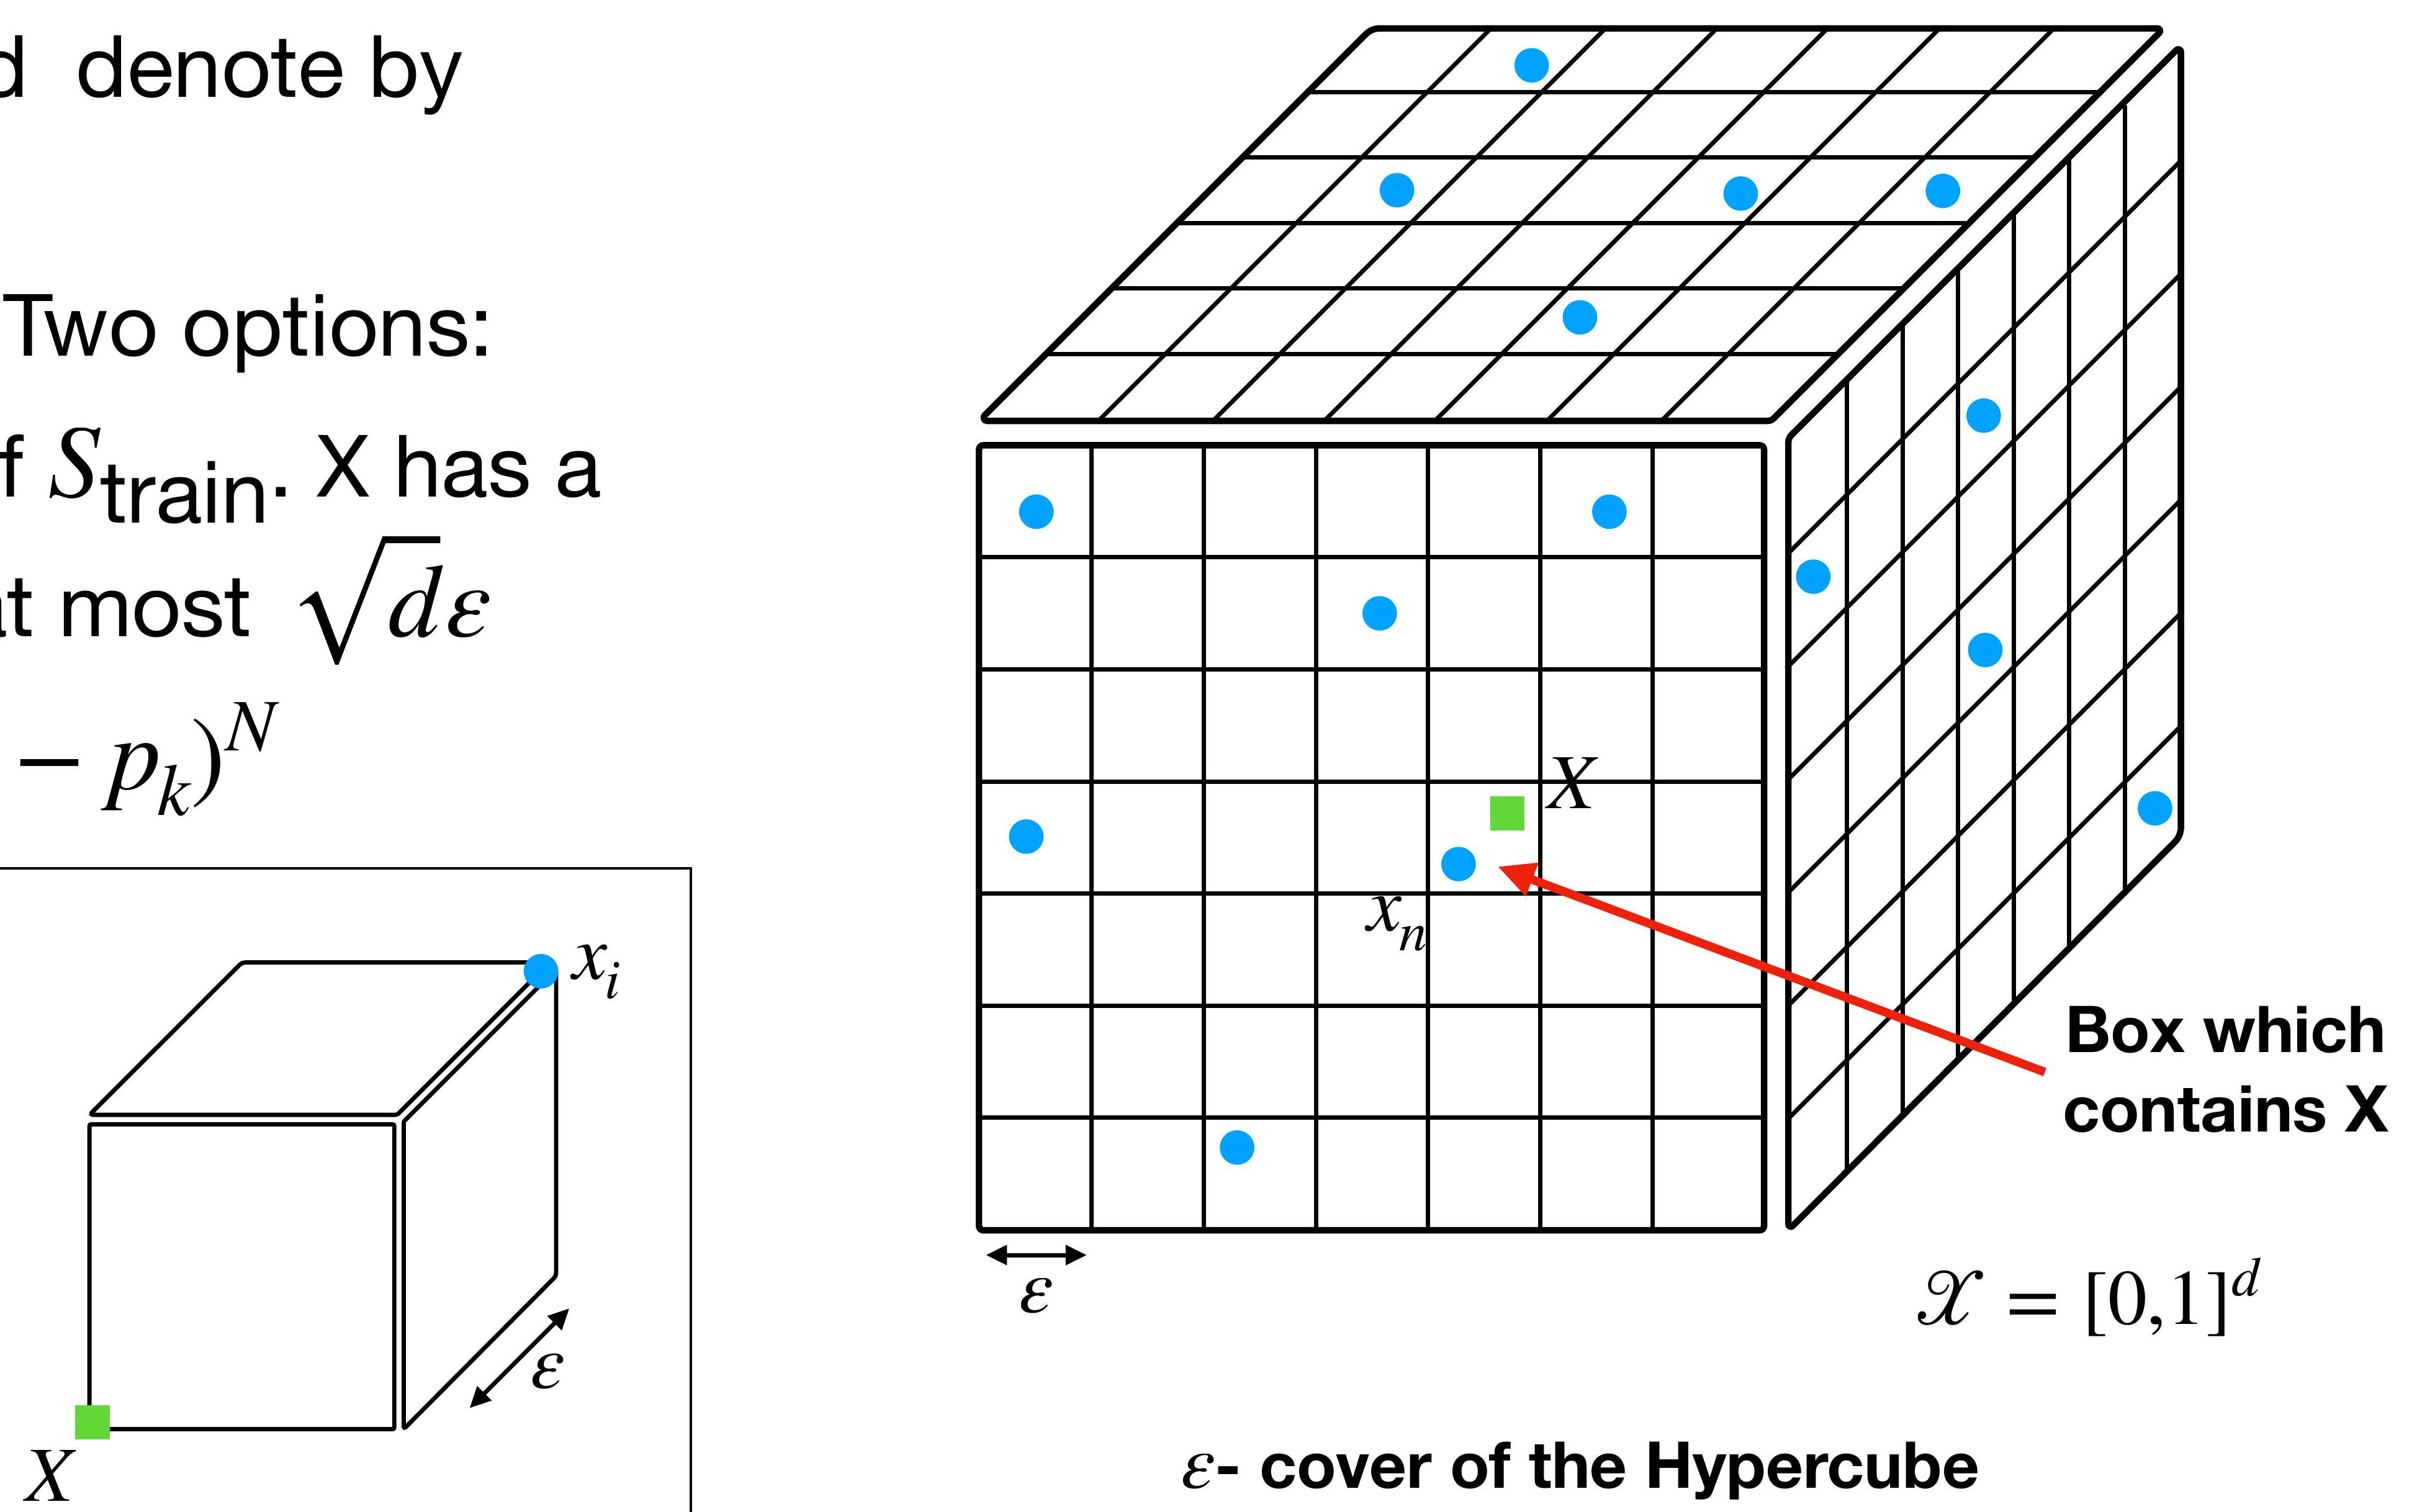
\includegraphics[max width=\textwidth]{2023_12_30_f937b0007b5d87b39f79g-36}
\end{center}

\section*{Bound on the geometric term}
Consider a fresh sample $X \sim \mathscr{D}$ and denote by $p_{k}=\mathbb{P}\left(X \in\right.$ Box $\left._{k}\right)$

Consider the box which contains $X$. Two options:

\begin{itemize}
  \item The box contains an element of $S_{\text {train }} \mathrm{X}$ has a neighbor in $S_{\text {train }}$ at distance at most $\sqrt{d} \varepsilon$
\end{itemize}

It happens with probability $1-\left(1-p_{k}\right)^{N}$

\begin{itemize}
  \item There is no element of $S_{\text {train }}$. The nearest neighbor of $\mathrm{X}$ can be at worst at a distance $\sqrt{d}$ It happens with probability $\left(1-p_{k}\right)^{N}$
\end{itemize}

\begin{center}
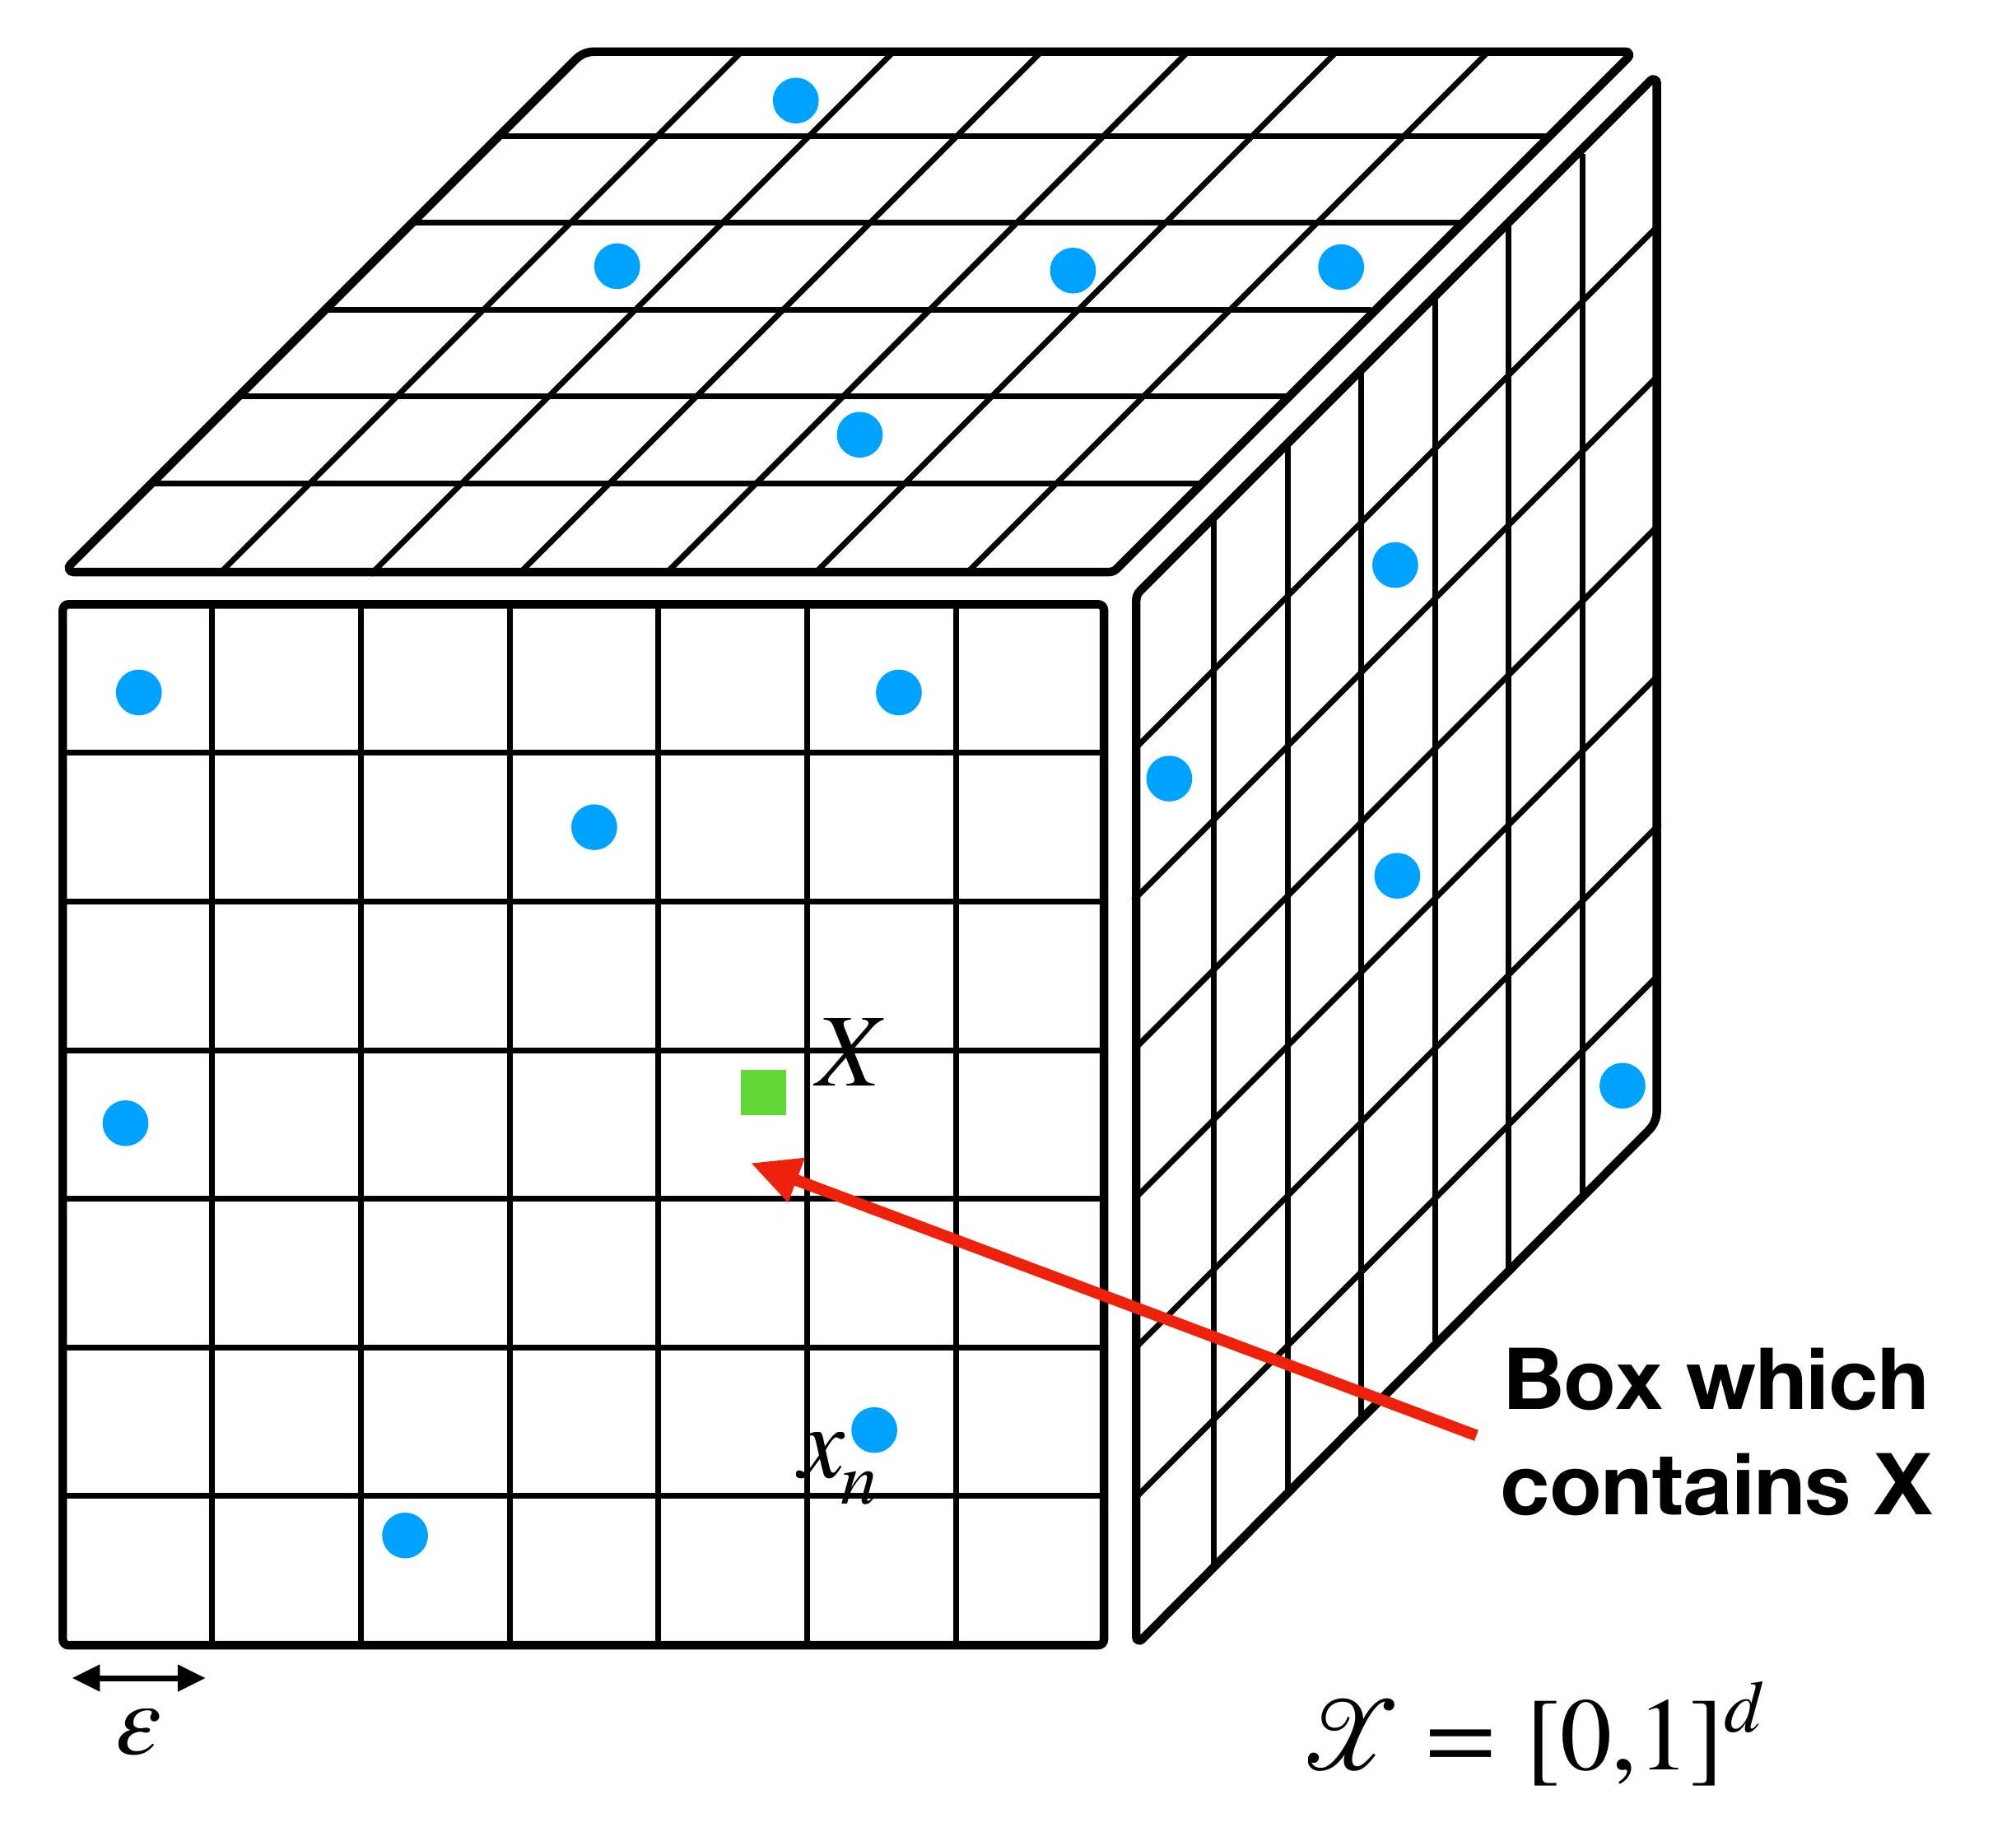
\includegraphics[max width=\textwidth]{2023_12_30_f937b0007b5d87b39f79g-37}
\end{center}

\section*{Bound on the geometric term}
Consider a fresh sample $X \sim \mathscr{D}$ and denote by

$$
p_{k}=\mathbb{P}\left(X \in \mathrm{Box}_{k}\right)
$$

\begin{center}
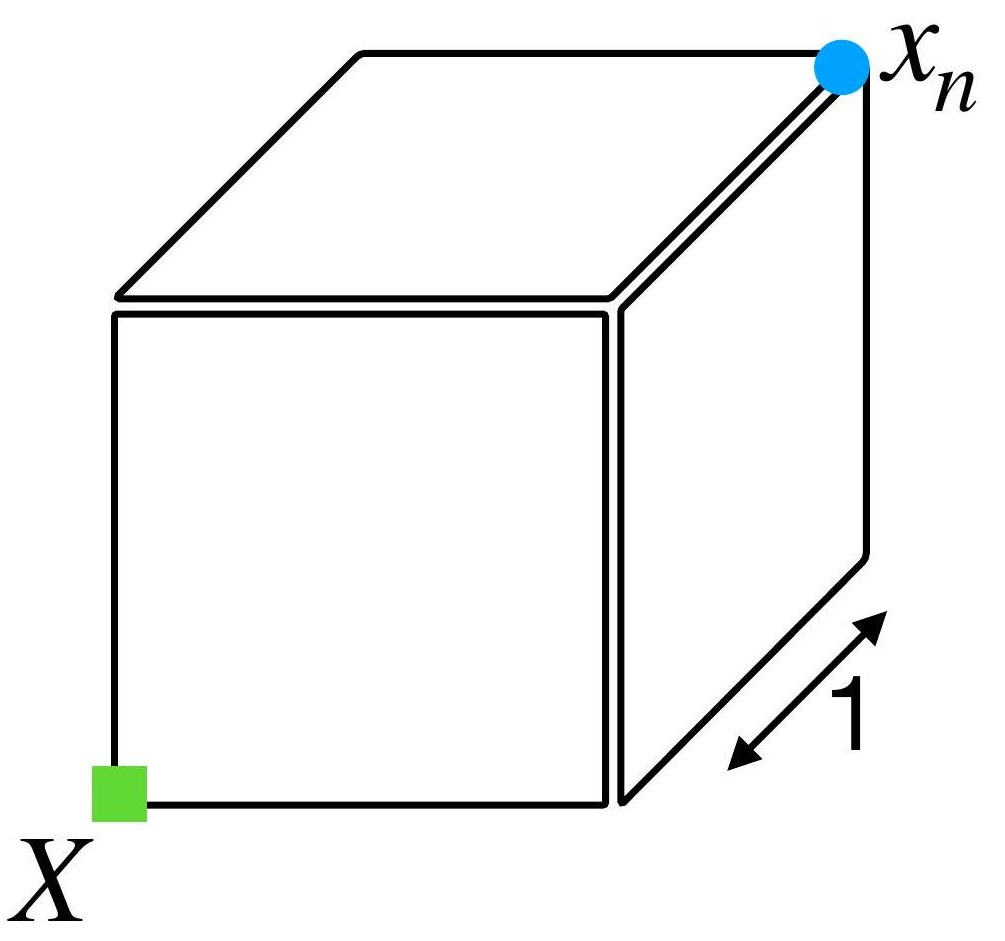
\includegraphics[max width=\textwidth]{2023_12_30_f937b0007b5d87b39f79g-38}
\end{center}

\section*{Bound on the geometric term}
$\mathbb{E}[\|X-\mathrm{nbh}(X)\|] \leq \sum_{k} p_{k}\left[\left(1-p_{k}\right)^{N} \sqrt{d}+\left(1-\left(1-p_{k}\right)^{N}\right) \sqrt{d} \varepsilon\right]$

Claim: The bound is derived by optimizing over $p_{k}$ and $\varepsilon$

Intuition:

\begin{itemize}
  \item If $p_{k}$ is large: it is likely that we pick that box but it is also likely that we find a training point in that box
  \item If $p_{k}$ is small, we are generally safe, as by its definition, this scenario occurs infrequently
\end{itemize}

\begin{center}
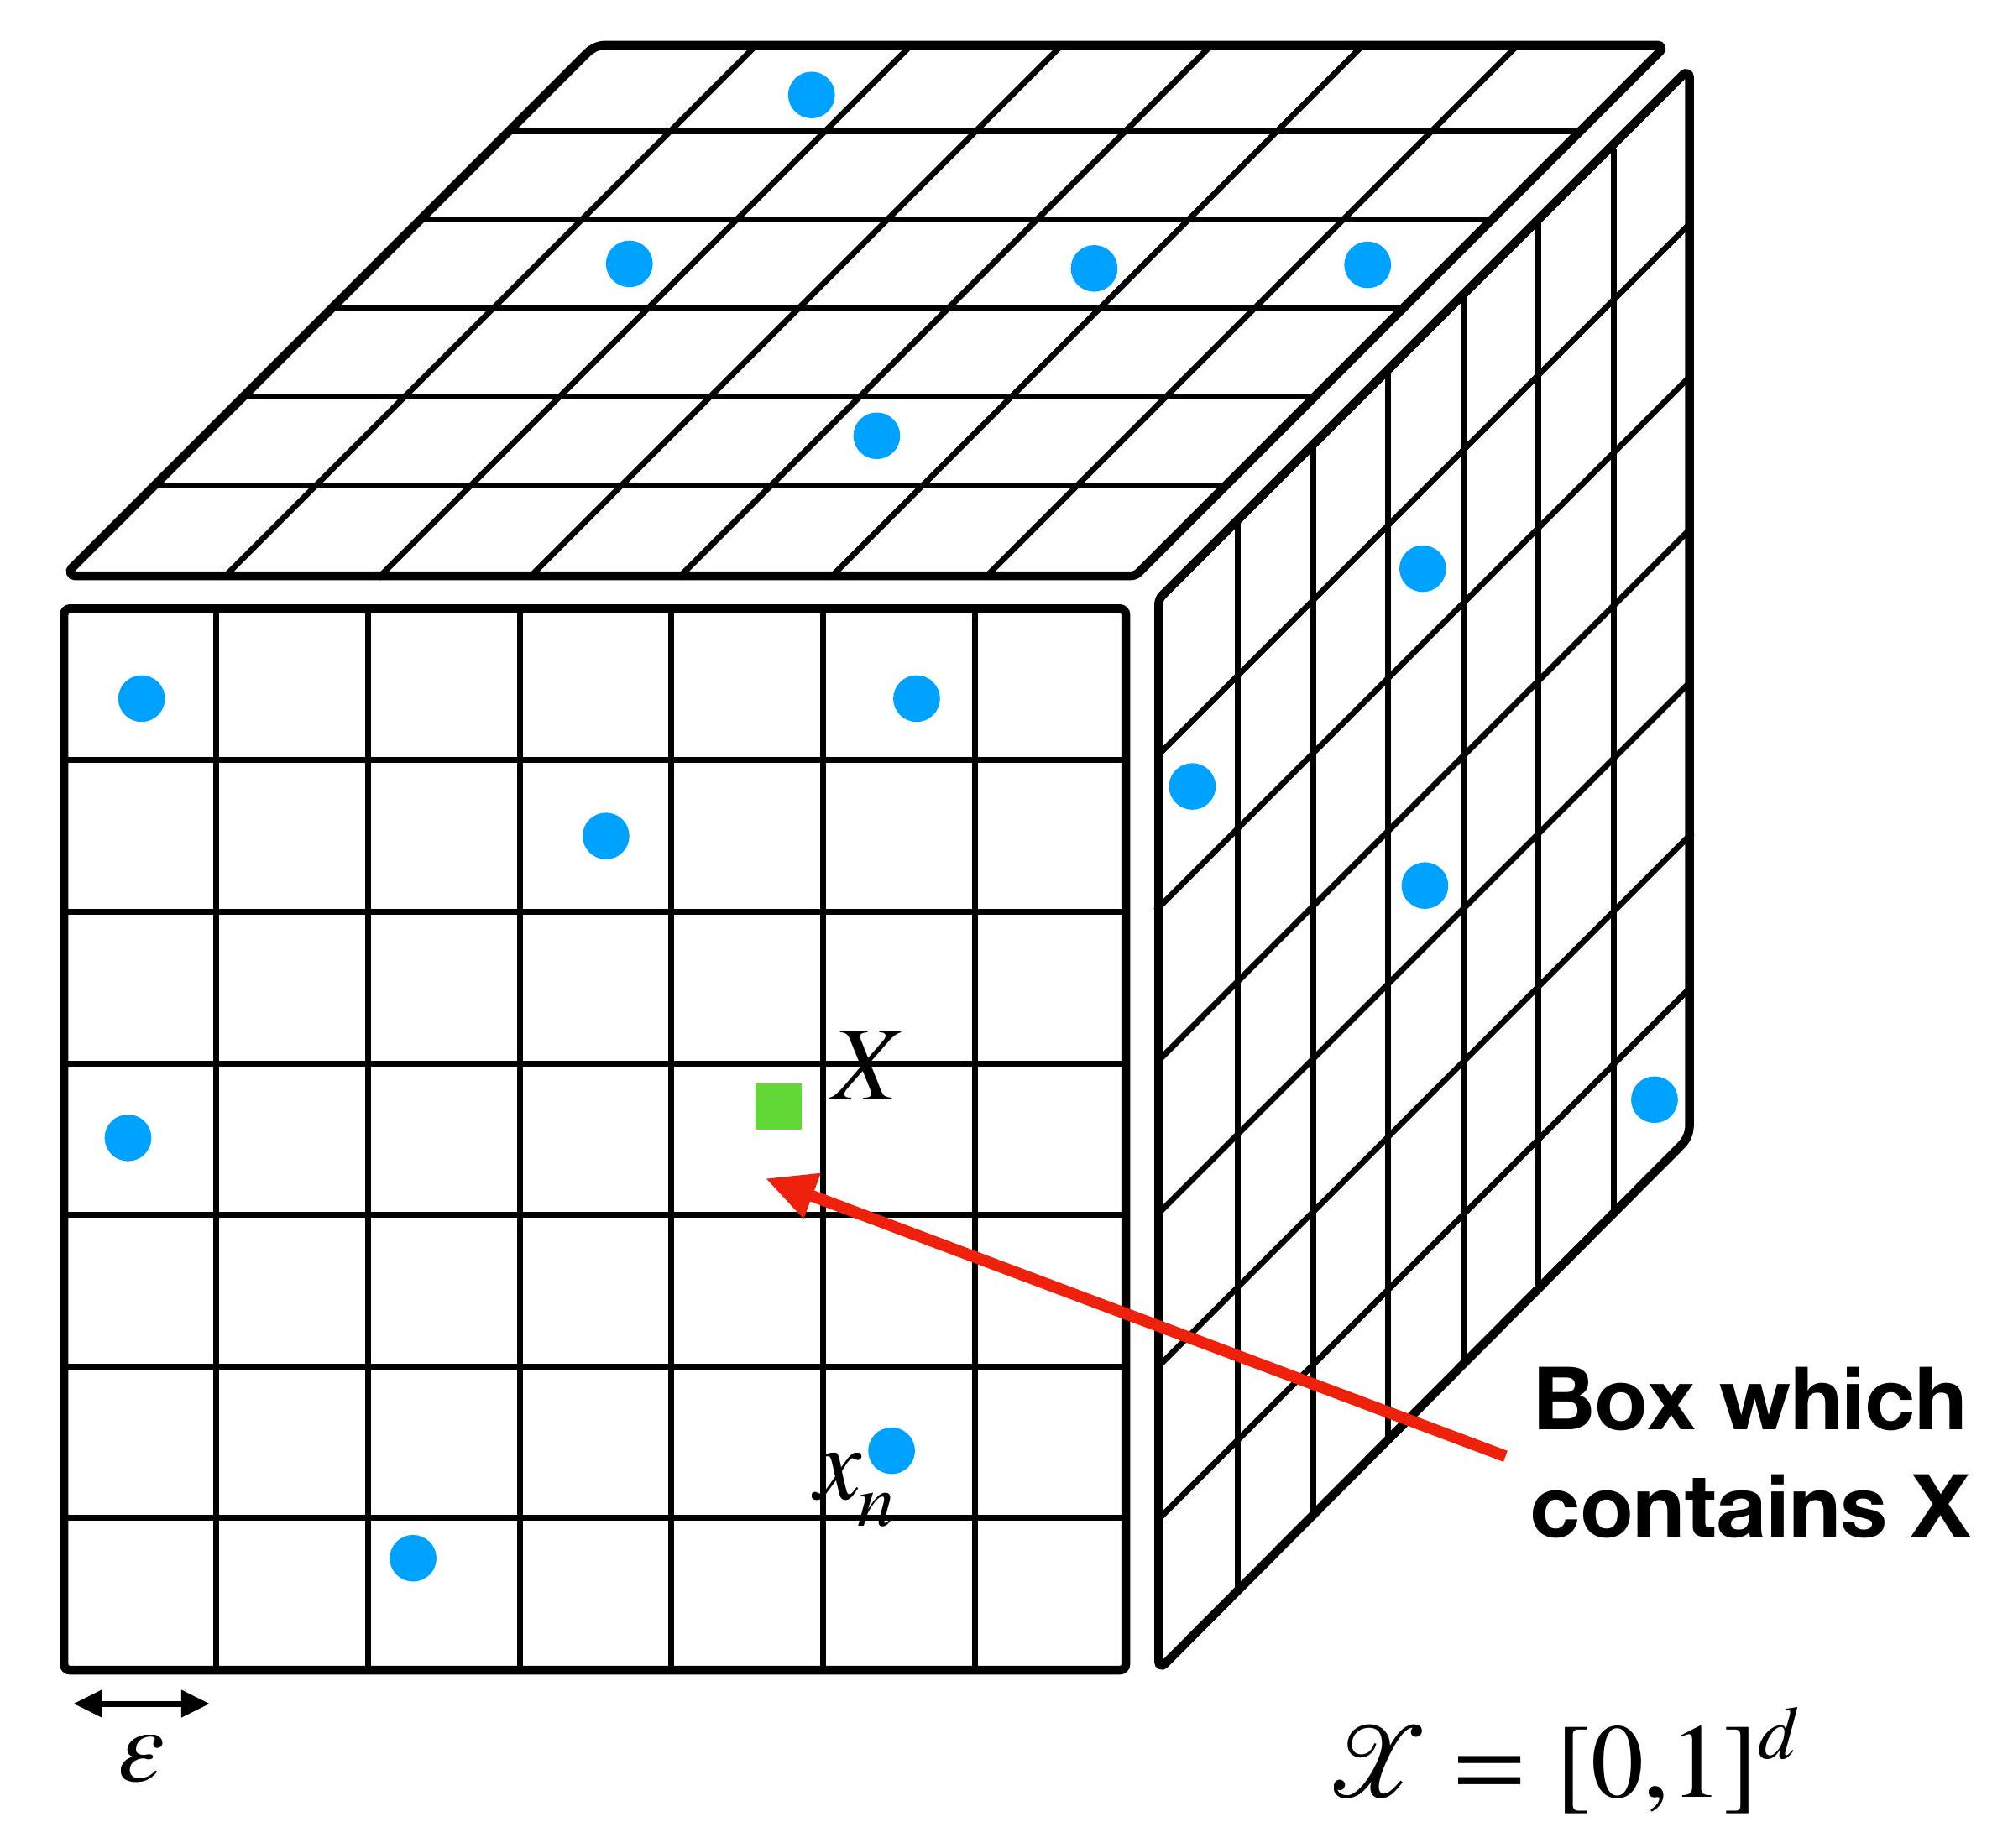
\includegraphics[max width=\textwidth]{2023_12_30_f937b0007b5d87b39f79g-39}
\end{center}

\section*{Nearest Neighbors is a local averaging method}
Local averaging methods aim to approximate the Bayes predictor directly - without the need for optimization

This is achieved by approximating the conditional distribution $p(y \mid x)$ by some $\hat{p}(y \mid x)$ These "plug-in" estimators are:

. $f(x) \in \arg \max \hat{\mathbb{P}}(Y=y \mid x)$ for classification with the $0-1$ loss $y \in \mathcal{Y}$

\begin{itemize}
  \item $f(x)=\hat{\mathbb{E}}[Y \mid x]=\int_{\mathscr{y}} y \hat{p}(y \mid x) d y$ for regression with the square loss
\end{itemize}

In the case of nearest neighbors:

$$
\hat{p}(y \mid x)=\sum_{n=1}^{N} \hat{w}_{n}(x) 1_{y=y_{n}}
$$

where $\hat{w}(x)=1 / k$ for the $k$ nearest neighbors ( 0 otherwise)

\section*{Recap}
\begin{itemize}
  \item k-NN: a local averaging method for regression and classification
  \item use a notion of distance to define neighborhoods ( $k$ nearest neighbors)
  \item the prediction is a function of these neighborhoods
\end{itemize}

e.g., majority selection for classification, weighted sum for regression

\begin{itemize}
  \item Bias-variance: small/large $k$ leads to low/high bias and high/low variance

  \item Curse of dimensionality: as $d \nearrow \infty$, it is harder to define local neighborhoods

  \item For $N \rightarrow \infty, 1-\mathrm{NN}$ is competitive with Bayes classifier

  \item $N$ needs to scale exponentially in $d$ to achieve the same error

\end{itemize}

\end{document}